\documentclass[a4paper,13pt,3p,twoside]{report}

\usepackage{scrextend}
\changefontsizes{13pt}
\usepackage[utf8]{vietnam}
\usepackage[top=2cm, bottom=2cm, left=3.5cm, right=2.5cm]{geometry}
\usepackage{xurl}
\usepackage{appendix}
\usepackage{babel}
\usepackage[table]{xcolor}
\usepackage{outlines}
\usepackage{graphicx}
\usepackage{fancybox}
\usepackage{indentfirst}
\usepackage{amsthm}
\usepackage{latexsym}
\usepackage{amsmath, amssymb, amsfonts, amsbsy}
\usepackage{times}
\usepackage{array}
\usepackage{enumitem}
\usepackage{titlesec}
\usepackage{titletoc}
\usepackage{chngcntr}
\usepackage{pdflscape}
\usepackage{afterpage}
\usepackage[ruled,vlined]{algorithm2e}
\usepackage{capt-of}
\usepackage{booktabs}
\usepackage{multirow}
\usepackage{fancyhdr}
\usepackage[font=small,labelfont=bf]{caption}
\renewcommand{\figurename}{Hình}
\renewcommand{\tablename}{Bảng}
\usepackage{listings}
\usepackage{float}
\usepackage{subcaption}
\usepackage[nonumberlist, nopostdot, nogroupskip, acronym]{glossaries}
\usepackage{glossary-superragged}
\setglossarystyle{longheaderborder}
\usepackage{setspace}
\usepackage{parskip}
\usepackage{tocbasic}

\renewcommand{\bibname}{TÀI LIỆU THAM KHẢO}
\usepackage[backend=biber,style=ieee]{biblatex}
\addbibresource{references.bib}

\makenoidxglossaries
\newglossaryentry{aerca}{type=\acronymtype, name={AERCA}, description={Auto-Encoder for Root Causal Analysis}, first={Auto-Encoder for Root Causal Analysis (AERCA)}}
\newglossaryentry{llm}{type=\acronymtype, name={LLM}, description={Large Language Model}, first={Large Language Model (LLM)}}
\newglossaryentry{bic}{type=\acronymtype, name={BIC}, description={Bayesian Information Criterion}, first={Bayesian Information Criterion (BIC)}}
\newglossaryentry{mse}{type=\acronymtype, name={MSE}, description={Mean Squared Error}, first={Mean Squared Error (MSE)}}
\newglossaryentry{dag}{type=\acronymtype, name={DAG}, description={Directed Acyclic Graph}, first={Directed Acyclic Graph (DAG)}}
\newglossaryentry{mhsa}{type=\acronymtype, name={MHSA}, description={Multi-Head Self-Attention}, first={Multi-Head Self-Attention (MHSA)}}
\newglossaryentry{yolo}{type=\acronymtype, name={YOLO}, description={You Only Look Once}, first={You Only Look Once (YOLO)}}
\newglossaryentry{iou}{type=\acronymtype, name={IoU}, description={Intersection over Union}, first={Intersection over Union (IoU)}}
\newglossaryentry{map}{type=\acronymtype, name={mAP}, description={mean Average Precision}, first={mean Average Precision (mAP)}}
\newglossaryentry{var}{type=\acronymtype, name={VAR}, description={Vector Autoregression}, first={Vector Autoregression (VAR)}}
\newglossaryentry{nms}{type=\acronymtype, name={NMS}, description={Non-Maximum Suppression}, first={Non-Maximum Suppression (NMS)}}
\newglossaryentry{json}{type=\acronymtype, name={JSON}, description={JavaScript Object Notation}, first={JavaScript Object Notation (JSON)}}

\fancypagestyle{plain}{%
\fancyhf{}
\fancyfoot[RO,RE]{\thepage}
\renewcommand{\headrulewidth}{0pt}
\renewcommand{\footrulewidth}{0pt}}

\setlength{\headheight}{18pt}

\def\TITLE{ĐỒ ÁN TỐT NGHIỆP}
\def\THESISTITLE{Suy luận tương quan với Mô hình Ngôn ngữ Lớn để Khám phá và Diễn giải hành vi học tập của học sinh trong lớp học}
\def\AUTHOR{Nguyễn Trung Long}
\def\STUDENTID{20224874}
\def\PROGRAM{Khoa học máy tính}
\def\DEPARTMENT{Khoa học máy tính}
\def\SUPERVISOR{PGS. TS. Phạm Văn Hải}
\def\SCHOOL{Công nghệ Thông tin và Truyền thông}
\def\LOCATIONDATE{HÀ NỘI, 06/2026}

\titleformat
    {\chapter}
    [hang]
    {\centering\bfseries}
    {CHƯƠNG \thechapter.\ }
    {0pt}
    {}
    []
\titlespacing*{\chapter}{0pt}{-20pt}{20pt}

\titleformat
    {\section}
    [hang]
    {\bfseries}
    {\thechapter.\arabic{section}\ \ \ \ }
    {0pt}
    {}
    []
\titlespacing{\section}{0pt}{\parskip}{0.5\parskip}

\titleformat
    {\subsection}
    [hang]
    {\bfseries}
    {\thechapter.\arabic{section}.\arabic{subsection}\ \ \ \ }
    {0pt}
    {}
    []
\titlespacing{\subsection}{30pt}{\parskip}{0.5\parskip}

\renewcommand\thesubsubsection{\alph{subsubsection}}
\titleformat
    {\subsubsection}
    [hang]
    {\bfseries}
    {\alph{subsubsection},\ }
    {0pt}
    {}
    []
\titlespacing{\subsubsection}{50pt}{\parskip}{0.5\parskip}

\usepackage{hyperref}
\hypersetup{pdfborder={0 0 0}}
\hypersetup{pdftitle={\THESISTITLE}, pdfauthor={\AUTHOR}}
\usepackage[all]{hypcap}

\graphicspath{{figures/}{doan/Hinh_ve/}}
\counterwithin{figure}{chapter}
\counterwithin{table}{chapter}
\numberwithin{equation}{chapter}

\title{\bf \TITLE}
\author{\AUTHOR}
\setcounter{secnumdepth}{3}

\theoremstyle{definition}
\newtheorem{example}{Ví dụ}[chapter]

\onehalfspacing
\setlength{\parskip}{6pt}
\setlength{\parindent}{15pt}

\newcommand{\makefrontcover}{%
\begin{titlepage}
\thispagestyle{empty}
\begingroup
\setlength{\parskip}{0pt}
\begin{center}
{\textbf{\large{ĐẠI HỌC BÁCH KHOA HÀ NỘI}}}\\[4cm]

{\textbf{\huge{\TITLE}}}\\[1cm]
\parbox{0.92\textwidth}{\centering\textbf{\Large \THESISTITLE}}\\[1cm]

{\textbf{\large{\MakeUppercase{\AUTHOR}}}}\\
{\large{MSSV: \STUDENTID}}\\[0.5cm]

{\textbf{\large{Chương trình đào tạo: \PROGRAM}}}

\vfill
\begin{table}[H]
\centering
\resizebox{\textwidth}{!}{%
\begin{tabular}{ll}
\multicolumn{1}{c}{\textbf{Giảng viên hướng dẫn:}} & \SUPERVISOR \hspace{0.5cm} \\[0.5cm]
\multicolumn{1}{l}{\textbf{Khoa:}} & \DEPARTMENT \hspace{0.5cm} \\[0.5cm]
\multicolumn{1}{l}{\textbf{Trường:}} & \SCHOOL \hspace{0.5cm} \\[4.5cm]
\multicolumn{2}{c}{\textbf{\LOCATIONDATE}}
\end{tabular}%
}
\end{table}
\end{center}
\endgroup
\end{titlepage}}

\newcommand{\makeinsidecover}{%
\begin{titlepage}
\thispagestyle{empty}
\begingroup
\setlength{\parskip}{0pt}
\begin{center}
{\textbf{\large{ĐẠI HỌC BÁCH KHOA HÀ NỘI}}}\\[4cm]

{\textbf{\huge{\TITLE}}}\\[1cm]
\parbox{0.92\textwidth}{\centering\textbf{\Large \THESISTITLE}}\\[1cm]

{\textbf{\large{\MakeUppercase{\AUTHOR}}}}\\
{\large{MSSV: \STUDENTID}}\\[0.5cm]

{\textbf{\large{Chương trình đào tạo: \PROGRAM}}}

\vfill
\begin{table}[H]
\centering
\resizebox{\textwidth}{!}{%
\begin{tabular}{ll}
\multicolumn{1}{c}{\textbf{Giảng viên hướng dẫn:}} & \SUPERVISOR \hspace{0.5cm} \underline{\hspace{3cm}} \\[0.5cm]
& \multicolumn{1}{r}{Chữ kí GVHD} \\[0.5cm]
\textbf{Khoa:} & \DEPARTMENT \\[0.5cm]
\textbf{Trường:} & \SCHOOL \\[4cm]
\multicolumn{2}{c}{\textbf{\LOCATIONDATE}}
\end{tabular}%
}
\end{table}
\end{center}
\endgroup
\end{titlepage}}

\newcommand{\frontmattertitle}[1]{%
\begin{center}
    \Large{\textbf{#1}}\\
\end{center}
\vspace{1cm}}

\newenvironment{nohyphenparagraphs}{%
\begingroup
\hyphenpenalty=10000
\exhyphenpenalty=10000
\emergencystretch=3em
}{%
\par
\endgroup}

\begin{document}

\hypersetup{pageanchor=false}
\makefrontcover
\makeinsidecover

\pagestyle{empty}
\newpage
\pagenumbering{gobble}
\frontmattertitle{LỜI CẢM ƠN}
Sau một thời gian học tập, nghiên cứu và thực hiện đồ án, em đã nhận được rất nhiều sự giúp đỡ, động viên và hỗ trợ từ các thầy cô, gia đình, bạn bè và những người đồng hành trong suốt quá trình thực hiện đề tài.

Trước hết, em xin bày tỏ lòng biết ơn sâu sắc tới PGS. TS. Phạm Văn Hải đã định hướng nghiên cứu, đưa ra những góp ý quý báu và tạo điều kiện để em có cơ hội tiếp cận môi trường nghiên cứu khoa học cũng như hoàn thành đồ án này.

Đặc biệt, em xin gửi lời cảm ơn chân thành tới TS. Lương Thị Hồng Lan, người đã trực tiếp hướng dẫn và đồng hành cùng em trong suốt quá trình thực hiện đề tài. Những buổi trao đổi định kỳ, những góp ý chuyên môn, sự hỗ trợ trong việc tìm kiếm tài liệu, giải quyết các khó khăn kỹ thuật cũng như những lời động viên kịp thời của cô đã giúp em từng bước vượt qua nhiều thử thách trong quá trình nghiên cứu, để em hoàn thiện đề tài và học hỏi thêm nhiều kiến thức, kinh nghiệm quý giá cho con đường học tập và nghiên cứu sau này.

Em cũng xin chân thành cảm ơn các thầy cô, anh chị và các thành viên trong nhóm nghiên cứu đã tạo điều kiện thuận lợi về môi trường học thuật và những trao đổi chuyên môn hữu ích trong quá trình thực hiện đề tài.

Bên cạnh đó, em xin gửi lời cảm ơn tới gia đình đã luôn yêu thương, động viên và là điểm tựa vững chắc để em có thể yên tâm học tập và theo đuổi những mục tiêu của mình. Em cũng xin cảm ơn bạn bè và những người thân thiết đã luôn sẵn sàng chia sẻ, hỗ trợ và đồng hành cùng em trong những giai đoạn khó khăn nhất của quá trình thực hiện đồ án.

Mặc dù đã cố gắng hết sức, đồ án khó tránh khỏi những thiếu sót. Em rất mong nhận được những ý kiến đóng góp từ quý thầy cô để có thể tiếp tục hoàn thiện hơn trong tương lai.

Em xin chân thành cảm ơn.

\newpage
\pagenumbering{gobble}
\frontmattertitle{TÓM TẮT NỘI DUNG ĐỒ ÁN}
Quan sát lớp học là một công cụ quan trọng để hiểu hành vi học tập của học sinh và động lực tương tác trong lớp, nhưng các giao thức quan sát truyền thống thường tốn nhiều công sức, khó mở rộng và chủ yếu dừng ở mã hóa hành vi mô tả. Mặc dù thị giác máy tính gần đây đã cải thiện đáng kể khả năng nhận diện hành vi lớp học tự động, các phương pháp hiện có vẫn còn hạn chế trong việc khám phá quan hệ thời gian giữa các hành vi và chuyển kết quả thành báo cáo quan sát có thể kiểm tra. Để giải quyết khoảng trống này, đồ án trình bày CausClass, một khung thống nhất tích hợp nhận diện hành vi lớp học, khám phá liên kết thời gian và tinh chỉnh đồ thị có hướng dẫn bởi mô hình ngôn ngữ lớn nhằm hỗ trợ phân tích lớp học dựa trên bằng chứng.

Khung đề xuất gồm ba giai đoạn. Thứ nhất, bộ phát hiện YOLO26n được tăng cường bằng Multi-Head Self-Attention (MHSA) để cải thiện nhận diện hành vi trong môi trường lớp học đông người. Thứ hai, các sự kiện hành vi sau theo dõi được gom thành biểu diễn thời gian đa biến và phân tích bằng quy trình khám phá đồ thị dựa trên AERCA. Thứ ba, mô hình ngôn ngữ lớn được dùng như một tác nhân tinh chỉnh đồ thị dựa trên tri thức: mô hình chỉ đề xuất chỉnh sửa cấu trúc, còn các đồ thị ứng viên được kiểm chứng bằng khám phá thời gian có mặt nạ và tiêu chí chọn mô hình. Đồ thị cuối cùng sau đó được chuyển thành báo cáo quan sát lớp học theo nguyên tắc nêu bằng chứng trước và diễn giải thận trọng.

Kết quả thực nghiệm trên các bộ dữ liệu hành vi lớp học cho thấy YOLO26n-MHSA cải thiện ổn định hiệu năng nhận diện so với detector gốc. Trên 100 bộ kiểm thử đồ thị thời gian tổng hợp có cấu trúc ground truth, tìm kiếm đồ thị có hướng dẫn bởi LLM đạt hiệu năng khôi phục đồ thị cao nhất so với các baseline dựa trên AERCA và tìm kiếm. Ngoài ra, case study trên video lớp học thật minh họa tính khả thi của việc chuyển các quan sát hành vi thành báo cáo quan hệ thời gian có thể truy vết. Các kết quả này gợi ý rằng việc kết hợp bằng chứng thị giác, khám phá phụ thuộc thời gian và tinh chỉnh đồ thị có hướng dẫn bởi tri thức là một hướng hứa hẹn, với điều kiện các liên kết được phát hiện vẫn được diễn giải như bằng chứng quan sát chứ không phải kết luận nhân quả chắc chắn.

\begin{flushright}
Sinh viên thực hiện\\
\begin{tabular}{@{}c@{}}
\textit{(Ký và ghi rõ họ tên)}
\end{tabular}
\end{flushright}

\newpage
\pagenumbering{gobble}
\frontmattertitle{ABSTRACT}
\begin{nohyphenparagraphs}
Classroom observation is an important tool for understanding students' learning behaviors and interaction dynamics, yet traditional observation protocols are labor-intensive, difficult to scale, and often limited to descriptive behavior coding. Although recent computer vision methods have improved automatic classroom behavior recognition, existing approaches remain limited in discovering temporal relationships among behaviors and turning results into verifiable observation reports. To address this gap, this thesis presents CausClass, a unified framework that integrates classroom behavior detection, temporal graph discovery, and large-language-model-guided graph refinement for evidence-based classroom analytics.

The proposed framework consists of three stages. First, a YOLO26n detector enhanced with Multi-Head Self-Attention (MHSA) improves behavior recognition in crowded classroom scenes. Second, tracked behavior events are aggregated into multivariate time-series representations and analyzed through an AERCA-based graph discovery procedure. Third, a large language model is used as a knowledge-guided graph refinement agent: it proposes structural edits, while candidate graphs are verified through masked temporal discovery and model-selection criteria. The final graph is then converted into a classroom observation report that presents evidence first and interprets temporal links cautiously.

Experiments on classroom behavior datasets show that YOLO26n-MHSA consistently improves detection performance over the base detector. On 100 synthetic temporal graph benchmarks with known ground truth, LLM-guided graph search achieves the strongest graph recovery performance compared with AERCA-based and search-based baselines. In addition, a case study on real classroom video demonstrates the feasibility of turning observed behaviors into traceable reports of temporal relationships. These results suggest that combining visual evidence, temporal dependency discovery, and knowledge-guided graph refinement is a promising direction for next-generation classroom analytics systems, provided that discovered links are interpreted as observational evidence rather than definitive causal conclusions.
\end{nohyphenparagraphs}

\newpage
\pagenumbering{gobble}
\renewcommand*\contentsname{MỤC LỤC}
\titlecontents{chapter}
    [0.0cm]
    {\bfseries\vspace{0.3cm}}
    {{\bfseries{\scshape} CHƯƠNG \thecontentslabel.\ }}
    {}
    {\titlerule*[0.3pc]{.}\contentspage}
\titlecontents{section}
    [0.0cm]
    {\vspace{0.3cm}}
    {\thecontentslabel\ }
    {}
    {\titlerule*[0.3pc]{.}\contentspage}
\titlecontents{subsection}
    [1.0cm]
    {\vspace{0.3cm}}
    {\thecontentslabel\ }
    {}
    {\titlerule*[0.3pc]{.}\contentspage}
\addtocontents{toc}{\protect\thispagestyle{empty}}
\tableofcontents
\thispagestyle{empty}
\cleardoublepage

\pagenumbering{roman}
\renewcommand{\listfigurename}{DANH MỤC HÌNH VẼ}
{\let\oldnumberline\numberline
\renewcommand{\numberline}{Hình~\oldnumberline}
\listoffigures}
\newpage

\renewcommand{\listtablename}{DANH MỤC BẢNG BIỂU}
{\let\oldnumberline\numberline
\renewcommand{\numberline}{Bảng~\oldnumberline}
\listoftables}
\newpage

\glsaddall
\renewcommand*{\acronymname}{DANH MỤC THUẬT NGỮ VÀ TỪ VIẾT TẮT}
\renewcommand*{\entryname}{Thuật ngữ}
\renewcommand*{\descriptionname}{Ý nghĩa}
\printnoidxglossary[type=\acronymtype]

\renewcommand\appendixname{PHỤ LỤC}
\renewcommand\appendixpagename{PHỤ LỤC}
\renewcommand\appendixtocname{PHỤ LỤC}

\newpage
\hypersetup{pageanchor=true}
\pagenumbering{arabic}
\pagestyle{fancy}
\fancyhf{}
\renewcommand{\chaptermark}[1]{\markboth{CHƯƠNG \thechapter. #1}{}}
\fancyhead[RE,LO]{\leftmark}
\fancyfoot[RE,LO]{\thepage}

\chapter{GIỚI THIỆU ĐỀ TÀI}

Chương này trình bày lý do lựa chọn đề tài, các hạn chế của những hướng tiếp cận hiện có, mục tiêu nghiên cứu, định hướng giải pháp và các đóng góp chính của đồ án. Trọng tâm của chương là làm rõ bài toán đồ án giải quyết và vì sao cần một quy trình phân tích lớp học vừa tự động, vừa có khả năng kiểm chứng bằng bằng chứng quan sát.

\section{Đặt vấn đề}
Quan sát lớp học là một nguồn dữ liệu quan trọng để hiểu cách học sinh tham gia vào hoạt động học tập, cách các hành vi diễn ra trong giờ học và cách môi trường lớp học thay đổi theo thời gian. Trong các nghiên cứu giáo dục, quan sát trực tiếp hoặc quan sát qua video thường được dùng để ghi nhận những hành vi như đọc, viết, trao đổi, cúi đầu, nghiêng người hoặc sử dụng thiết bị. Những ghi nhận này giúp giáo viên và nhà nghiên cứu có thêm bằng chứng khi phân tích động lực lớp học, thay vì chỉ dựa vào điểm số hoặc cảm nhận chủ quan.

Tuy nhiên, quan sát lớp học thủ công đòi hỏi nhiều công sức. Người quan sát cần được huấn luyện, cần thống nhất tiêu chí mã hóa và phải xem lại video trong thời gian dài để ghi nhãn hành vi \,\cite{pianta2009observation,volpe2025classroom}. Khi lớp học có nhiều học sinh xuất hiện đồng thời, nhiều hành vi chồng lấn, che khuất hoặc thay đổi nhanh, việc duy trì độ nhất quán giữa các lần ghi nhãn càng khó hơn. Do đó, các phương pháp thủ công tuy có giá trị về mặt sư phạm nhưng khó mở rộng khi cần phân tích nhiều video hoặc cần phản hồi trong thời gian ngắn.

Sự phát triển của thị giác máy tính mở ra khả năng tự động hóa một phần quy trình quan sát. Nếu hệ thống có thể nhận diện các hành vi quan sát được trong video, kết quả này có thể được dùng để tạo thống kê, tìm các đoạn đáng chú ý và hỗ trợ người dùng xem lại bằng chứng nhanh hơn. Tuy vậy, đầu ra của bộ phát hiện thị giác chỉ mô tả những gì mô hình nhìn thấy trong khung hình; một nhãn như \textit{Read}, \textit{Write}, \textit{Phone}, \textit{Bow}, \textit{Lean} hoặc \textit{Talk} không tự động phản ánh ý định, mức độ tập trung hoặc chất lượng học tập của học sinh \,\cite{fredricks2004engagement}. Vì vậy, một hệ thống phân tích lớp học cần tách rõ dữ kiện quan sát được với các kết luận giáo dục cần bối cảnh và chuyên môn của con người.

Bên cạnh câu hỏi ``hành vi nào xuất hiện'', phân tích lớp học còn cần trả lời câu hỏi ``các hành vi liên hệ với nhau như thế nào theo thời gian''. Ví dụ, một số tín hiệu hành vi có thể thường xuất hiện trước hoặc sau một tín hiệu khác trong cùng đoạn video. Những liên kết này có thể gợi ý các mẫu diễn biến đáng kiểm tra, nhưng không nên được hiểu ngay là quan hệ nhân quả chắc chắn. Trong phạm vi đồ án, các liên kết được phát hiện được diễn giải như quan hệ dự báo hoặc tương quan theo thời gian trên dữ liệu quan sát thụ động.

Từ các yêu cầu trên, đồ án lựa chọn bài toán xây dựng một khung phân tích video lớp học có khả năng đi từ bằng chứng thị giác đến diễn giải thận trọng. Khung này cần nhận diện hành vi trong video, theo dõi và gom các phát hiện thành chuỗi thời gian, khám phá các liên kết dự báo giữa hành vi và tạo báo cáo quan sát có thể truy vết. Mục đích không phải thay thế giáo viên hoặc nhà nghiên cứu, mà là cung cấp một lớp bằng chứng trung gian giúp họ kiểm tra nhanh hơn, có hệ thống hơn và hạn chế diễn giải vượt quá dữ liệu.

Hệ thống được đề xuất trong đồ án có tên CausClass. Tên gọi này nhấn mạnh hai ý: hệ thống làm việc với dữ liệu lớp học, và hệ thống tìm các liên kết có cấu trúc giữa những tín hiệu hành vi. Tuy nhiên, đồ án không khẳng định các cạnh đồ thị là quan hệ nhân quả theo nghĩa can thiệp. CausClass được thiết kế như một công cụ hỗ trợ quan sát dựa trên bằng chứng, trong đó mọi kết quả cuối cùng đều phải có khả năng quay lại video, sự kiện phát hiện, chuỗi thời gian hoặc đồ thị đã kiểm chứng để đối chiếu.

\section{Các giải pháp hiện tại và hạn chế}
Các giải pháp hiện tại cho quan sát lớp học có thể chia thành bốn nhóm chính: quan sát thủ công, nhận diện hành vi bằng thị giác máy tính, khám phá cấu trúc trên chuỗi thời gian và sử dụng mô hình ngôn ngữ lớn để hỗ trợ suy luận đồ thị. Mỗi nhóm giải quyết một phần của bài toán, nhưng chưa tạo thành một quy trình thống nhất từ video thô đến báo cáo quan sát có thể kiểm chứng.

Nhóm giải pháp truyền thống dựa trên người quan sát được huấn luyện và các bộ mã hành vi định nghĩa trước. Ưu điểm của nhóm này là có khả năng gắn quan sát với bối cảnh sư phạm và tiêu chí nghiên cứu rõ ràng. Tuy nhiên, hạn chế lớn là chi phí nhân lực cao, thời gian xử lý dài và khó duy trì độ nhất quán khi mở rộng sang nhiều lớp học hoặc nhiều người chấm \,\cite{volpe2025classroom}. Vì vậy, cách tiếp cận này phù hợp với phân tích chuyên sâu quy mô nhỏ hơn là xử lý lượng lớn video lớp học.

Nhóm giải pháp thứ hai dùng thị giác máy tính để nhận diện hành vi học sinh trong video. Các nghiên cứu gần đây cho thấy detector dựa trên YOLO và các biến thể có attention có thể cải thiện khả năng phát hiện trong bối cảnh lớp học đông người, nhiều che khuất và nhiều hành vi có tín hiệu thị giác gần giống nhau \,\cite{wang2023smartclassroom,yang2023yolov7bra,chen2023improvedyolov8,zhang2025yolov8attention}. Dù vậy, phần lớn hệ thống loại này dừng ở nhãn, hộp phát hiện, số đếm hoặc thống kê tần suất. Các đầu ra này hữu ích nhưng chưa trả lời đầy đủ câu hỏi hành vi nào thường đi trước hành vi nào, hoặc các tín hiệu hành vi tạo thành cấu trúc thời gian ra sao.

Nhóm giải pháp thứ ba là các phương pháp mô hình hóa chuỗi thời gian và khám phá liên kết dự báo. Các phương pháp theo tinh thần Granger hoặc các mô hình đồ thị thời gian có thể phát hiện việc lịch sử của một biến giúp dự báo biến khác \,\cite{granger1969causality,runge2023causalreview}. Tuy nhiên, các phương pháp này thường giả định đầu vào đã là chuỗi đa biến sạch và có ý nghĩa, trong khi dữ liệu video lớp học phải đi qua các bước phát hiện, theo dõi, gom sự kiện và chuẩn hóa. Nếu thiếu cơ chế truy vết về video gốc, đồ thị thu được có thể khó kiểm tra và dễ bị diễn giải tách khỏi bằng chứng thị giác.

Nhóm giải pháp thứ tư dùng mô hình ngôn ngữ lớn như nguồn tri thức miền hoặc bộ đề xuất cấu trúc. LLM có thể giúp nêu giả thuyết về quan hệ hợp lý giữa các biến hành vi, giảm không gian tìm kiếm hoặc giải thích đồ thị bằng ngôn ngữ tự nhiên \,\cite{darvariu2024llmpriors,roy2025causalllm}. Hạn chế của hướng này là đầu ra của LLM có thể thiên kiến, thiếu nhất quán hoặc đề xuất quan hệ nghe hợp lý nhưng không được dữ liệu ủng hộ. Do đó, LLM không nên được dùng như nguồn quyết định đồ thị cuối cùng nếu thiếu kiểm chứng định lượng.

Từ các hạn chế trên, có thể thấy khoảng trống chính không chỉ nằm ở việc xây dựng một detector chính xác hơn. Bài toán cần một quy trình nối liền bốn tầng: phát hiện hành vi có thể quan sát trong video, chuyển phát hiện thành chuỗi thời gian có thể truy vết, khám phá đồ thị liên kết dự báo bằng mô hình định lượng và trình bày kết quả bằng báo cáo thận trọng. CausClass được đề xuất để đáp ứng khoảng trống này bằng cách kết hợp YOLO26n-MHSA, ByteTrack, biểu diễn hành vi theo time bin, AERCA có mask, tìm kiếm beam có hướng dẫn bởi LLM và cơ chế sinh báo cáo theo nguyên tắc nêu bằng chứng trước.

\section{Mục tiêu và định hướng giải pháp}
Mục tiêu tổng quát của đồ án là xây dựng và đánh giá CausClass, một khung phân tích video lớp học thống nhất từ nhận diện hành vi thị giác đến khám phá liên kết dự báo theo thời gian và sinh báo cáo quan sát dựa trên bằng chứng. Hệ thống được thiết kế để hỗ trợ người dùng trích xuất bằng chứng quan sát từ video, tóm tắt hành vi theo thời gian, phát hiện các liên kết dự báo giữa hành vi và trình bày kết quả theo cách có thể kiểm tra lại. Đầu ra của hệ thống là công cụ hỗ trợ phân tích, không thay thế đánh giá chuyên môn của giáo viên hoặc nhà nghiên cứu giáo dục.

Định hướng giải pháp thứ nhất nhằm xử lý hạn chế của nhận diện hành vi trong lớp học đông người. Đồ án sử dụng YOLO26n làm detector nền và bổ sung khối Multi-Head Self-Attention để tạo biến thể YOLO26n-MHSA. Mục tiêu của thay đổi này là kiểm tra liệu ngữ cảnh không gian xa giữa đầu, tay, bàn học và các vật thể nhỏ có giúp phân biệt những hành vi dễ nhầm lẫn như đọc, viết, cúi đầu hoặc sử dụng điện thoại hay không.

Định hướng giải pháp thứ hai nhằm chuyển đầu ra thị giác rời rạc thành dữ liệu thời gian có thể phân tích. Các phát hiện theo khung hình được liên kết bằng ByteTrack để tạo sự kiện hành vi có thời điểm bắt đầu--kết thúc, sau đó được gom vào các time bin cố định. Nhờ vậy, video không chỉ được biểu diễn bằng danh sách hộp phát hiện, mà còn bằng chuỗi thời gian đa biến, trong đó mỗi giá trị có thể truy ngược về các sự kiện và khung hình tương ứng.

Định hướng giải pháp thứ ba nhằm khám phá cấu trúc dự báo giữa các hành vi nhưng vẫn kiểm soát độ phức tạp của đồ thị. AERCA được dùng để tạo tín hiệu cấu trúc ban đầu và kiểm chứng các đồ thị ứng viên. LLM chỉ đóng vai trò đề xuất chỉnh sửa cấu trúc dựa trên tri thức miền và phản hồi từ các lần thử trước; mỗi đề xuất phải được đánh giá lại bằng masked AERCA và tiêu chí kết hợp lỗi dự báo với phạt số cạnh. Cách thiết kế này tận dụng tri thức ngôn ngữ nhưng không để LLM quyết định đồ thị cuối cùng.

Định hướng giải pháp thứ tư nhằm tạo báo cáo quan sát dễ đọc nhưng không vượt quá bằng chứng. Báo cáo phải mô tả dữ kiện phát hiện và thống kê thời gian trước, sau đó mới diễn giải các cạnh đồ thị như liên kết dự báo cần kiểm tra. Hệ thống không suy luận ý định học sinh, không đưa ra kết luận kỷ luật và không khẳng định chất lượng dạy học nếu không có bằng chứng ngoài video.

Phạm vi đánh giá của đồ án gồm ba phần. Phần thứ nhất đánh giá bộ phát hiện hành vi trên dữ liệu lớp học bằng các chỉ số như Precision, Recall và mAP. Phần thứ hai đánh giá tìm kiếm đồ thị trên 100 bộ kiểm thử thời gian tổng hợp có đồ thị chuẩn, nhằm đo Precision, Recall và F1 của các chiến lược tìm kiếm. Phần thứ ba minh họa toàn bộ quy trình trên video lớp học thật để kiểm tra khả năng truy vết từ video đến chuỗi thời gian, đồ thị và báo cáo. Các kết quả được diễn giải theo hướng bằng chứng quan sát và liên kết dự báo, không phải kết luận nhân quả chắc chắn.

\section{Đóng góp của đồ án}
Từ mục tiêu và phạm vi đã nêu, đồ án có năm đóng góp chính, tương ứng với các tầng của quy trình CausClass và cách đánh giá được triển khai trong các chương sau.

Thứ nhất, đồ án đề xuất CausClass, một khung thống nhất nối liền nhận diện hành vi lớp học, khám phá liên kết thời gian, tinh chỉnh đồ thị có hướng dẫn bởi tri thức và sinh báo cáo quan sát. Nhờ đó, video lớp học không chỉ được xử lý như tập hợp khung hình rời rạc, mà được chuyển thành chuỗi bằng chứng có cấu trúc: từ hộp phát hiện, quỹ đạo theo dõi, sự kiện vi mô, chuỗi thời gian, đồ thị đến báo cáo. Mỗi tầng đều có sản phẩm trung gian để người dùng kiểm tra lại.

Thứ hai, đồ án xây dựng và đánh giá mô-đun nhận diện hành vi tăng cường cơ chế chú ý dựa trên YOLO26n-MHSA. Biến thể này giữ nguyên phần lớn kiến trúc YOLO26n nhưng chèn một khối MHSA vào đường tổng hợp đặc trưng của phần đầu phát hiện để bổ sung ngữ cảnh không gian tầm xa. Thiết kế cục bộ này giúp so sánh với YOLO26n gốc rõ ràng hơn: khác biệt hiệu năng có thể quy chủ yếu cho mô-đun MHSA thay vì một tái thiết kế toàn bộ bộ phát hiện.

Thứ ba, đồ án giới thiệu chiến lược khám phá đồ thị có hướng dẫn bởi tri thức, trong đó LLM sinh các giả thuyết chỉnh sửa cấu trúc còn dữ liệu thời gian và AERCA quyết định việc giữ hay loại ứng viên. Cách thiết kế này kết hợp được tri thức ngữ nghĩa về lớp học với kiểm chứng định lượng, đồng thời tránh việc chấp nhận trực tiếp một đồ thị chỉ vì nó hợp lý về mặt ngôn ngữ.

Thứ tư, đồ án xây dựng một bộ kiểm chuẩn có thể tái lập gồm 100 đồ thị thời gian lớp học tổng hợp. Mỗi bộ kiểm thử có sáu biến hành vi, đồ thị chuẩn và chuỗi VAR(1) được sinh từ cấu trúc đã biết. Bộ kiểm chuẩn này cho phép đo Precision, Recall và F1 của các chiến lược tìm kiếm đồ thị trong điều kiện có đồ thị chuẩn, điều khó đạt được với video lớp học thật.

Thứ năm, đồ án kiểm chứng tính hiệu quả và khả năng diễn giải của CausClass thông qua thí nghiệm trên dữ liệu phát hiện hành vi, bộ kiểm chuẩn đồ thị thời gian tổng hợp và nghiên cứu tình huống trên video lớp học thật. Nghiên cứu tình huống cho thấy hệ thống có thể chuyển từ quan sát hành vi thô sang thống kê thời gian, đồ thị liên kết và báo cáo theo nguyên tắc nêu bằng chứng trước. Báo cáo cuối cùng được viết theo hướng thận trọng: diễn giải liên kết thời gian như quan hệ dự báo và yêu cầu người dùng kiểm tra lại video trước khi đưa ra nhận định sư phạm.

Các đóng góp trên phản ánh một quan điểm thiết kế xuyên suốt: hệ thống tự động phải có cơ chế tự giới hạn. Bộ phát hiện không được diễn giải thay cho giáo viên; đồ thị không được xem là bằng chứng nhân quả chắc chắn; và LLM không được quyết định cấu trúc chỉ dựa trên văn bản. Vì vậy, mỗi đóng góp đều đi kèm một cơ chế kiểm soát: đánh giá bộ phát hiện trên nhãn chung, bộ kiểm chứng định lượng cho đồ thị, bộ kiểm chuẩn có đồ thị chuẩn cho Stage 2 và báo cáo có ràng buộc bằng chứng cho phần diễn giải.

\section{Bố cục đồ án}
Phần còn lại của báo cáo đồ án tốt nghiệp được tổ chức như sau.

Chương 2 trình bày nền tảng lý thuyết và các nghiên cứu liên quan đến quan sát lớp học, nhận diện hành vi bằng thị giác máy tính, khám phá liên kết thời gian trên chuỗi thời gian và vai trò của mô hình ngôn ngữ lớn trong hỗ trợ khám phá đồ thị. Chương này cũng tổng hợp khoảng trống nghiên cứu làm cơ sở cho thiết kế CausClass.

Chương 3 mô tả phương pháp đề xuất, bao gồm tổng quan quy trình, kiến trúc YOLO26n-MHSA cho nhận diện hành vi, bước theo dõi và xây dựng chuỗi thời gian, cách trích xuất đồ thị nền bằng AERCA và thủ tục beam search có hướng dẫn bởi LLM.

Chương 4 trình bày thiết kế thực nghiệm và kết quả đánh giá. Nội dung chương bao gồm dữ liệu cho Stage 1, phân tích ablation cho bộ phát hiện hành vi, dữ liệu cho Stage 2, phân tích ablation cho khám phá đồ thị và một nghiên cứu tình huống trên video lớp học thật.

Chương 5 tổng kết các kết quả chính của đồ án, nêu rõ những giới hạn hiện tại và đề xuất các hướng phát triển tiếp theo cho CausClass trong bối cảnh phân tích lớp học dựa trên bằng chứng.

\newpage
\chapter{NỀN TẢNG LÝ THUYẾT}

Chương này phân tích ngữ cảnh của bài toán và hệ thống hóa các nghiên cứu, kiến thức nền tảng cần thiết cho CausClass. Các nội dung được trình bày theo khung của mẫu đồ án: ngữ cảnh bài toán, kết quả nghiên cứu tương tự, sau đó là các nền tảng kỹ thuật về nhận diện hành vi, chuỗi thời gian và LLM hỗ trợ tìm kiếm đồ thị.

\section{Ngữ cảnh của bài toán}
Chương 1 đã xác định bài toán của đồ án là chuyển video lớp học thành bằng chứng hành vi có cấu trúc, từ đó hỗ trợ phân tích các liên kết dự báo theo thời gian. Để làm rõ ngữ cảnh của bài toán, cần phân biệt ba lớp thông tin: dữ liệu quan sát, dữ liệu mô hình hóa và diễn giải giáo dục. Video lớp học thuộc lớp dữ liệu quan sát; nó ghi lại những tín hiệu có thể nhìn thấy như tư thế, cử chỉ, hành động với sách vở hoặc thiết bị. Các tín hiệu này có giá trị phân tích, nhưng không trực tiếp chứa đầy đủ ý định, động cơ hoặc trạng thái học tập bên trong của học sinh.

Trong quan sát lớp học truyền thống, người quan sát thường dùng một bộ mã hành vi để ghi nhận các sự kiện theo thời gian. Cách tiếp cận này tạo ra dữ liệu có cấu trúc và có thể phục vụ nghiên cứu giáo dục, nhưng yêu cầu người quan sát hiểu tiêu chí mã hóa, theo dõi diễn biến trong lớp và đưa ra quyết định nhất quán. Khi chuyển sang quan sát bằng video, ưu điểm là người dùng có thể xem lại nhiều lần và kiểm tra bằng chứng trực quan; hạn chế là lượng dữ liệu lớn và việc gán nhãn thủ công trở nên tốn kém.

Trong bối cảnh của đồ án, dữ liệu video được xem như nguồn tạo ra các sự kiện hành vi quan sát được. Nếu ký hiệu video đầu vào là \(V = \{I_1, I_2, \ldots, I_N\}\), với \(I_i\) là khung hình thứ \(i\), mục tiêu ban đầu không phải suy luận trực tiếp một trạng thái ẩn của học sinh, mà là ước lượng tập sự kiện
\begin{equation}
\label{eq:observed-event-set}
    \mathcal{E} = \{(u,b,t_a,t_b,\bar{s})\},
\end{equation}
trong đó \(u\) là định danh theo dõi, \(b\) là nhãn hành vi, \([t_a,t_b]\) là khoảng thời gian sự kiện được ghi nhận và \(\bar{s}\) là độ tin cậy trung bình. Một sự kiện như vậy chỉ là bằng chứng quan sát do hệ thống phát hiện, không phải kết luận sư phạm hoàn chỉnh.

Sau khi có các sự kiện, bài toán chuyển sang lớp dữ liệu mô hình hóa. Các sự kiện được gom theo những khoảng thời gian cố định để tạo chuỗi thời gian đa biến. Nếu xét \(K\) hành vi trong \(T\) time bin, chuỗi hành vi có thể biểu diễn bởi
\begin{equation}
\label{eq:behavior-time-series}
    X \in \mathbb{R}^{T \times K},
\end{equation}
trong đó mỗi hàng tương ứng với một khoảng thời gian và mỗi cột tương ứng với một hành vi. Giá trị \(X_{t,k}\) biểu diễn tỉ lệ hoặc cường độ tương đối của hành vi \(k\) trong bin \(t\), được tính từ đầu ra của bộ phát hiện. Cách biểu diễn này tạo cầu nối giữa video và các phương pháp phân tích chuỗi thời gian.

Lớp thông tin cuối cùng là diễn giải. Khi một mô hình phát hiện liên kết \(i\rightarrow j\), đồ án diễn giải cạnh này như một dấu hiệu rằng lịch sử của hành vi \(i\) có ích cho dự báo hành vi \(j\) trong cấu hình mô hình đã kiểm chứng. Cạnh này không tự động chứng minh rằng \(i\) gây ra \(j\), vì video lớp học là dữ liệu quan sát thụ động và còn nhiều biến nền không được đo, chẳng hạn hoạt động của giáo viên, nội dung bài học, âm thanh hoặc tương tác ngoài vùng nhìn của camera. Vì vậy, ngữ cảnh phù hợp của bài toán là phân tích liên kết dự báo có kiểm chứng, không phải khẳng định nhân quả chắc chắn.

Toàn bộ quy trình có thể mô tả bằng ánh xạ nhiều bước:
\begin{equation}
\label{eq:pipeline-mapping}
    f_{det}: V \rightarrow \mathcal{E}, \qquad
    f_{agg}: \mathcal{E} \rightarrow X, \qquad
    f_{graph}: X \rightarrow G, \qquad
    h_{rep}: (X,G) \rightarrow R.
\end{equation}
Trong đó \(f_{det}\) là mô-đun phát hiện--theo dõi, \(f_{agg}\) là mô-đun gom sự kiện thành chuỗi thời gian, \(f_{graph}\) là mô-đun tìm kiếm đồ thị và \(h_{rep}\) là bước tạo báo cáo quan sát. Ngữ cảnh này cho thấy thách thức chính của đồ án nằm ở tính liên thông giữa các bước: nếu phát hiện ban đầu nhiễu, chuỗi thời gian sẽ lệch; nếu đồ thị quá dày, báo cáo sẽ khó kiểm tra; nếu báo cáo không bị ràng buộc bởi bằng chứng, diễn giải có thể vượt ra ngoài những gì video hỗ trợ.

\section{Các kết quả nghiên cứu tương tự}
Các nghiên cứu liên quan đến đồ án trải trên ba hướng: quan sát lớp học tự động, khám phá liên kết thời gian và LLM hỗ trợ suy luận đồ thị. Hướng thứ nhất tập trung vào việc giảm công sức mã hóa hành vi thủ công. Wang và cộng sự chứng minh tính khả thi của việc dùng học sâu để nhận diện nhiều hành vi học tập trong lớp học thông minh \,\cite{wang2023smartclassroom}. Yang và cộng sự xây dựng khung dữ liệu và benchmark cho phân tích hành vi học sinh trong điều kiện lớp học thực tế, nơi có đông học sinh, che khuất, chồng lấn hành vi và khác biệt lớn về góc nhìn \,\cite{yang2023yolov7bra}. Các nghiên cứu này cho thấy video lớp học có thể được xử lý tự động để tạo bằng chứng hành vi, nhưng cũng cho thấy môi trường lớp học phức tạp hơn nhiều bối cảnh phát hiện đối tượng thông thường.

Nhiều công trình gần đây cải thiện detector cho hành vi lớp học bằng cách bổ sung mô-đun đặc trưng hoặc attention. Chen và cộng sự đề xuất một biến thể YOLOv8 có Res2Net để xử lý mục tiêu dày đặc và che khuất \,\cite{chen2023improvedyolov8}. Zhang và cộng sự tích hợp Multi-Head Self-Attention và Coordinate Attention vào YOLOv8 nhằm nắm bắt phụ thuộc ngữ cảnh giữa học sinh, bàn học và đồ vật lớp học \,\cite{zhang2025yolov8attention}. Han và cộng sự đề xuất biến thể YOLOv8 có attention động cho nhận diện hành vi trong lớp học \,\cite{han2025wadyolov8}. Ưu điểm chung của các hướng này là nâng cao chất lượng phát hiện hành vi; hạn chế là kết quả thường vẫn dừng ở nhãn, hộp phát hiện, số đếm hoặc tần suất.

Một số nghiên cứu nhấn mạnh rằng hành vi trong lớp không nên được xem như các sự kiện độc lập. Zhang và cộng sự cho rằng mô hình hóa quan hệ tương tác giữa học sinh có thể cung cấp diễn giải hành vi giàu hơn so với việc chỉ tập trung vào từng đối tượng riêng lẻ \,\cite{zhang2024superresolution}. Nhận định này phù hợp với mục tiêu của CausClass: sau khi phát hiện hành vi, hệ thống cần tiếp tục phân tích các mẫu thay đổi theo thời gian thay vì coi detector là điểm kết thúc.

Hướng nghiên cứu thứ hai liên quan đến khám phá liên kết trên chuỗi thời gian. Tổng quan của Runge nhấn mạnh rằng phân tích dữ liệu tuần tự cần xét đến thứ tự thời gian, phụ thuộc có điều kiện và nhiễu ẩn \,\cite{runge2023causalreview}. Truyền thống Granger cung cấp một cách hiểu phù hợp cho dữ liệu quan sát: một biến có liên kết dự báo đến biến khác nếu lịch sử của biến đó giúp cải thiện dự báo biến đích \,\cite{granger1969causality}. Các phương pháp hiện đại như CUTS+ và DyCAST mở rộng hướng này bằng mô hình nơ-ron và đồ thị động để xử lý chuỗi cao chiều, phi tuyến hoặc cấu trúc thay đổi theo thời gian \,\cite{cheng2024cutsplus,cheng2025dycast}. Tuy nhiên, khi áp dụng cho lớp học, các phương pháp này cần một bước trung gian để chuyển video thành chuỗi hành vi có ý nghĩa và có thể truy vết.

AERCA là một công trình gần với nhu cầu của đồ án vì kết hợp autoencoder với khám phá phụ thuộc Granger trên chuỗi thời gian đa biến \,\cite{han2025aerca}. Trong thiết kế gốc, AERCA phục vụ phân tích nguyên nhân gốc của bất thường: encoder ước lượng thành phần ngoại sinh, decoder tái tạo quan sát từ lịch sử và biến ngoại sinh dưới cấu trúc phụ thuộc học được. Đối với CausClass, AERCA được sử dụng theo hướng thận trọng hơn: mô hình cung cấp tín hiệu cấu trúc và kiểm chứng liên kết dự báo, không được dùng để kết luận nhân quả chắc chắn trong lớp học.

Hướng nghiên cứu thứ ba dùng LLM để hỗ trợ khám phá đồ thị. Các khảo sát gần đây cho thấy LLM có thể tham gia vào nhiều tác vụ nhân quả, bao gồm trích xuất quan hệ, sinh prior, hỗ trợ định hướng cạnh và diễn giải cấu trúc \,\cite{wan2024llmcausal,ma2025llmcausal}. Darvariu và cộng sự cho thấy prior do LLM sinh có thể giảm không gian tìm kiếm và hỗ trợ định hướng cạnh khi bằng chứng quan sát chưa đủ rõ \,\cite{darvariu2024llmpriors}. Roy và cộng sự đề xuất Causal-LLM như một khung kết hợp prompt và dữ liệu để suy luận cấu trúc toàn cục \,\cite{roy2025causalllm}. Hạn chế chung là LLM có thể đề xuất quan hệ hợp lý về mặt ngôn ngữ nhưng không được dữ liệu ủng hộ, nên cần cơ chế kiểm chứng độc lập.

Từ các nghiên cứu tương tự, khoảng trống mà đồ án hướng tới là sự thiếu liên kết giữa ba thành phần: perception thị giác, khám phá phụ thuộc thời gian và suy luận có hướng dẫn bởi tri thức. Nếu chỉ có detector, hệ thống tạo ra nhãn và tần suất nhưng ít khả năng giải thích quan hệ thời gian. Nếu chỉ có mô hình đồ thị, kết quả có thể tách khỏi nguồn gốc video và khó kiểm tra lại. Nếu chỉ có LLM, kết quả có thể hợp lý về mặt diễn đạt nhưng thiếu bằng chứng định lượng. CausClass được xây dựng để nối ba thành phần này trong một pipeline có kiểm chứng.

\section{Phát hiện hành vi dựa trên YOLO và attention}
Nền tảng kỹ thuật đầu tiên của CausClass là phát hiện hành vi trong từng khung hình video. Những năm gần đây, phát hiện đối tượng thời gian thực phát triển mạnh nhờ các mạng nơ-ron sâu và các biến thể của YOLO. YOLO thực hiện định vị và phân loại trong một lần suy luận, nhờ đó phù hợp với các ứng dụng cần xử lý video nhanh \,\cite{redmon2016yolo}. Các thế hệ sau như YOLOv7, YOLOv9 và YOLOv10 tiếp tục cải thiện hiệu năng thông qua thiết kế kiến trúc, kỹ thuật huấn luyện và tối ưu suy luận \,\cite{wang2023yolov7,wang2024yolov9,wang2024yolov10}. Song song với nhánh YOLO, các detector dựa trên transformer như RT-DETR cũng cho thấy hướng thiết kế end-to-end thời gian thực là một xu thế quan trọng trong phát hiện đối tượng hiện đại \,\cite{zhao2024rtdetr}.

YOLO26 là thế hệ mới hơn trong hệ sinh thái Ultralytics, được thiết kế như một họ mô hình thị giác thời gian thực thống nhất cho nhiều tác vụ như phát hiện đối tượng, phân đoạn, ước lượng tư thế, phân loại và phát hiện hộp xoay \,\cite{jocher2026ultralyticsyolo26unifiedrealtime}. Về phát hiện đối tượng, YOLO26 sử dụng thiết kế hai head để hỗ trợ suy luận end-to-end không cần NMS ở đường mặc định, đồng thời làm nhẹ head hồi quy hộp. Họ mô hình gồm nhiều thang kích thước \(n/s/m/l/x\); trong đó YOLO26n là biến thể nhỏ, phù hợp làm detector nền cho pipeline video cần xử lý nhiều khung hình.

Trong bối cảnh lớp học, phát hiện hành vi khó hơn phát hiện đối tượng thông thường vì nhãn hành vi thường phụ thuộc vào ngữ cảnh. Đọc và viết đều liên quan đến tư thế ngồi; cúi đầu có thể giống đọc sách; sử dụng điện thoại có thể bị che bởi tay, bàn hoặc vở. Các tín hiệu quan trọng có thể nằm ở nhiều vùng ảnh khác nhau như đầu, tay, bàn học, sách vở và vật thể nhỏ. Vì vậy, detector cần không chỉ nhận dạng đặc trưng cục bộ mà còn cần tổng hợp quan hệ không gian xa.

Cơ chế attention cung cấp một cách bổ sung ngữ cảnh cho detector. Khác với tích chập, vốn chủ yếu tổng hợp thông tin trong vùng lân cận, self-attention cho phép các vị trí ảnh trao đổi thông tin trên phạm vi rộng và kế thừa trực tiếp ý tưởng attention đa đầu trong kiến trúc Transformer \,\cite{vaswani2017attention}. Tuy nhiên, self-attention toàn cục trên ảnh độ phân giải cao có chi phí lớn, nên nhiều nghiên cứu tập trung vào attention hiệu quả cho tác vụ thị giác dày đặc. EfficientViT dùng attention tuyến tính đa tỉ lệ để giảm độ phức tạp \,\cite{cai2023efficientvit}, còn BiFormer dùng bi-level routing attention để phân bổ tính toán cho các vùng ảnh giàu thông tin hơn \,\cite{zhu2023biformer}.

Trong đồ án này, Multi-Head Self-Attention được dùng như một khối bổ sung cục bộ trong YOLO26n-MHSA. Mục tiêu không phải thay thế toàn bộ detector bằng transformer, mà là kiểm tra xem một lượng attention hạn chế trong đường tổng hợp đặc trưng có giúp mô hình hóa quan hệ giữa các vùng ảnh quan trọng hay không. Cách thiết kế này giữ phần lớn kiến trúc YOLO26n để so sánh với baseline rõ ràng hơn, đồng thời vẫn đưa vào khả năng nắm bắt phụ thuộc không gian xa.

Hình~\ref{fig:yolov8-mhsa-detection} minh họa kết quả phát hiện hành vi lớp học trong một nghiên cứu dùng YOLOv8 kết hợp cơ chế attention. Ví dụ này cho thấy attention có thể hỗ trợ detector trong bối cảnh nhiều học sinh và nhiều vùng ảnh liên quan đến cùng một hành vi.

\begin{figure}[H]
  \centering
  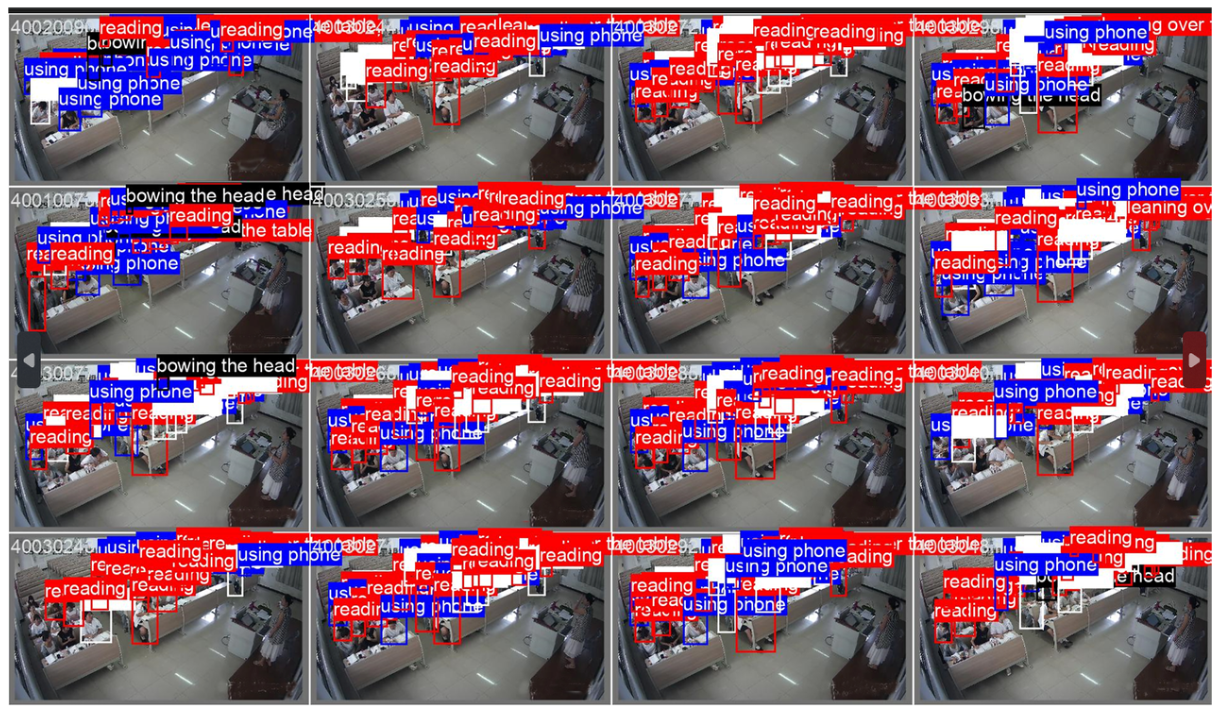
\includegraphics[width=0.9\textwidth]{figures/yolov8.png}
  \caption{Minh họa kết quả phát hiện hành vi lớp học bằng YOLOv8 kết hợp cơ chế attention. Nguồn: Zhang và cộng sự \cite{zhang2025yolov8attention}.}
  \label{fig:yolov8-mhsa-detection}
\end{figure}

Sau khi phát hiện theo khung hình, hệ thống cần duy trì sự liên tục của đối tượng qua thời gian. ByteTrack là một phương pháp multi-object tracking liên kết các hộp phát hiện thành track bằng cách tận dụng cả hộp điểm cao và hộp điểm thấp \,\cite{zhang2022bytetrack}. Trong CausClass, ByteTrack giúp biến các phát hiện rời rạc thành các đoạn sự kiện có thời gian bắt đầu--kết thúc, tạo đầu vào ổn định hơn cho bước gom time bin.


\section{Chuỗi thời gian và khám phá liên kết dự báo}
Nền tảng kỹ thuật thứ hai của CausClass là biểu diễn chuỗi thời gian và khám phá liên kết dự báo. Sau bước phát hiện và theo dõi, các sự kiện hành vi được gom vào những khoảng thời gian cố định. Việc gom theo time bin làm giảm độ nhiễu của phát hiện theo từng khung hình và đưa dữ liệu về dạng chuỗi đa biến \(X\in\mathbb{R}^{T\times K}\), trong đó \(T\) là số khoảng thời gian và \(K\) là số biến hành vi. Đây là dạng dữ liệu phù hợp hơn cho việc khảo sát các mẫu thay đổi theo thời gian.

Một trực giác quan trọng trong phân tích chuỗi thời gian là phụ thuộc trễ. Nếu một hành vi thường thay đổi trước một hành vi khác, lịch sử của hành vi thứ nhất có thể chứa thông tin hữu ích để dự báo hành vi thứ hai. Truyền thống Granger mô tả ý tưởng này bằng việc so sánh lỗi dự báo khi có và không có lịch sử của biến nguồn \,\cite{granger1969causality}, trong khi các tổng quan gần đây nhấn mạnh rằng suy luận nhân quả trên chuỗi thời gian cần phân biệt rõ dự báo, điều kiện hóa và giả định can thiệp \,\cite{runge2023causalreview}. Một liên kết dự báo từ \(i\) sang \(j\) có thể được viết dưới dạng
\begin{equation}
\label{eq:granger-predictive-link}
    i\rightarrow j
    \quad \Longleftrightarrow \quad
    \mathcal{L}\left(X_{j,t}\mid \mathcal{H}_{j,t-1},\mathcal{H}_{i,t-1}\right)
    <
    \mathcal{L}\left(X_{j,t}\mid \mathcal{H}_{j,t-1}\right),
\end{equation}
trong đó \(\mathcal{H}_{i,t-1}\) là lịch sử của biến \(i\) trước thời điểm \(t\), còn \(\mathcal{L}\) là lỗi dự báo. Cạnh \(i\rightarrow j\) vì vậy nên được hiểu là quan hệ dự báo có điều kiện trong mô hình, không phải kết luận rằng \(i\) gây ra \(j\) theo nghĩa can thiệp.

AERCA cung cấp một cách học cấu trúc dự báo trên chuỗi thời gian đa biến bằng autoencoder \,\cite{han2025aerca}. Trong mô hình gốc, encoder ước lượng thành phần ngoại sinh, còn decoder tái tạo quan sát từ lịch sử và biến ngoại sinh dưới một cấu trúc phụ thuộc học được. Thiết kế này phù hợp với dữ liệu đa biến vì nó cho phép mô hình học các phụ thuộc phi tuyến và tạo tín hiệu cấu trúc giữa các biến. Cách tiếp cận này bổ sung cho các baseline khám phá cấu trúc chuỗi thời gian đã được dùng rộng rãi như PCMCI và DYNOTEARS \,\cite{runge2019pcmci,pamfil2020dynotears}. Hình~\ref{fig:aerca-architecture} minh họa kiến trúc AERCA gốc.

\begin{figure}[H]
  \centering
  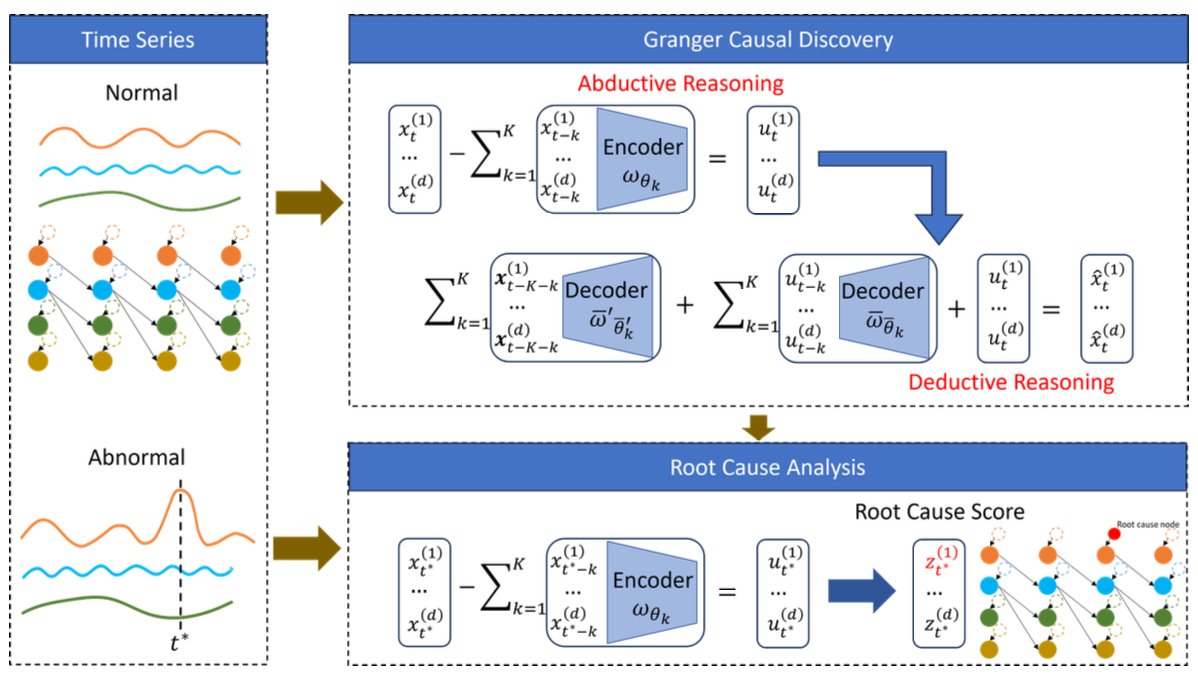
\includegraphics[width=0.9\textwidth]{figures/aerca.png}
  \caption{Minh họa cấu trúc AERCA dùng autoencoder để học phụ thuộc Granger trên chuỗi thời gian đa biến. Nguồn: Han và cộng sự \cite{han2025aerca}.}
  \label{fig:aerca-architecture}
\end{figure}

Trong CausClass, AERCA được dùng theo hai vai trò. Thứ nhất, mô hình tạo đồ thị khởi tạo và tín hiệu hệ số thô từ chuỗi hành vi. Thứ hai, AERCA có mask được dùng như bộ kiểm chứng cho các đồ thị ứng viên. Khi áp một mask cấu trúc, mô hình chỉ được phép sử dụng các liên kết nằm trong đồ thị ứng viên, từ đó đánh giá xem cấu trúc đó có đủ khả năng dự báo chuỗi \(X\) hay không.

Để tránh đồ thị quá dày, CausClass dùng điểm số kết hợp lỗi dự báo với phạt độ phức tạp. Một dạng tổng quát của điểm số là
\begin{equation}
\label{eq:graph-score}
    \mathcal{S}(G) = \mathcal{L}(X;G) + \lambda |E|,
\end{equation}
trong đó \(\mathcal{L}(X;G)\) là lỗi dự báo hoặc lỗi tái tạo khi mô hình bị ràng buộc bởi cấu trúc \(G\), \(|E|\) là số cạnh liên hành vi và \(\lambda\) là hệ số phạt độ phức tạp. Điểm số thấp hơn biểu thị ứng viên tốt hơn. Nguyên tắc này giúp đồ thị cuối cùng không chỉ khớp dữ liệu, mà còn đủ gọn để người dùng có thể kiểm tra và diễn giải.

Khi áp dụng vào dữ liệu lớp học, ba mức diễn giải cần được phân biệt rõ: tương quan đồng thời, liên kết dự báo theo thời gian và quan hệ nhân quả. Theo nền tảng suy luận nhân quả, diễn giải nhân quả đòi hỏi mô hình giả định và điều kiện nhận dạng mạnh hơn so với việc phát hiện phụ thuộc thống kê \,\cite{pearl2009causality,peters2017elements}. Dữ liệu video thụ động không có can thiệp và thường thiếu nhiều biến nền, nên đồ án chỉ sử dụng mức liên kết dự báo. Đây là lựa chọn thận trọng: đồ thị giúp người dùng xác định quan hệ thời gian đáng kiểm tra, còn kết luận sư phạm vẫn cần con người xem lại video và đặt kết quả vào bối cảnh lớp học.

\section{LLM hỗ trợ tìm kiếm và diễn giải đồ thị}
Nền tảng kỹ thuật thứ ba của CausClass là sử dụng LLM để hỗ trợ tìm kiếm và diễn giải đồ thị. LLM có khả năng xử lý mô tả biến bằng ngôn ngữ tự nhiên và khai thác tri thức miền ở mức khái quát. Trong bài toán lớp học, tri thức này có thể giúp nêu các giả thuyết như hành vi trao đổi có thể liên quan đến các hành vi tương tác khác, hoặc hành vi sử dụng điện thoại có thể tạo ra mẫu thời gian khác với đọc và viết. Tuy nhiên, các giả thuyết như vậy chỉ có giá trị nếu được kiểm chứng bằng dữ liệu quan sát.

Các nghiên cứu gần đây thường dùng LLM theo hai cách. Cách thứ nhất xem LLM như nguồn prior cấu trúc: mô hình gợi ý hướng cạnh, quan hệ hợp lý hoặc ràng buộc giữa biến, sau đó thuật toán thống kê dùng các gợi ý này để thu hẹp không gian tìm kiếm \,\cite{darvariu2024llmpriors,barakati2025llmassisted}. Cách thứ hai dùng LLM như tác nhân thăm dò đồ thị, trong đó mô hình đề xuất các bước chỉnh sửa dựa trên đồ thị hiện tại, phản hồi từ dữ liệu và mô tả nhiệm vụ \,\cite{jiralerspong2024efficient,roy2025causalllm,peng2026causcientist}. Cả hai cách đều cho thấy LLM có thể hỗ trợ tìm kiếm, nhưng không loại bỏ nhu cầu đánh giá định lượng.

Trong CausClass, LLM được đặt vào vai trò bộ sinh đề xuất. Ở mỗi vòng tìm kiếm, LLM nhận mô tả biến hành vi, đồ thị hiện tại, danh sách tabu, phản hồi từ các chỉnh sửa bị loại và tín hiệu từ AERCA, chẳng hạn các cạnh mạnh nhưng chưa được giữ trong đồ thị hiện tại. Mô hình có thể đề xuất thêm hoặc xóa một số cạnh. Sau đó, mỗi chỉnh sửa được chuyển thành đồ thị ứng viên, áp mask vào AERCA và đánh giá lại bằng lỗi kiểm chứng cùng phạt độ phức tạp. Như vậy, LLM mở rộng không gian giả thuyết, còn verifier định lượng quyết định ứng viên nào được giữ.

Chiến lược tìm kiếm được dùng là beam search. Thay vì chỉ giữ một đồ thị tốt nhất tại mỗi bước như tìm kiếm tham lam, beam search giữ một tập nhỏ các đồ thị hứa hẹn để tiếp tục mở rộng. Điều này giảm nguy cơ mắc kẹt ở một chỉnh sửa cục bộ. So với tìm kiếm ngẫu nhiên, LLM giúp ưu tiên các chỉnh sửa có ý nghĩa miền trước khi đưa vào kiểm chứng. Cơ chế này phản ánh quan điểm thiết kế của đồ án: tri thức ngữ nghĩa giúp định hướng, còn dữ liệu quyết định.

LLM cũng được dùng trong phần sinh báo cáo quan sát. Báo cáo cần chuyển thống kê chuỗi thời gian và danh sách cạnh thành văn bản dễ đọc, nhưng không được đổi chiều cạnh, phát minh cạnh mới hoặc biến liên kết dự báo thành kết luận nhân quả. Vì vậy, CausClass render xác định các phần dữ kiện như thống kê hành vi và danh sách cạnh trước, sau đó chỉ cho LLM viết các đoạn diễn giải có ràng buộc. Báo cáo phải bắt đầu từ bằng chứng phát hiện, trình bày liên kết thời gian như giả thuyết cần kiểm tra và khuyến nghị người dùng quay lại video khi cần đưa ra nhận định.

Tóm lại, Chương 2 đã trình bày ngữ cảnh bài toán, các nghiên cứu tương tự và những nền tảng kỹ thuật chính của CausClass. Các nội dung này dẫn đến thiết kế ở Chương 3: YOLO26n-MHSA đảm nhiệm perception thị giác, ByteTrack và time bin tạo chuỗi hành vi, AERCA kiểm chứng đồ thị liên kết dự báo, LLM đề xuất chỉnh sửa cấu trúc và bộ sinh báo cáo trình bày kết quả theo nguyên tắc evidence-first. Cách tổ chức này giúp hệ thống cân bằng ba yêu cầu: tự động hóa, khả năng diễn giải và sự thận trọng khi xử lý dữ liệu giáo dục quan sát.

\newpage
\chapter{PHƯƠNG PHÁP ĐỀ XUẤT}

\section{Tổng quan giải pháp}
CausClass gồm ba giai đoạn vận hành nối tiếp. Giai đoạn 1 phát hiện, theo dõi và gom hành vi lớp học từ video thành chuỗi thời gian đa biến. Giai đoạn 2 tìm kiếm đồ thị liên kết thời gian trên chuỗi đó bằng AERCA, bộ sinh đề xuất LLM và beam search. Giai đoạn 3 chuyển tóm tắt chuỗi thời gian và các cạnh đồ thị đã kiểm chứng thành báo cáo quan sát theo nguyên tắc evidence-first. Báo cáo bị ràng buộc có chủ đích: phải nêu dữ kiện phát hiện trước, diễn giải cạnh đồ thị một cách thận trọng và khuyến nghị con người kiểm tra lại video trước mọi hành động trong lớp học.

\begin{figure}[htbp]
  \centering
  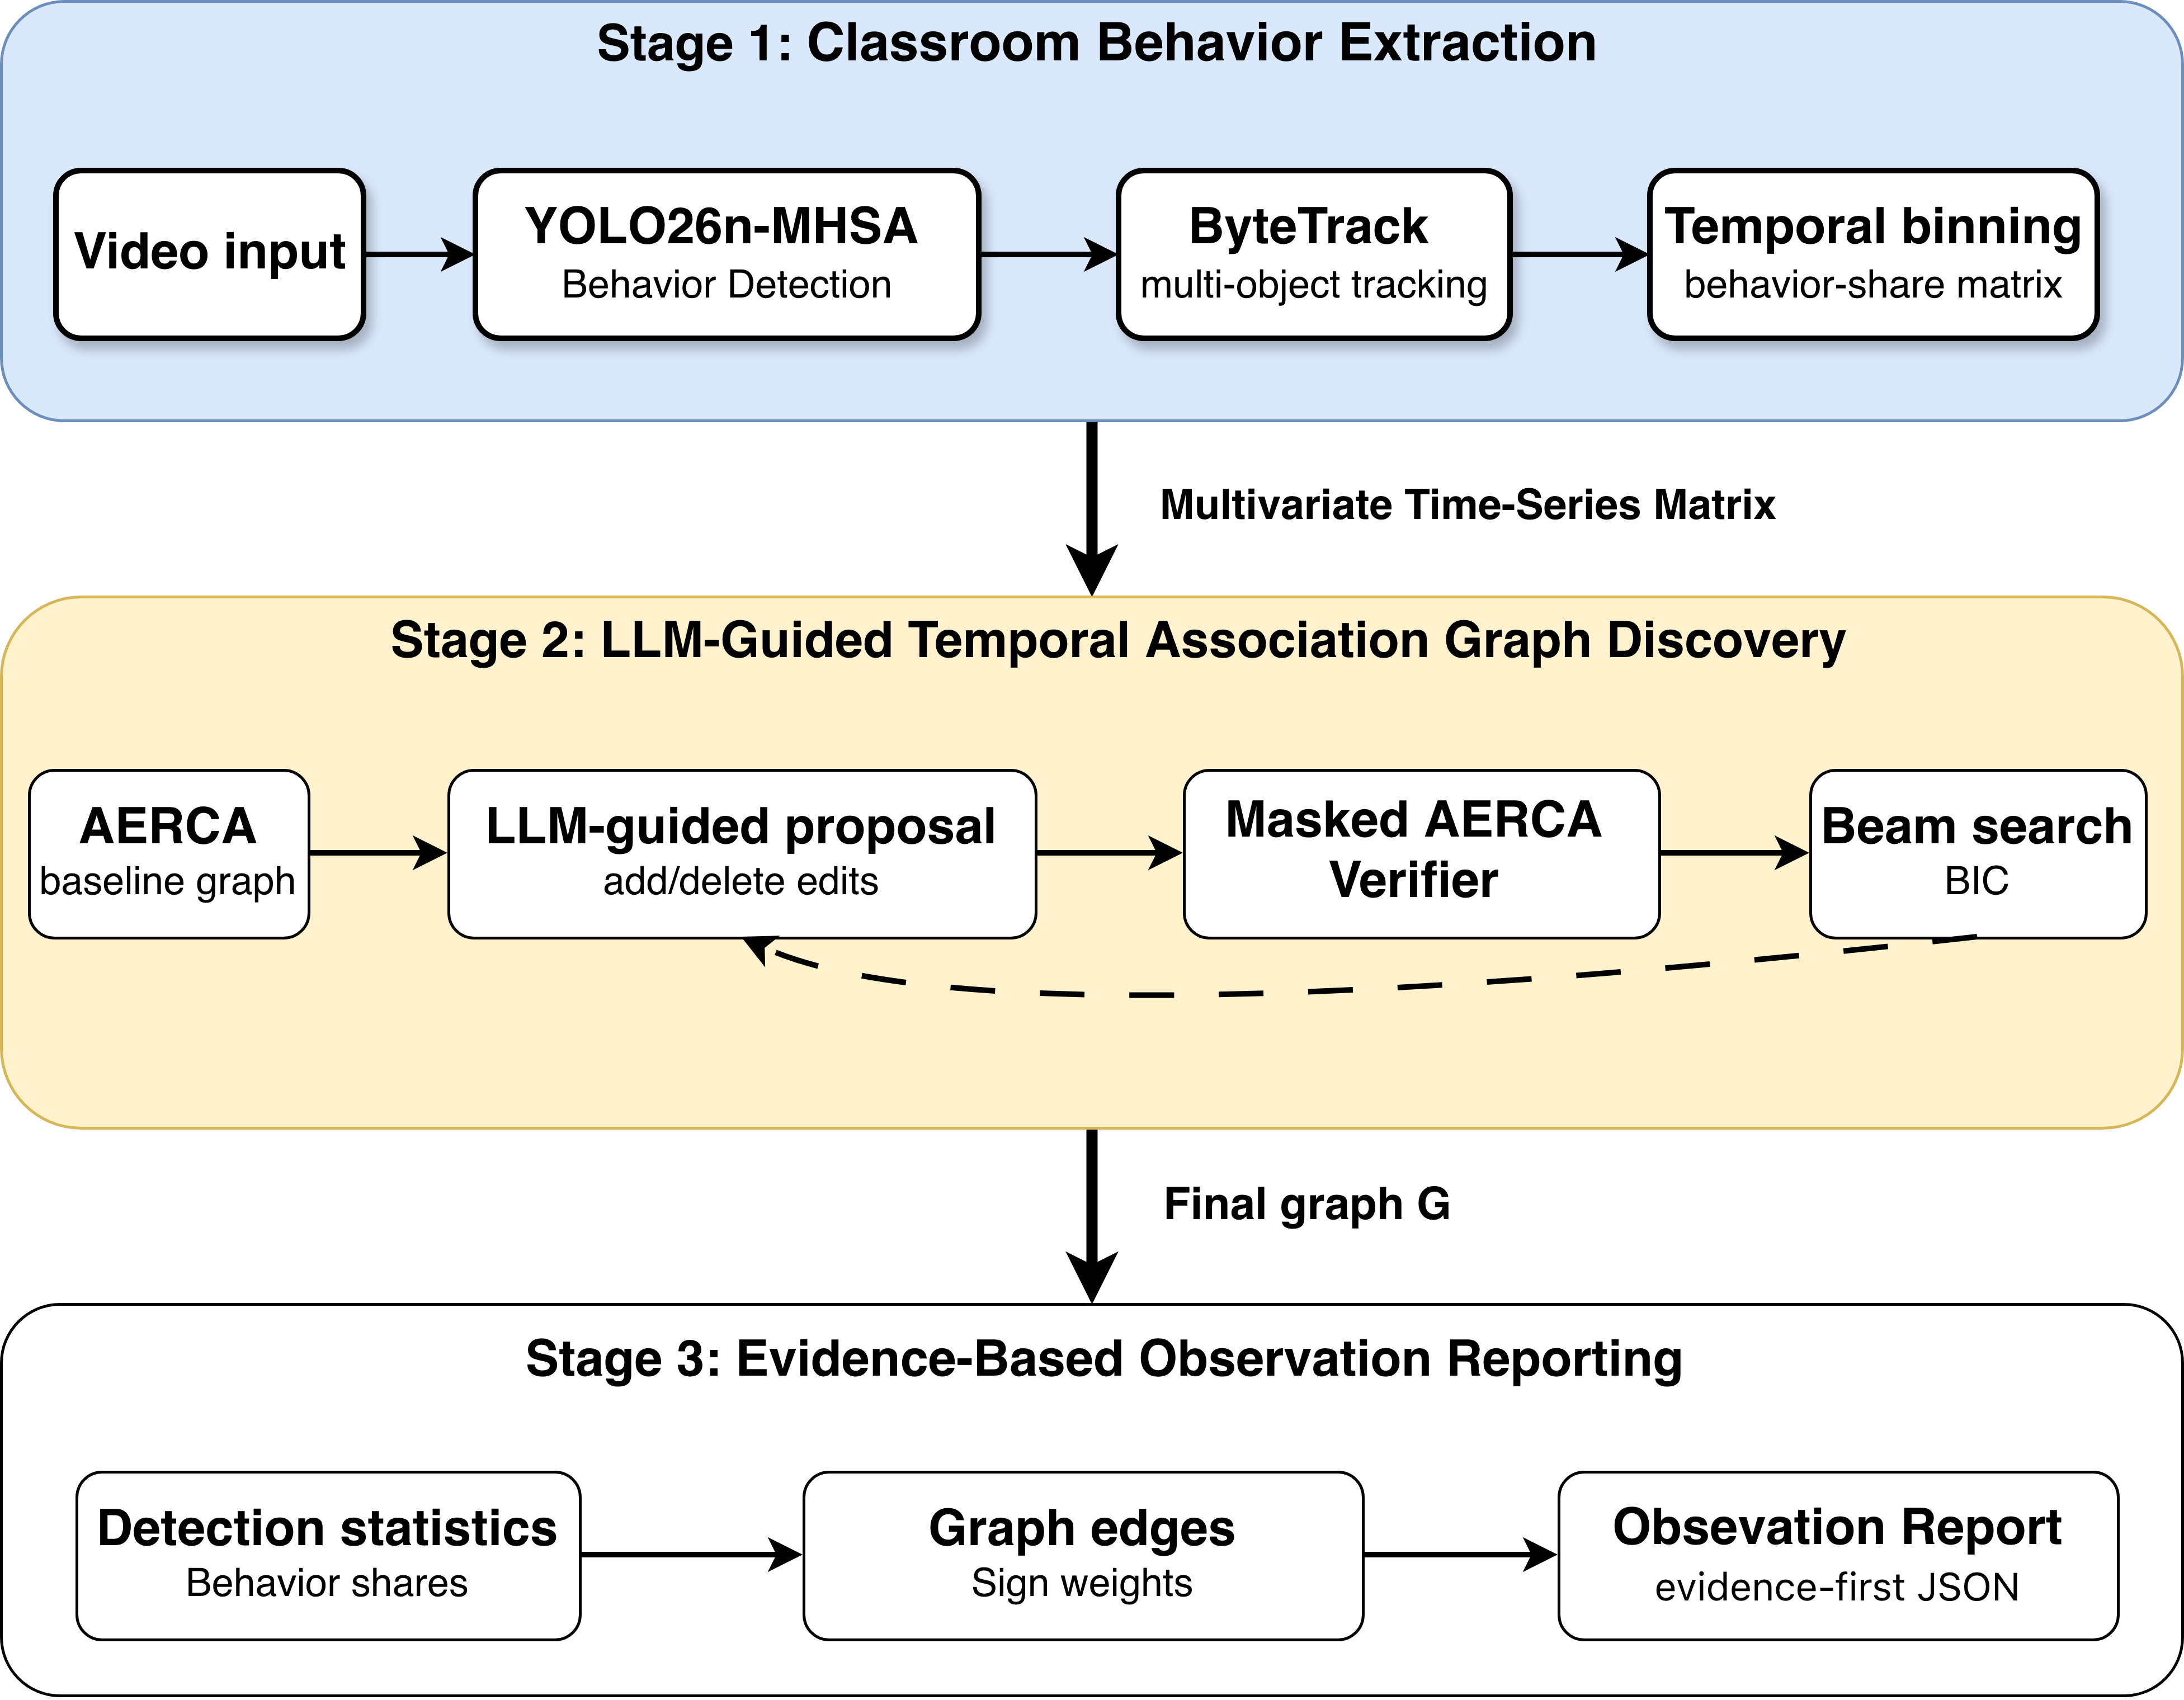
\includegraphics[width=0.95\textwidth]{figures/overall.png}
  \caption{Tổng quan pipeline CausClass. Hệ thống được chia thành ba giai đoạn: trích xuất chuỗi thời gian hành vi từ video, khám phá liên kết thời gian và sinh báo cáo quan sát dựa trên bằng chứng.}
  \label{fig:causclass-overview}
\end{figure}

Hình~\ref{fig:causclass-overview} tóm tắt luồng dữ liệu của toàn hệ thống. Sự tách biệt giữa các giai đoạn là một cơ chế an toàn quan trọng. Phát hiện và theo dõi chỉ tạo bằng chứng quan sát; tìm kiếm đồ thị chỉ tóm tắt cấu trúc dự báo theo thời gian; sinh báo cáo chỉ chuyển các bằng chứng đã có thành văn bản dễ đọc. Không giai đoạn nào được phép tự nâng cấp liên kết quan sát thành kết luận nhân quả chắc chắn hoặc kết luận sư phạm cuối cùng.

Luồng dữ liệu chính có thể viết dưới dạng
\begin{equation}
\label{eq:causclass-pipeline}
    V \rightarrow \mathcal{E} \rightarrow X \rightarrow G^\star \rightarrow R,
\end{equation}
trong đó \(V\) là video đầu vào, \(\mathcal{E}\) là tập sự kiện hành vi sau phát hiện và theo dõi, \(X\in\mathbb{R}^{T\times K}\) là chuỗi thời gian hành vi gồm \(T\) time bin và \(K\) biến hành vi, \(G^\star\) là đồ thị liên kết thời gian cuối cùng và \(R\) là báo cáo quan sát. Mỗi mũi tên là một phép biến đổi có artifact trung gian: khung debug, file sự kiện vi mô, CSV chuỗi thời gian, danh sách cạnh, ma trận kề và báo cáo. Thiết kế này giúp truy vết lỗi: nếu báo cáo có nhận xét bất thường, người dùng có thể quay lại cạnh đồ thị, chuỗi thời gian, sự kiện phát hiện hoặc khung hình gốc.

Trong giai đoạn perception và temporal abstraction, detector YOLO26n-MHSA tạo các hộp phát hiện hành vi theo từng khung hình. ByteTrack liên kết các hộp này thành track để giảm đứt đoạn ngắn và tạo sự kiện có thời gian bắt đầu--kết thúc; các sự kiện sau đó được gom theo time bin thành tỉ lệ hành vi. Trong giai đoạn temporal discovery, AERCA cung cấp đồ thị ban đầu và tín hiệu hệ số. LLM không trực tiếp quyết định đồ thị; nó chỉ đề xuất chỉnh sửa, còn masked AERCA và điểm số BIC-style đánh giá ứng viên. Trong giai đoạn reporting, đồ thị đã kiểm chứng và tóm tắt chuỗi thời gian được render thành báo cáo có ràng buộc, không cho phép đổi chiều cạnh hoặc phát minh quan hệ mới.

Nguyên tắc thiết kế xuyên suốt là phân tách vai trò giữa quan sát, kiểm chứng và diễn giải. Detector trả lời câu hỏi ``hành vi nào được nhìn thấy''. Mô hình thời gian trả lời câu hỏi ``tín hiệu nào có ích cho dự báo tín hiệu nào''. Báo cáo trả lời câu hỏi ``người dùng nên kiểm tra điều gì trong video''. Nhờ phân tách này, CausClass phù hợp với dữ liệu lớp học quan sát thụ động: hệ thống hỗ trợ phân tích và đặt giả thuyết, nhưng không thay thế chuyên gia giáo dục trong việc xác định ý nghĩa sư phạm.

\section{Kiến trúc YOLO26n-MHSA}
YOLO26n-MHSA được dẫn xuất từ YOLO26n bằng một thay đổi cục bộ trong đường tổng hợp đặc trưng, thay vì thiết kế lại toàn bộ detector. Kiến trúc YOLO26n gốc chủ yếu dựa trên các khối tích chập để trích xuất mẫu thị giác cục bộ và hợp nhất đặc trưng đa tỉ lệ trước lớp \textit{Detect}. Thiết kế này hiệu quả về tính toán, nhưng hành vi trong lớp học thường phụ thuộc vào quan hệ không gian xa, ví dụ tương quan giữa tư thế đầu, vị trí tay, vùng bàn học và vật thể nhỏ như điện thoại hoặc vở.

\begin{figure}[htbp]
  \centering
  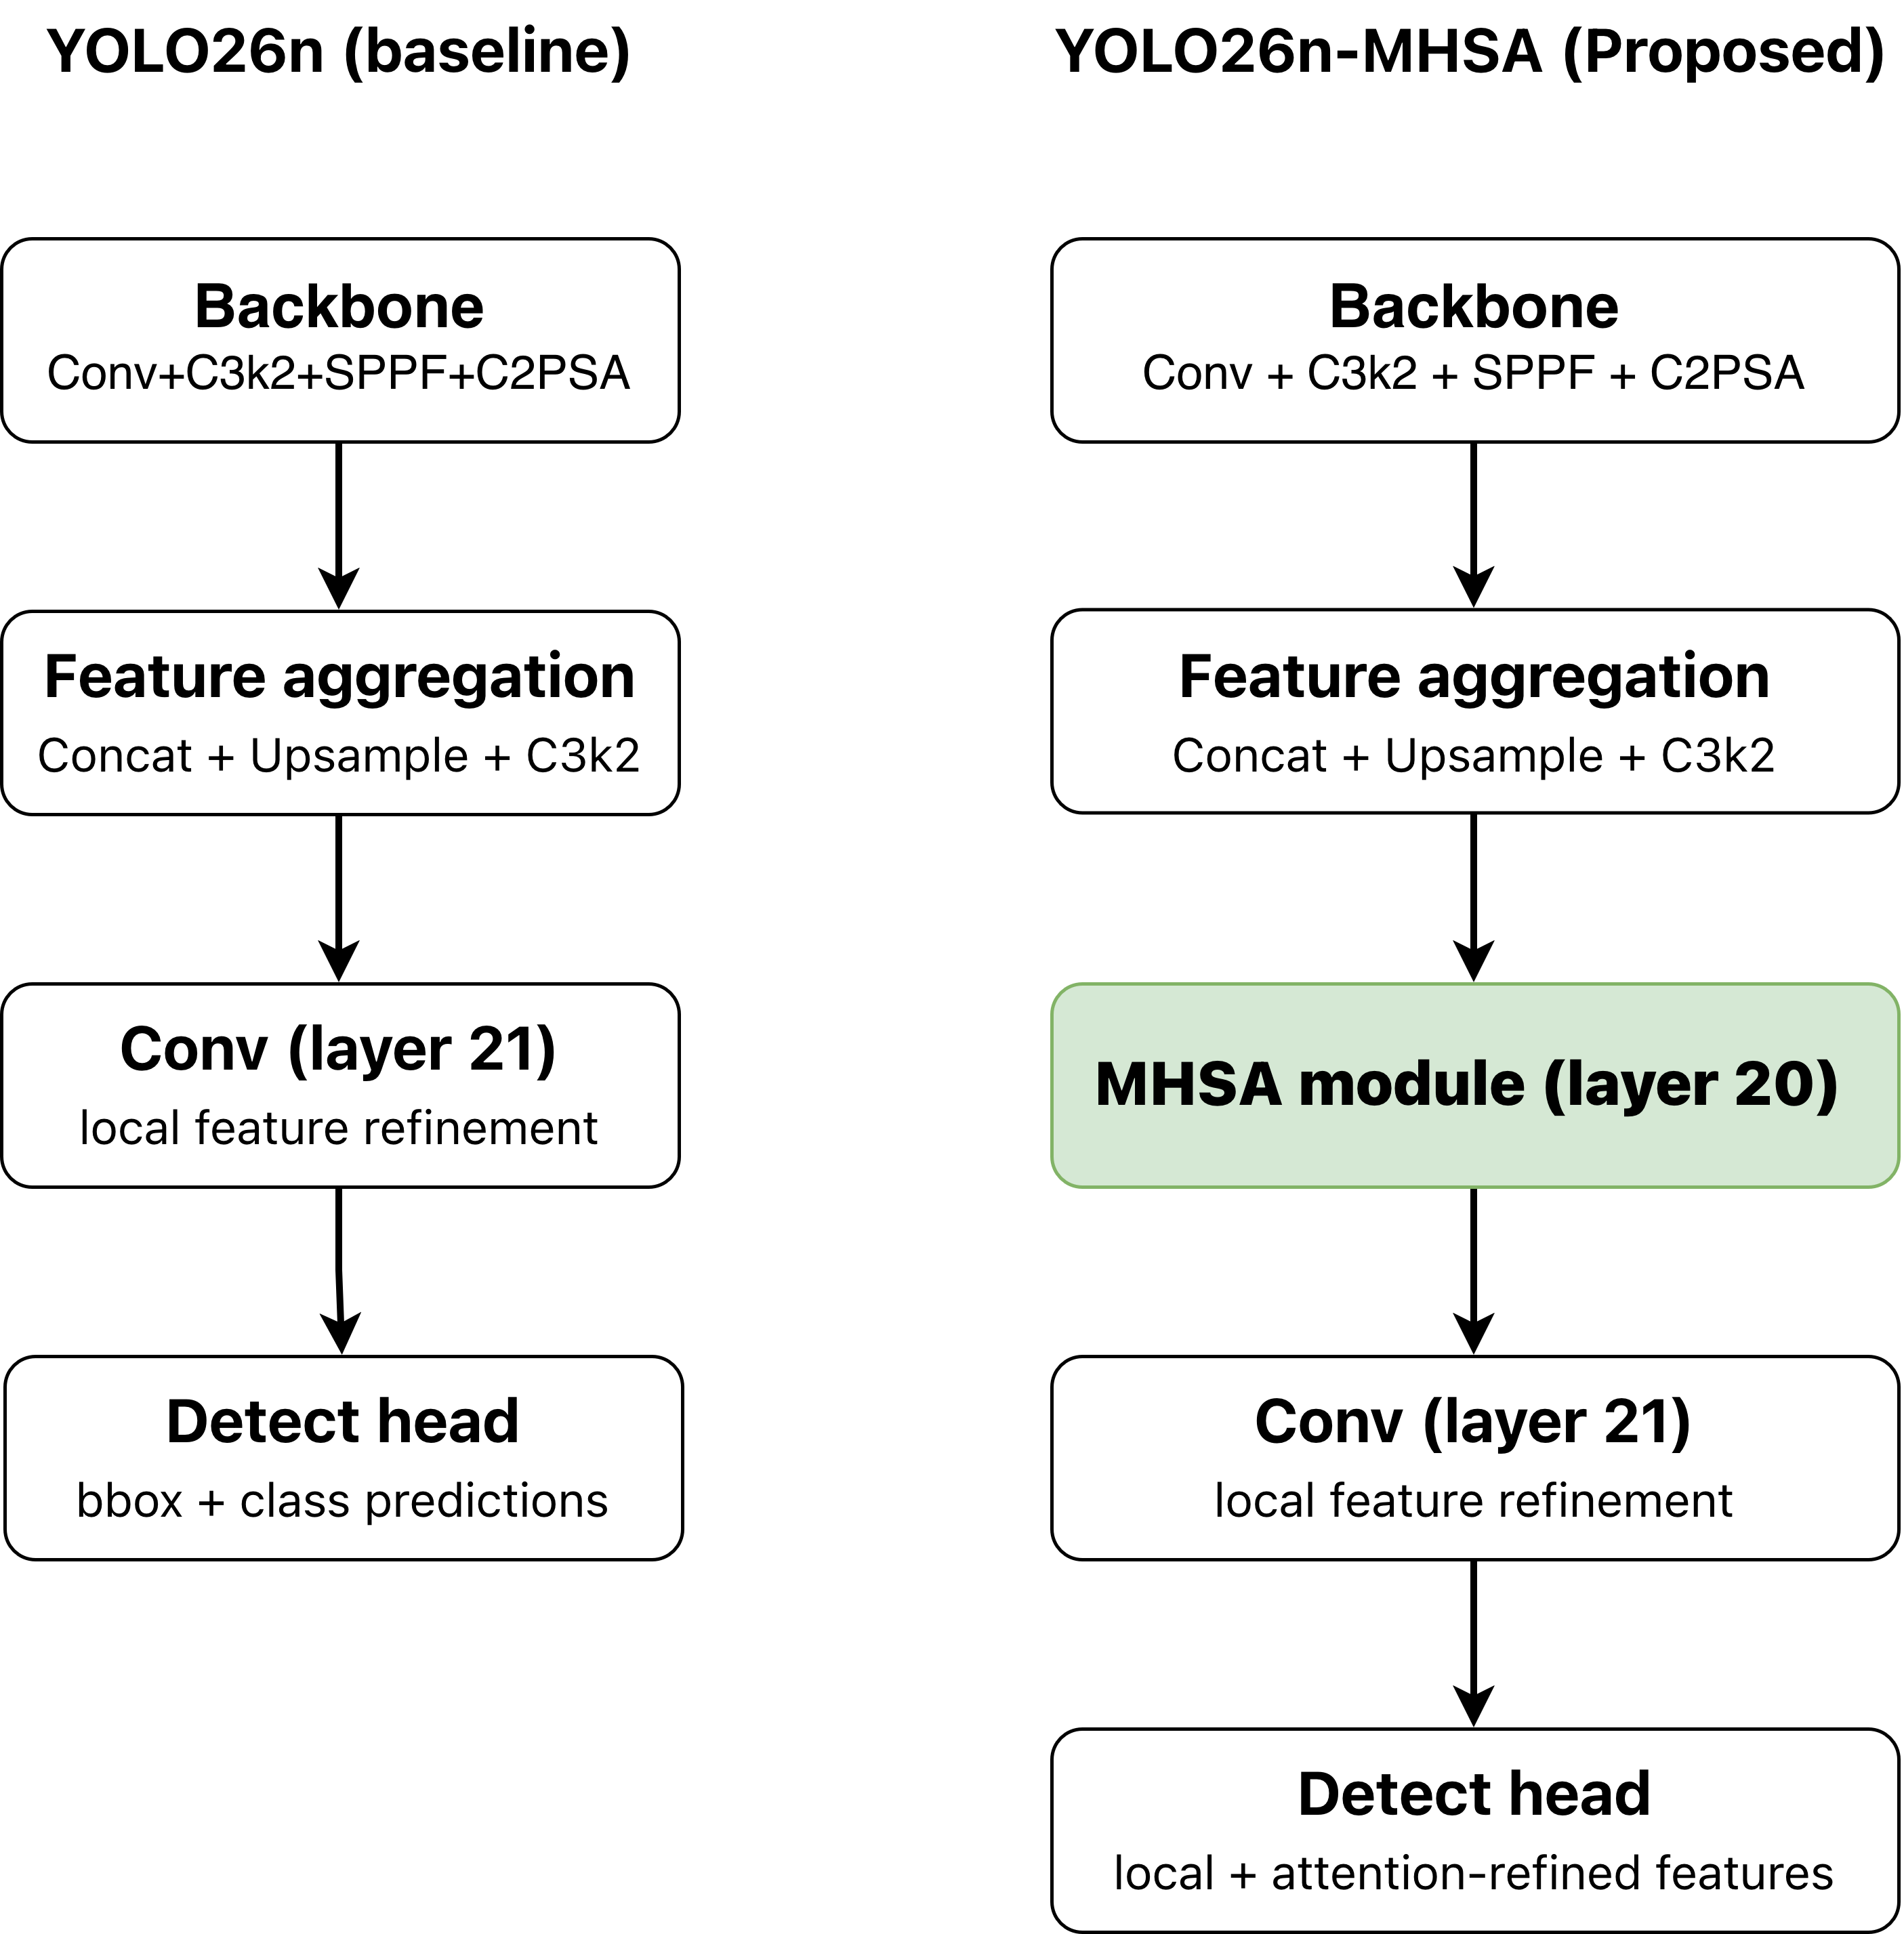
\includegraphics[width=0.9\textwidth]{figures/yolo.png}
  \caption{So sánh cấu trúc giữa detector YOLO26n gốc và biến thể YOLO26n-MHSA. Biến thể đề xuất chèn một khối MHSA vào head phát hiện để bổ sung ngữ cảnh không cục bộ trước lớp phát hiện cuối.}
  \label{fig:yolo-mhsa}
\end{figure}

Hình~\ref{fig:yolo-mhsa} trình bày khác biệt cấu trúc trước và sau khi thêm Multi-Head Self-Attention. Trong YOLO26n-MHSA, backbone và hầu hết kết nối trong head phát hiện được giữ nguyên. Thay đổi chính là chèn một khối MHSA sau khối C3k2 tại layer 19 và trước lớp tích chập tiếp theo tại layer 21. Nhánh đặc trưng đã tăng cường attention sau đó tiếp tục được đưa tới lớp \textit{Detect} cùng các đặc trưng ở tỉ lệ khác. Cách đặt này cho phép detector tinh chỉnh một nhánh đặc trưng trung gian bằng ngữ cảnh toàn cục nhưng vẫn giữ luồng đặc trưng YOLO đa tỉ lệ và backbone nhẹ. Cấu hình YAML đầy đủ của biến thể này được trình bày trong Phụ lục~\ref{appendix:yolo26n-mhsa-yaml}.

Lý do chọn thay đổi cục bộ là để giữ thí nghiệm so sánh có kiểm soát. Nếu thay đổi đồng thời backbone, neck, head và chiến lược huấn luyện, rất khó xác định phần cải thiện đến từ đâu. Trong thiết kế này, phần lớn kiến trúc YOLO26n được giữ nguyên; do đó khác biệt hiệu năng giữa YOLO26n và YOLO26n-MHSA có thể quy chủ yếu cho mô-đun MHSA được thêm vào. Điều này phù hợp với mục tiêu của đồ án: khảo sát vai trò của attention đối với nhận diện hành vi lớp học trong bối cảnh nhiều đối tượng và nhiều che khuất.

Gọi \(F\in\mathbb{R}^{H\times W\times C}\) là bản đồ đặc trưng đi vào mô-đun MHSA, trong đó \(H\), \(W\) và \(C\) lần lượt là chiều cao, chiều rộng và số kênh. Bản đồ đặc trưng được làm phẳng thành chuỗi token
\begin{equation}
\label{eq:mhsa-flattened-features}
    Z\in\mathbb{R}^{N\times C}, \qquad N=H\times W.
\end{equation}
Từ \(Z\), mô-đun tính các ma trận query, key và value:
\begin{equation}
\label{eq:mhsa-projections}
    Q=ZW_Q, \qquad K=ZW_K, \qquad V=ZW_V.
\end{equation}
Với một attention head, scaled dot-product attention được tính bởi
\begin{equation}
\label{eq:scaled-dot-product-attention}
    \operatorname{Attention}(Q,K,V)=\operatorname{softmax}\left(\frac{QK^\top}{\sqrt{d}}\right)V,
\end{equation}
trong đó \(d\) là chiều của vector query và key. Với \(h\) head song song, đầu ra của các head được ghép và chiếu tuyến tính:
\begin{equation}
\label{eq:mhsa-output}
    \operatorname{MHSA}(Z)=\operatorname{Concat}(head_1,head_2,\ldots,head_h)W_O.
\end{equation}
Một kết nối tắt được dùng để bảo toàn biểu diễn ban đầu:
\begin{equation}
\label{eq:mhsa-residual}
    Z' = Z + \operatorname{MHSA}(Z).
\end{equation}
Sau đó \(Z'\) được reshape lại thành bản đồ đặc trưng không gian và truyền tới các lớp còn lại của head.

Về mặt trực giác, MHSA cho phép một vị trí đặc trưng ở vùng đầu, tay hoặc bàn học trao đổi thông tin với các vùng xa hơn trước khi detector dự đoán hộp và nhãn. Điều này đặc biệt hữu ích với các hành vi có tín hiệu phân tán, chẳng hạn viết bài phụ thuộc vào cả tư thế tay và vùng vở, hoặc sử dụng điện thoại phụ thuộc vào vật thể nhỏ trong tay và tư thế nhìn xuống. Tuy nhiên, vì chỉ thêm một nhánh attention, mô hình vẫn giữ được tính nhẹ của YOLO26n và phù hợp với pipeline video.

Đầu ra của YOLO26n-MHSA ở mỗi khung hình là tập hộp phát hiện kèm nhãn hành vi và điểm tin cậy. Các nhãn này được giữ thống nhất trong toàn pipeline; việc ánh xạ nhãn giữa bộ dữ liệu Local và SCB chỉ được thực hiện trong thiết lập thực nghiệm. Phần method vì vậy xem detector như nguồn tạo bằng chứng quan sát, còn mọi diễn giải phía sau phải tính đến khả năng detector bỏ sót hoặc nhận nhầm hành vi.

\section{Theo dõi và xây dựng chuỗi thời gian}
Đối với suy luận trên video thật, detector được kết hợp với ByteTrack. ByteTrack liên kết các phát hiện qua khung hình, bao gồm cả một số hộp có độ tin cậy thấp, nhờ đó giúp duy trì quỹ đạo đối tượng trong cảnh đông người và nhiều che khuất \,\cite{zhang2022bytetrack}. Khi một đoạn track kết thúc, pipeline lưu nó thành một sự kiện vi mô chứa định danh đối tượng, nhãn hành vi, thời gian bắt đầu, thời gian kết thúc và thông tin độ tin cậy.

Một sự kiện vi mô có thể viết dưới dạng
\begin{equation}
\label{eq:tracked-event}
    e=(u,b,t_a,t_b,\bar{s}),
\end{equation}
trong đó \(u\) là định danh track, \(b\) là nhãn hành vi, \([t_a,t_b]\) là khoảng thời gian sự kiện và \(\bar{s}\) là điểm tin cậy trung bình của các phát hiện thuộc sự kiện. Cách biểu diễn sự kiện theo đoạn thời gian giảm nhiễu so với đếm từng khung hình độc lập, đặc biệt khi video có FPS cao hoặc khi detector dao động nhẹ giữa các khung hình liên tiếp.

Các sự kiện vi mô được gom vào các time bin có độ rộng cố định. Với time bin \(r\) và hành vi \(k\), tỉ lệ hành vi trong pipeline được tính là
\begin{equation}
\label{eq:time-bin-percentage}
    X_{r,k}=100\times\frac{N_{r,k}}{\sum_{j=1}^{K}N_{r,j}},
\end{equation}
trong đó \(N_{r,k}\) là số sự kiện track của hành vi \(k\) chồng lấn với bin \(r\), và \(K\) là số hành vi được xét. Nếu trong một bin không có phát hiện nào, toàn bộ tỉ lệ hành vi của bin đó được đặt bằng 0. Các giá trị này là phần trăm của sự kiện hành vi được detector ghi nhận, không phải phần trăm chính xác số học sinh thật sự thực hiện hành vi trong lớp.

Nếu xét toàn bộ video gồm \(T\) time bin, Stage 1 sinh ra ma trận chuỗi thời gian
\begin{equation}
\label{eq:time-series-matrix}
    X\in\mathbb{R}^{T\times K}.
\end{equation}
Mỗi hàng là một lát cắt thời gian; mỗi cột là một nhãn hành vi. Chuỗi này giữ độ dài cố định theo video và là đầu vào trực tiếp cho Stage 2. Khi cần giảm ảnh hưởng của khác biệt tần suất giữa nhãn, có thể chuẩn hóa từng biến theo dạng
\begin{equation}
\label{eq:standardized-time-series}
    \widetilde{X}_{t,k}=\frac{X_{t,k}-\mu_k}{\sigma_k+\epsilon},
\end{equation}
trong đó \(\mu_k\) và \(\sigma_k\) là trung bình và độ lệch chuẩn của hành vi \(k\), còn \(\epsilon\) là hằng số nhỏ để tránh chia cho 0. Tuy nhiên, chuỗi báo cáo cho người dùng vẫn được diễn giải trên thang phần trăm sự kiện phát hiện để dễ hiểu.

Trong triển khai, Stage 1 lưu nhiều artifact trung gian để phục vụ kiểm toán, chẳng hạn khung debug, file sự kiện vi mô, chuỗi thời gian thô và metadata video. Các tham số cụ thể của bước suy luận, theo dõi và gom bin được trình bày trong Chương 4 cùng với thiết lập thực nghiệm. Nếu một cạnh đồ thị hoặc một câu trong báo cáo có vẻ bất thường, người dùng có thể kiểm tra liệu nó xuất phát từ mẫu phát hiện thật, từ nhiễu detector, hay từ cách gom sự kiện vào bin.

Điểm cần nhấn mạnh là Stage 1 không tạo dữ liệu ``đúng tuyệt đối'' về hành vi lớp học. Chuỗi \(X\) là quan sát bị nhiễu qua detector và tracker. Nếu detector bỏ sót một hành vi, tần suất tương ứng trong \(X\) sẽ bị giảm; nếu detector phát hiện trùng hoặc sai nhãn, \(X\) sẽ chứa nhiễu. Vì vậy, các giai đoạn đồ thị và báo cáo phải được đọc như phân tích trên tín hiệu quan sát tự động, không phải trên ground truth hành vi của toàn lớp.

\section{Trích xuất đồ thị baseline bằng AERCA}
Gọi \(\mathcal{B}\) là tập biến hành vi trong đồ thị, \(K=|\mathcal{B}|\), và \(X\in\mathbb{R}^{T\times K}\) là chuỗi thời gian đa biến trên các biến này. AERCA ban đầu là một phương pháp encoder--decoder cho khám phá Granger và phân tích nguyên nhân gốc trong chuỗi thời gian đa biến \,\cite{han2025aerca}. Encoder ước lượng các thành phần ngoại sinh, còn decoder tái tạo quan sát từ lịch sử quan sát và biến ngoại sinh dưới một cấu trúc phụ thuộc học được. Trong CausClass, AERCA không được dùng chủ yếu cho định vị bất thường; nó được điều chỉnh thành một mô-đun trích xuất và kiểm chứng đồ thị.

Ở bước baseline, một mô hình AERCA dày được huấn luyện trên chuỗi hành vi. Từ mô hình đã học, pipeline trích xuất tensor hệ số thời gian và tóm tắt thành hai ma trận: ma trận hệ số median theo trị tuyệt đối để phát hiện cấu trúc cạnh, và ma trận hệ số mean có dấu để xác định dấu/trọng số của cạnh. Self-loop được loại khỏi đồ thị báo cáo ban đầu, nhưng lịch sử tự thân của mỗi biến vẫn được phép sử dụng bên trong mô hình khi kiểm chứng có mask. Cấu hình huấn luyện cụ thể của AERCA được trình bày trong Chương 4.

Đồ thị baseline được lấy bằng cách ngưỡng hóa ma trận cấu trúc thô theo quantile \(q\). Nếu ký hiệu ma trận độ mạnh liên kết là \(W\in\mathbb{R}^{K\times K}\) và \(\tau_q\) là ngưỡng quantile mức \(q\) của các phần tử ngoài đường chéo trong \(W\), đồ thị khởi tạo có ma trận kề
\begin{equation}
\label{eq:aerca-initial-adjacency}
    A^{(0)}_{ij}=\mathbf{1}\{W_{ij}\geq \tau_q\}, \qquad A^{(0)}_{ii}=0.
\end{equation}
Mỗi cạnh được giữ lại nhận dấu và trọng số từ ma trận hệ số có dấu. Đồ thị này đóng vai trò điểm xuất phát cho tìm kiếm, không phải kết quả cuối cùng bắt buộc. Giá trị ngưỡng được dùng trong từng thí nghiệm được nêu ở Chương 4.

Để kiểm chứng một đồ thị ứng viên \(G=(\mathcal{B},E)\) trên cùng tập biến hành vi, pipeline xây dựng mask nhị phân
\begin{equation}
\label{eq:graph-mask-space}
    M_G\in\{0,1\}^{K\times K},
\end{equation}
trong đó kích thước \(K\times K\) xuất phát từ \(K=|\mathcal{B}|\): mỗi hàng và mỗi cột tương ứng với một biến hành vi trong \(\mathcal{B}\). Cụ thể,
\begin{equation}
\label{eq:graph-mask-definition}
    (M_G)_{ij}=\begin{cases}
        1, & \text{nếu } (i,j)\in E,\\
        0, & \text{nếu } (i,j)\notin E.
    \end{cases}
\end{equation}
Đường chéo được đặt bằng 1,
\begin{equation}
\label{eq:self-connection-mask}
    (M_G)_{ii}=1,
\end{equation}
để mỗi biến vẫn được phép dùng lịch sử của chính nó trong dự báo. Mask không biểu diễn trọng số cạnh; nó chỉ biểu diễn ràng buộc cấu trúc: cạnh nào được phép ảnh hưởng tới dự báo và cạnh nào bị chặn.

Gọi \(\Theta\) là tập tham số của AERCA và \(C_\Theta(X)\in\mathbb{R}^{K\times K}\) là ma trận hệ số liên kết mà mô hình sử dụng sau khi thu gọn các chiều phụ. Khi áp mask của đồ thị ứng viên, hệ số hiệu dụng là
\begin{equation}
\label{eq:masked-causal-score}
    \widetilde{C}_{\Theta,G}(X)=C_\Theta(X)\odot M_G,
\end{equation}
trong đó \(\odot\) là phép nhân từng phần tử. Nếu \((M_G)_{ij}=0\), liên kết từ biến \(i\) sang biến \(j\) bị triệt tiêu trong mô hình dự báo; nếu \((M_G)_{ij}=1\), liên kết đó được phép tham gia dự báo và được tối ưu cùng các tham số còn lại.

Với mask \(M_G\), bài toán huấn luyện AERCA cho đồ thị ứng viên được viết tổng quát là
\begin{equation}
\label{eq:masked-aerca-objective}
    \Theta_G^{\star}=\arg\min_{\Theta}\;\mathcal{L}_{AERCA}(X;\Theta,M_G).
\end{equation}
Hai đồ thị khác nhau tương ứng với hai không gian mô hình khác nhau:
\begin{equation}
\label{eq:graph-mask-injectivity}
    G_a\neq G_b \quad \Rightarrow \quad M_{G_a}\neq M_{G_b}.
\end{equation}
Do đó, so sánh hai đồ thị không chỉ là so sánh hai danh sách cạnh, mà là so sánh hai mô hình AERCA được fine-tune dưới hai ràng buộc cấu trúc khác nhau.

Sau khi tối ưu dưới mask \(M_G\), đồ thị ứng viên được đánh giá bằng lỗi dự báo trên tập validation:
\begin{equation}
\label{eq:validation-mse}
    \mathrm{MSE}(G)=\frac{1}{T_{val}}\sum_{t\in\mathcal{T}_{val}}\left\|X_t-\hat{X}^{(G)}_t\right\|_2^2,
\end{equation}
trong đó \(\hat{X}^{(G)}_t\) là dự báo của AERCA khi bị ràng buộc bởi mask \(M_G\), \(\mathcal{T}_{val}\) là tập chỉ số kiểm chứng và \(T_{val}=|\mathcal{T}_{val}|\). MSE đo mức độ phù hợp dự báo của cấu trúc ứng viên, nhưng nếu chỉ tối thiểu hóa MSE, đồ thị dày có thể được ưu tiên vì có nhiều bậc tự do hơn.

Vì vậy, CausClass dùng điểm số BIC-style để cân bằng lỗi dự báo và độ phức tạp. Với \(n\) mẫu thời gian, \(|E|\) cạnh liên hành vi và hệ số phạt cạnh \(\lambda\), đồ án sử dụng
\begin{equation}
\label{eq:bic-star}
    \mathrm{BIC}^{\star}=n\log(\mathrm{MSE}+\epsilon)+\lambda |E|\log n.
\end{equation}
Điểm số này mang tính BIC-style chứ không khẳng định là BIC thống kê chính xác cho mô hình nơ-ron. Vai trò của nó là chọn đồ thị vừa dự báo tốt vừa đủ gọn để diễn giải.

Với một thao tác thêm một cạnh, ứng viên chỉ đáng được ưu tiên khi mức giảm MSE đủ trả cho phạt độ phức tạp mới:
\begin{equation}
\label{eq:bic-improvement}
    n\log\left(\frac{\mathrm{MSE}_{old}}{\mathrm{MSE}_{new}}\right)>\lambda\log n.
\end{equation}
Ngược lại, khi xóa một cạnh, đồ thị có thể chấp nhận MSE tăng nhẹ nếu phần giảm độ phức tạp bù lại. Nguyên tắc này làm cho đồ thị cuối cùng không chỉ là đồ thị khớp dữ liệu nhất, mà là đồ thị có đánh đổi hợp lý giữa dự báo và khả năng kiểm tra.

Khi áp dụng cùng nguyên tắc phạt cạnh cho các chuỗi có độ dài khác nhau, hệ số \(\lambda\) được chọn trong phần thiết lập thực nghiệm để giữ cân bằng giữa độ khớp dự báo và độ thưa của đồ thị. Cách chọn giá trị cụ thể được báo cáo ở Chương 4.

Nhờ cơ chế mask và điểm số này, AERCA trong CausClass vừa cung cấp tín hiệu cấu trúc ban đầu vừa đóng vai trò verifier cho các đồ thị do tìm kiếm sinh ra. Đây là điểm khác biệt so với việc dùng AERCA một lần rồi nhận trực tiếp đồ thị thô: mọi chỉnh sửa đồ thị đều phải được kiểm tra lại dưới cùng nguyên tắc dự báo và phạt độ phức tạp.

\section{Tìm kiếm beam có hướng dẫn bởi LLM}
AERCA có thể khôi phục nhiều phụ thuộc liên quan, nhưng đồ thị thô thường dày hoặc chứa các liên kết khó diễn giải về mặt hành vi. Vì vậy, CausClass dùng LLM như một bộ sinh đề xuất trong quá trình tìm kiếm đồ thị. Về mặt phương pháp, LLM chỉ đóng vai trò đề xuất chỉnh sửa cấu trúc dựa trên mô tả biến, đồ thị hiện tại, phản hồi từ các lần thử trước và tín hiệu hệ số thô; nó không được quyết định đồ thị cuối cùng. Các lựa chọn mô hình cụ thể và cấu hình chạy được trình bày trong Chương 4.

\begin{figure}[htbp]
  \centering
  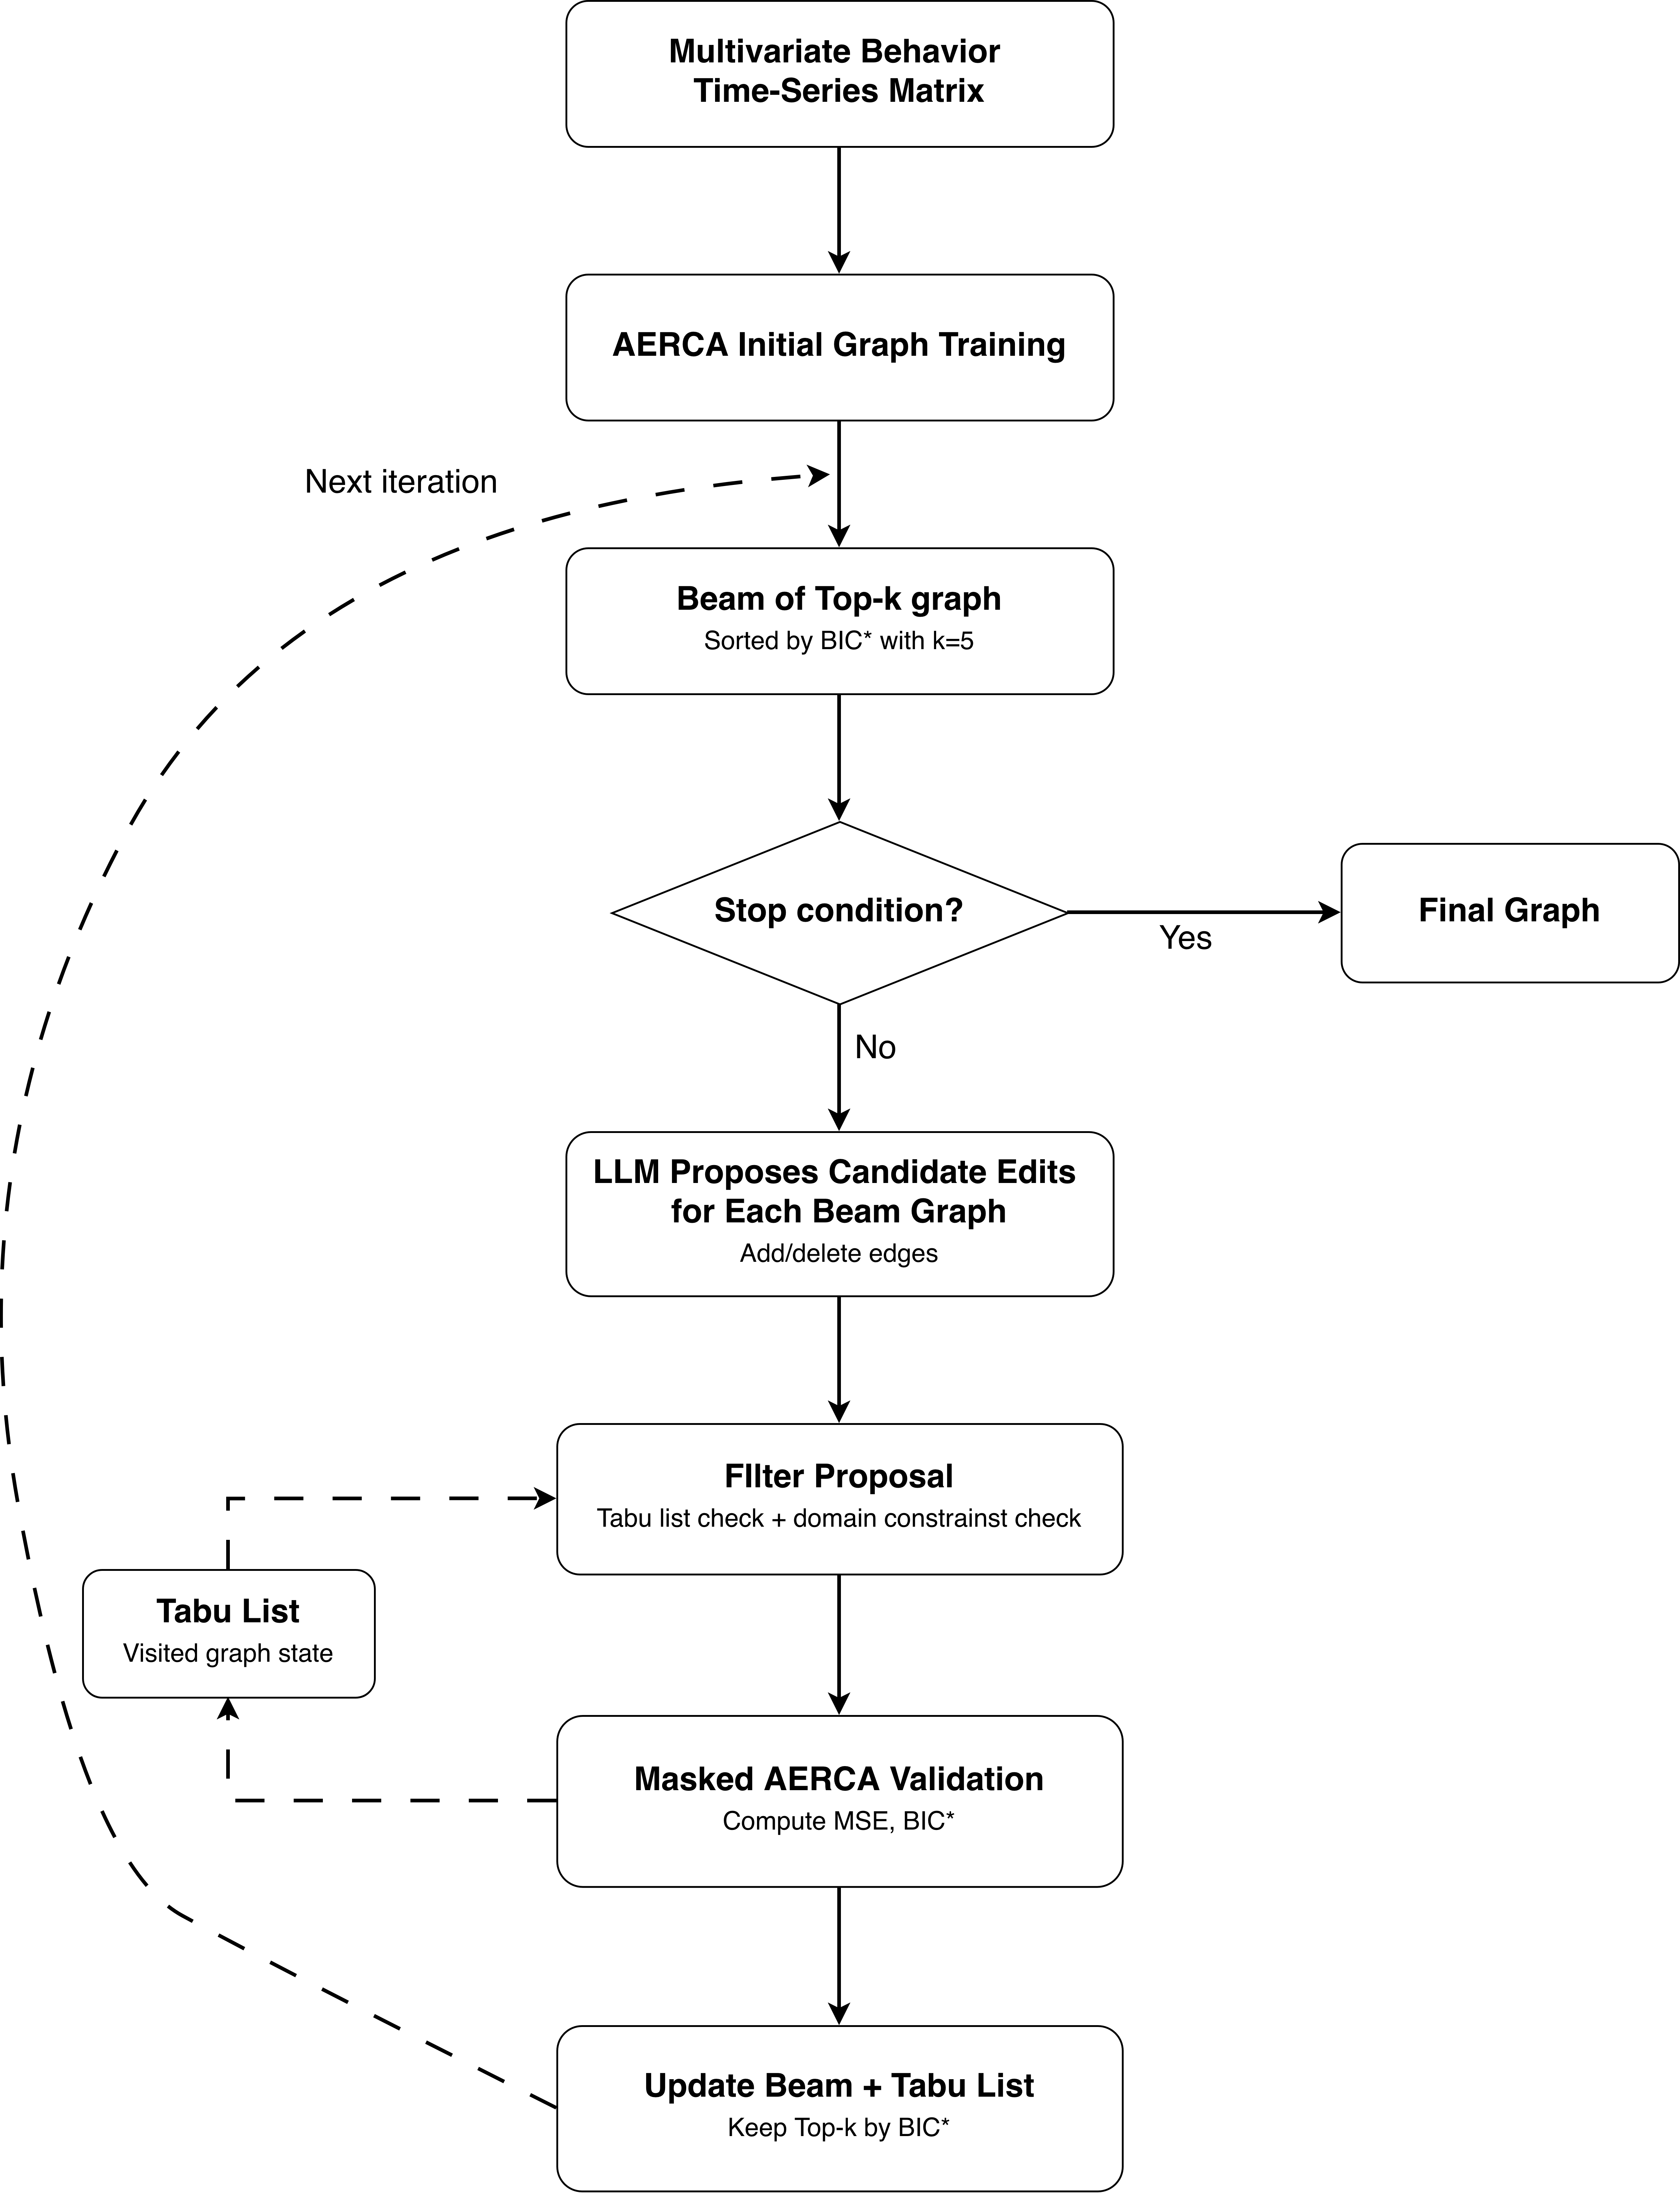
\includegraphics[width=0.95\textwidth]{figures/stage2.png}
  \caption{Pipeline chi tiết của Stage 2. AERCA tạo đồ thị khởi tạo và tín hiệu hệ số thô; LLM đề xuất thao tác thêm/xóa cạnh; masked AERCA kiểm chứng từng ứng viên; beam search giữ các đồ thị gọn có điểm validation tốt hơn.}
  \label{fig:stage2}
\end{figure}

Tại mỗi bước tìm kiếm, hệ thống biểu diễn đồ thị hiện tại thành danh sách cạnh và cung cấp cho LLM các ràng buộc miền cần tuân thủ. LLM sinh một tập nhỏ thao tác chỉnh sửa, chẳng hạn thêm hoặc xóa cạnh có hướng. Các thao tác này được lọc để loại bỏ chỉnh sửa không hợp lệ, trạng thái đã nằm trong tabu list hoặc quan hệ không phù hợp với không gian biến quan sát được. Sau bước lọc, mỗi thao tác tạo ra một đồ thị ứng viên để kiểm chứng bằng dữ liệu.

LLM không quyết định đồ thị cuối cùng. Với mỗi tập cạnh ứng viên \(E\), pipeline áp mask nhị phân để chỉ các cạnh trong \(E\) và các self-history term được phép ảnh hưởng tới dự báo. Mô hình masked AERCA được khởi tạo từ mô hình dày và tối ưu lại trên tập huấn luyện, sau đó đánh giá trên tập validation. Chất lượng ứng viên được đo bằng \(\mathrm{BIC}^{\star}\) đã nêu ở Mục 3.4, tức là kết hợp lỗi dự báo với phạt số cạnh. Nhờ vậy, một chỉnh sửa chỉ được giữ nếu nó có bằng chứng định lượng đủ tốt so với độ phức tạp mà nó thêm vào hoặc loại bỏ.

Beam search giữ nhiều đồ thị hứa hẹn thay vì chỉ giữ một đồ thị tốt nhất tức thời. Ở mỗi vòng, các ứng viên được sắp theo điểm kiểm chứng; các trạng thái tốt nhất được giữ lại để tiếp tục mở rộng, còn các trạng thái kém hoặc đã lặp lại bị loại. So với tìm kiếm tham lam, beam search giảm rủi ro mắc kẹt ở một chỉnh sửa cục bộ; so với tìm kiếm ngẫu nhiên, đề xuất từ LLM giúp ưu tiên các chỉnh sửa có ý nghĩa miền trước khi đưa vào kiểm chứng.

Hình~\ref{fig:stage2} nhấn mạnh cơ chế an toàn của Stage 2: LLM là bộ sinh đề xuất, không phải bộ đánh giá. Một chỉnh sửa nghe hợp lý về mặt lớp học chỉ được chấp nhận nếu masked AERCA cho thấy nó duy trì hoặc cải thiện dự báo dưới phạt độ phức tạp. Ngược lại, nếu một cạnh có vẻ hợp lý nhưng làm điểm \(\mathrm{BIC}^{\star}\) xấu đi, pipeline có thể loại nó. Sự tách biệt này làm giảm rủi ro chấp nhận đồ thị do LLM hallucinate.

Báo cáo quan sát có thể viết dưới dạng
\begin{equation}
\label{eq:report-generation}
    R = h\big(S(X),\; \rho(G^\star),\; \Omega\big),
\end{equation}
trong đó \(S(X)\) là tóm tắt chuỗi thời gian, \(\rho(G^\star)\) là bản render xác định của đồ thị đã kiểm chứng và \(\Omega\) là metadata/video artifact phục vụ truy vết. Hàm \(h\) có thể dùng LLM để viết diễn giải tự nhiên, nhưng không được thay đổi dữ liệu đầu vào. Báo cáo không được suy luận ý định học sinh, mức độ tập trung, hành vi sai phạm hoặc hiệu quả giảng dạy nếu không có bằng chứng ngoài video.

\newpage
\chapter{ĐÁNH GIÁ THỰC NGHIỆM}

\section{Dữ liệu cho Stage 1}
Stage 1 được đánh giá như một bài toán phát hiện hành vi trong ảnh lớp học. Mục tiêu của phần này là xác định dữ liệu, nhãn và chỉ số dùng cho nghiên cứu cắt lớp YOLO26n-MHSA ở Mục 4.2. Hai bộ dữ liệu được sử dụng là bộ dữ liệu lớp học cục bộ đã làm sạch và bộ dữ liệu SCB \cite{yang2025scbdataset}. Do hai bộ dữ liệu có không gian nhãn khác nhau, so sánh chính giữa YOLO26n và YOLO26n-MHSA chỉ được thực hiện trên năm nhãn chung: \textit{Read}, \textit{Write}, \textit{Phone}, \textit{Bow} và \textit{Lean}.

Theo mô tả gốc, SCB-Dataset là bộ dữ liệu công khai cho hành vi học sinh và giáo viên trong lớp học, gồm hai nhánh chính: phát hiện đối tượng và phân loại ảnh. Bài báo công bố quy mô tổng thể lớn: nhánh phát hiện đối tượng có 13,330 ảnh và 122,977 nhãn, còn nhánh phân loại ảnh có 21,019 ảnh \cite{yang2025scbdataset}. Tuy nhiên, con số này là quy mô của toàn bộ SCB-Dataset, bao gồm cả hành vi học sinh, hành vi giáo viên, các lớp ngữ cảnh như \textit{screen}, \textit{blackboard}, và cả nhánh phân loại ảnh. Nó không đồng nghĩa với số mẫu dùng trực tiếp cho từng nhóm nhãn học sinh trong nghiên cứu cắt lớp của đồ án.

Điểm cần lưu ý trong bài gốc là nhánh phát hiện đối tượng của SCB không có một split train/validation toàn cục có ý nghĩa như một bộ detection thông thường. Do mất cân bằng lớp, đặc biệt ở các lớp phổ biến như \textit{read} và \textit{write}, tác giả chỉ gán nhãn \textit{read}/\textit{write} trong một phần ảnh, trong khi các lớp hiếm như \textit{discuss} được gán nhãn đầy đủ hơn. Vì vậy, SCB được chia thành nhiều sub-part, mỗi sub-part có cách chia train/validation riêng; bài gốc cũng nêu rằng tổng số train/validation của toàn bộ nhánh object detection không có nhiều ý nghĩa tham chiếu thực nghiệm \cite{yang2025scbdataset}.

Trong đồ án này, phần SCB dùng cho Stage 1 là tập con/phiên bản đã ánh xạ về sáu nhãn phù hợp với bài toán so sánh detector: \textit{Hand}, \textit{Read}, \textit{Write}, \textit{Phone}, \textit{Bow} và \textit{Lean}. Do đó, các số liệu SCB trong Bảng~\ref{tab:stage1-dataset-stats} và Bảng~\ref{tab:stage1-dataset-splits} là thống kê của tập con SCB thực sự được dùng trong đồ án, không phải quy mô đầy đủ mà bài SCB-Dataset công bố. Bộ dữ liệu Local được làm sạch bằng cách loại bỏ lớp \textit{Hand} do mất cân bằng cao, còn lại sáu nhãn: \textit{Read}, \textit{Write}, \textit{Phone}, \textit{Bow}, \textit{Lean} và \textit{Talk}. Như vậy, Local có \textit{Talk} nhưng không giữ \textit{Hand}, trong khi tập SCB dùng trong đồ án có \textit{Hand} nhưng không có \textit{Talk}. Nếu so sánh trực tiếp toàn bộ nhãn, kết quả sẽ bị trộn giữa khác biệt mô hình và khác biệt không gian nhãn. Vì vậy, các bảng nghiên cứu cắt lớp chỉ báo cáo macro average trên năm nhãn chung.

\begin{table}[htbp]
\centering
\caption{Thống kê tập dữ liệu dùng trong Stage 1 sau khi ánh xạ và làm sạch nhãn.}
\label{tab:stage1-dataset-stats}
\resizebox{\linewidth}{!}{%
\begin{tabular}{lrrrp{0.42\linewidth}}
\toprule
\textbf{Bộ dữ liệu} & \textbf{Ảnh} & \textbf{Instance} & \textbf{Số lớp} & \textbf{Nhãn} \\
\midrule
Local đã làm sạch & 544 & 10,929 & 6 & Read, Write, Phone, Bow, Lean, Talk \\
SCB dùng trong đồ án & 2,132 & 35,225 & 6 & Hand, Read, Write, Phone, Bow, Lean \\
\bottomrule
\end{tabular}%
}
\end{table}

Bảng~\ref{tab:stage1-dataset-splits} trình bày chi tiết split và phân bố instance nổi bật. Local gồm 436 ảnh huấn luyện và 108 ảnh validation. Tập SCB dùng trong đồ án gồm 1,492 ảnh huấn luyện, 213 ảnh validation và 427 ảnh test. Trong Local đã làm sạch, \textit{Phone} chiếm nhiều nhất với 5,537 instance, tiếp theo là \textit{Talk} với 2,230 và \textit{Bow} với 1,897 instance. Trong tập SCB dùng trong đồ án, \textit{Read} và \textit{Phone} chiếm ưu thế với lần lượt 14,166 và 10,464 instance. Sự lệch phân bố này cho thấy macro average theo nhãn chung là lựa chọn phù hợp hơn so với micro average toàn bộ instance.

\begin{table}[htbp]
\centering
\caption{Split và đặc điểm phân bố của hai bộ dữ liệu phát hiện hành vi.}
\label{tab:stage1-dataset-splits}
\resizebox{\linewidth}{!}{%
\begin{tabular}{lrrrp{0.38\linewidth}}
\toprule
\textbf{Bộ dữ liệu} & \textbf{Train} & \textbf{Validation} & \textbf{Test} & \textbf{Đặc điểm phân bố} \\
\midrule
Local đã làm sạch & 436 & 108 & -- & Phone chiếm nhiều nhất với 5,537 instance; tiếp theo là Talk với 2,230 và Bow với 1,897 instance. \\
SCB dùng trong đồ án & 1,492 & 213 & 427 & Read và Phone chiếm ưu thế với lần lượt 14,166 và 10,464 instance. \\
\bottomrule
\end{tabular}%
}
\end{table}

Các chỉ số phát hiện được tính theo chuẩn phát hiện đối tượng. Precision và Recall được định nghĩa bởi
\begin{equation}
\label{eq:detector-precision-recall}
    \mathrm{Precision}=\frac{TP}{TP+FP}, \qquad
    \mathrm{Recall}=\frac{TP}{TP+FN},
\end{equation}
trong đó \(TP\) là phát hiện đúng, \(FP\) là phát hiện sai và \(FN\) là hành vi bị bỏ sót. mAP@50 tính trung bình Average Precision tại ngưỡng IoU 0.5, còn mAP@50--95 lấy trung bình AP trên các ngưỡng IoU từ 0.5 đến 0.95 theo tinh thần đánh giá COCO \cite{lin2014coco}. Vì vậy, mAP@50--95 nghiêm ngặt hơn và phản ánh cả chất lượng định vị hộp bao, không chỉ khả năng phân loại đúng hành vi.

\section{Nghiên cứu cắt lớp cho Stage 1}
Mục này kiểm tra giả thuyết rằng việc bổ sung MHSA giúp YOLO26n khai thác thông tin không cục bộ trong ảnh lớp học, đặc biệt khi tín hiệu hành vi phân tán giữa tư thế đầu, tay, mặt bàn và vật thể xung quanh. Bảng~\ref{tab:detection-results-common-labels} trình bày kết quả tổng thể của YOLO26n và YOLO26n-MHSA trên năm nhãn chung giữa hai bộ dữ liệu. Trên Local, YOLO26n-MHSA tăng Recall thêm 0.0646, mAP@50 thêm 0.0410 và mAP@50--95 thêm 0.0416. Trên SCB, mức tăng nhỏ hơn nhưng vẫn dương: Recall tăng 0.0630, mAP@50 tăng 0.0090 và mAP@50--95 tăng 0.0116.

\begin{table}[htbp]
\centering
\caption{Hiệu năng YOLO26n và YOLO26n-MHSA trên năm nhãn chung.}
\label{tab:detection-results-common-labels}
\resizebox{\linewidth}{!}{%
\begin{tabular}{llrrrr}
\toprule
\textbf{Bộ dữ liệu} & \textbf{Mô hình} & \textbf{Precision} & \textbf{Recall} & \textbf{mAP@50} & \textbf{mAP@50--95} \\
\midrule
\multirow{2}{*}{Local} & YOLO26n & 0.8296 & 0.7922 & 0.8320 & 0.6550 \\
& YOLO26n-MHSA & 0.8240 & \textbf{0.8568} & \textbf{0.8730} & \textbf{0.6966} \\
\midrule
\multirow{2}{*}{SCB} & YOLO26n & 0.8614 & 0.8292 & 0.8994 & 0.6980 \\
& YOLO26n-MHSA & 0.8506 & \textbf{0.8922} & \textbf{0.9084} & \textbf{0.7096} \\
\midrule
\multirow{2}{*}{Trung bình} & YOLO26n & 0.8455 & 0.8107 & 0.8657 & 0.6765 \\
& YOLO26n-MHSA & 0.8373 & \textbf{0.8745} & \textbf{0.8907} & \textbf{0.7031} \\
\bottomrule
\end{tabular}%
}
\end{table}

Tính trung bình trên hai bộ dữ liệu, YOLO26n-MHSA tăng Recall 0.0638, mAP@50 0.0250 và mAP@50--95 0.0266. Precision giảm nhẹ từ 0.8455 xuống 0.8373. Kết quả này cho thấy lợi ích chính của MHSA nằm ở khả năng thu hồi hành vi và chất lượng mAP, không phải ở Precision. Điều này phù hợp với kỳ vọng rằng attention giúp mô hình phát hiện thêm các trường hợp có tín hiệu phân tán hoặc bị che khuất một phần, nhưng cũng có thể tạo thêm false positive.

Mức cải thiện trung bình được tính trực tiếp từ hai bộ dữ liệu. Ví dụ, với Recall:
\begin{equation}
\label{eq:average-recall-gain}
    \Delta R_{avg}=\frac{(0.8568-0.7922)+(0.8922-0.8292)}{2}=0.0638.
\end{equation}
Tương tự, \(\Delta\mathrm{mAP@50}=0.0250\) và \(\Delta\mathrm{mAP@50--95}=0.0266\). Việc báo cáo cả trung bình và từng bộ dữ liệu giúp tránh kết luận quá rộng từ một miền dữ liệu duy nhất.

Bảng~\ref{tab:detection-results-classwise} trình bày ảnh hưởng theo từng nhãn. Trên Local, cải thiện rõ nhất xuất hiện ở \textit{Read}, \textit{Write} và \textit{Lean}. Đây là các nhãn thường cần kết hợp nhiều vùng thị giác như đầu, tay, tài liệu, tư thế thân người và mặt bàn. Trên SCB, tác động của MHSA nhỏ hơn; hầu hết nhãn tăng nhẹ, nhưng \textit{Bow} giảm 0.010 ở mAP@50 và 0.004 ở mAP@50--95.

\begin{table}[htbp]
\centering
\caption{mAP theo từng nhãn sau khi bổ sung MHSA vào YOLO26n.}
\label{tab:detection-results-classwise}
\resizebox{\linewidth}{!}{%
\begin{tabular}{llrrrr}
\toprule
\textbf{Bộ dữ liệu} & \textbf{Nhãn} & \textbf{YOLO26n mAP@50} & \textbf{MHSA mAP@50} & \textbf{YOLO26n mAP@50--95} & \textbf{MHSA mAP@50--95} \\
\midrule
\multirow{5}{*}{Local} & Read & 0.470 & \textbf{0.574} & 0.347 & \textbf{0.392} \\
& Write & 0.842 & \textbf{0.919} & 0.679 & \textbf{0.732} \\
& Phone & \textbf{0.973} & 0.970 & 0.784 & \textbf{0.797} \\
& Bow & 0.915 & \textbf{0.938} & 0.687 & \textbf{0.714} \\
& Lean & 0.960 & \textbf{0.964} & 0.778 & \textbf{0.848} \\
\midrule
\multirow{5}{*}{SCB} & Read & 0.863 & \textbf{0.876} & 0.677 & \textbf{0.690} \\
& Write & 0.822 & \textbf{0.852} & 0.666 & \textbf{0.697} \\
& Phone & 0.964 & \textbf{0.972} & 0.796 & \textbf{0.808} \\
& Bow & \textbf{0.885} & 0.875 & \textbf{0.645} & 0.641 \\
& Lean & 0.963 & \textbf{0.967} & 0.706 & \textbf{0.712} \\
\bottomrule
\end{tabular}%
}
\end{table}

Nếu xét riêng từng nhãn, cải thiện của MHSA có thể được ký hiệu
\begin{equation}
\label{eq:metric-difference}
    \Delta_{d,k}^{m}=m_{d,k}^{MHSA}-m_{d,k}^{base},
\end{equation}
trong đó \(d\) là bộ dữ liệu, \(k\) là nhãn và \(m\) là chỉ số mAP. Giá trị \(\Delta_{Local,Read}^{mAP@50}=0.574-0.470=0.104\) là cải thiện lớn nhất trong bảng; \(\Delta_{Local,Write}^{mAP@50}=0.077\) cũng đáng chú ý. Với \textit{Lean}, mức tăng 0.070 ở mAP@50--95 cho thấy MHSA có thể hỗ trợ định vị ổn định hơn khi tư thế cơ thể là tín hiệu chính. Ngược lại, \(\Delta_{SCB,Bow}^{mAP@50}=0.875-0.885=-0.010\) cho thấy có trường hợp attention làm giảm hiệu năng.

Như vậy, MHSA không nên được xem là thành phần luôn cải thiện mọi hành vi trong mọi điều kiện dữ liệu. Nó có lợi khi thông tin ngữ cảnh xa giúp phân biệt nhãn, nhưng có thể gây nhiễu khi nhãn phụ thuộc vào tín hiệu cục bộ rõ ràng hoặc khi dữ liệu huấn luyện chưa đủ đa dạng. Trong pipeline quan sát lớp học, tăng Recall và mAP có giá trị thực tiễn vì detector bỏ sót nhiều hành vi sẽ làm chuỗi thời gian \(X\) mất tín hiệu và khiến đồ thị khó phát hiện liên kết. Tuy nhiên, Precision giảm nhẹ cũng nhắc rằng các bước chuỗi thời gian, đồ thị và báo cáo phải tiếp tục được diễn giải như phân tích trên dữ liệu phát hiện có nhiễu, không phải bằng chứng tuyệt đối từ video.

\section{Dữ liệu cho Stage 2}
Stage 2 không được đánh giá trực tiếp trên video thật vì không có đồ thị ground truth cho các liên kết hành vi. Thay vào đó, đồ án dùng 100 bộ kiểm thử tổng hợp, mỗi bộ gồm một đồ thị có hướng thật và một chuỗi thời gian đa biến sinh từ đồ thị đó. Cách thiết kế này cho phép đo trực tiếp khả năng khôi phục cấu trúc cạnh của các phương pháp tìm kiếm đồ thị.

Mỗi bộ kiểm thử gồm sáu biến hành vi: \textit{Talk}, \textit{Read}, \textit{Phone}, \textit{Write}, \textit{Lean} và \textit{Bow}. Đồ thị ground truth được sinh dưới ràng buộc bối cảnh lớp học: chỉ dùng sáu biến quan sát đã nêu, không thêm biến ẩn vào đồ thị, không tạo vòng phản hồi trong cấu trúc ground truth và tránh các quan hệ phi thực tế về mặt hành vi. Bộ sinh đồ thị nhận một ngữ cảnh ngẫu nhiên
\begin{equation}
\label{eq:synthetic-context}
    c=(\tau,s,e),
\end{equation}
trong đó \(\tau\) là thời điểm trong ngày, \(s\) là loại hoạt động học tập và \(e\) là điều kiện lớp học. Các giá trị được lấy từ các tập hữu hạn như buổi sáng sớm, giữa buổi sáng, sau bữa trưa hoặc cuối buổi; bài giảng Toán, giờ đọc Lịch sử hoặc thảo luận tương tác; và các tình huống như sắp kiểm tra, giáo viên nghiêm khắc hoặc giáo viên quay lưng. Ngữ cảnh này chỉ dùng để đa dạng hóa đồ thị tổng hợp, không được xem là biến quan sát trong mô hình.

Để giảm thiên lệch tự nhất quán trực tiếp, mô hình sinh đồ thị và mô hình tìm kiếm đồ thị được tách vai trò. Bộ sinh dùng Gemini 3.0 Flash để tạo đồ thị ground truth và lý do cho từng cạnh. Mô-đun tìm kiếm dùng DeepSeek-v4-Flash để đề xuất chỉnh sửa đồ thị, nhưng không được xem đồ thị ground truth. Cách tách này không loại bỏ hoàn toàn thiên lệch tiên nghiệm chung giữa các LLM, nhưng giúp tránh việc cùng một mô hình vừa tạo đáp án vừa tự khôi phục đáp án đó.

Chuỗi thời gian được sinh bằng mô hình VAR(1):
\begin{equation}
\label{eq:var1-generation}
    X_t = X_{t-1}W + \epsilon_t.
\end{equation}
Trong thiết lập này, trễ bậc một là xấp xỉ kỹ thuật trên các bin 4 giây, không phải khẳng định rằng hành vi lớp học chỉ phụ thuộc vào bin ngay trước đó. Ma trận trọng số được đặt theo đồ thị ground truth:
\begin{equation}
\label{eq:self-lag-weight}
    W_{i,i}=0.5,
\end{equation}
\begin{equation}
\label{eq:edge-weight-definition}
    W_{i,j}=s_{i,j}\alpha_{i,j},\qquad (i\rightarrow j)\in E,
\end{equation}
trong đó \(s_{i,j}\in\{-1,+1\}\) là dấu của cạnh và \(\alpha_{i,j}\in\{0.15,0.30\}\) tương ứng với mức ảnh hưởng trung bình hoặc mạnh. Nhiễu được lấy không đồng nhất theo biến:
\begin{equation}
\label{eq:noise-distribution}
    \epsilon_{t,k}\sim\mathcal{N}(0,\sigma_k^2),\qquad \sigma_k\sim U(0.5,2.5).
\end{equation}
Mỗi mô phỏng chạy 1,200 bước, bỏ 200 bước đầu làm burn-in và giữ lại 1,000 quan sát:
\begin{equation}
\label{eq:clipped-observations}
    \widetilde{X}_{1:1000}=\mathrm{clip}(X_{201:1200}+50,0,100).
\end{equation}
Mỗi bộ kiểm thử lưu đồ thị thật, chuỗi thời gian nhiễu và ngữ cảnh đã lấy mẫu. Khi chạy tìm kiếm, chuỗi 1,000 quan sát được chia thành hai cửa sổ 500 mẫu để huấn luyện và kiểm chứng AERCA dưới các mask đồ thị khác nhau.

Các chỉ số đánh giá Stage 2 được tính trên tập cạnh. Nếu ký hiệu tập cạnh dự đoán là \(\hat{E}\) và tập cạnh thật là \(E^{gt}\), ta có
\begin{equation}
\label{eq:graph-metrics}
    P=\frac{|\hat{E}\cap E^{gt}|}{|\hat{E}|}, \qquad
    R=\frac{|\hat{E}\cap E^{gt}|}{|E^{gt}|}, \qquad
    F1=\frac{2PR}{P+R}.
\end{equation}
Trong trường hợp mẫu số bằng 0, chỉ số tương ứng được đặt bằng 0 để tránh tạo giá trị không xác định. Các chỉ số này chỉ áp dụng cho dữ liệu tổng hợp vì video thật không có đồ thị ground truth. Ngoài Precision, Recall và F1, hệ thống còn ghi lại MSE kiểm chứng, điểm BIC kiểu phạt cạnh và số cạnh trung bình để phân tích hành vi của quá trình chọn đồ thị.

Thiết lập chạy Stage 2 được giữ cố định giữa các phương pháp so sánh. Bảng~\ref{tab:stage2-implementation-settings} tóm tắt các chi tiết triển khai được dùng cho benchmark tổng hợp và tìm kiếm đồ thị.

\begin{table}[htbp]
\centering
\caption{Thiết lập triển khai Stage 2 trong benchmark tổng hợp.}
\label{tab:stage2-implementation-settings}
\resizebox{\linewidth}{!}{%
\begin{tabular}{ll}
\toprule
\textbf{Thành phần} & \textbf{Thiết lập} \\
\midrule
AERCA dày ban đầu & 2 hidden layer, hidden size 64, window size 1, stride 1, 150 epoch, learning rate 0.005 \\
Tóm tắt hệ số AERCA & Median trị tuyệt đối cho cấu trúc cạnh; mean có dấu cho trọng số và dấu cạnh \\
Đồ thị khởi tạo & Ngưỡng quantile \(q=0.4\), loại self-loop khỏi đồ thị báo cáo \\
Kiểm chứng ứng viên & Warm-start từ AERCA dày, fine-tune 15 epoch, learning rate 0.005 \\
Chia train/validation & Chuỗi 1,000 quan sát được chia thành hai cửa sổ 500 mẫu để huấn luyện và kiểm chứng \\
Bộ sinh đề xuất LLM & DeepSeek-v4-Flash đề xuất 1--3 thao tác thêm/xóa cạnh mỗi bước; không được xem ground truth \\
Sinh ground truth tổng hợp & Gemini 3.0 Flash sinh DAG theo ngữ cảnh lớp học đã lấy mẫu \\
Beam search & Beam width 5, tối đa 30 iteration, stale age tối đa 4, tabu set toàn cục \\
Điểm số & \(\epsilon=10^{-8}\), ngưỡng cải thiện BIC tối thiểu cho add là \(-0.15\), \(\lambda_{syn}=65\) \\
Log & JSON gồm baseline, đề xuất đã đánh giá, chỉnh sửa được nhận/loại, beam survivors và chỉ số cuối \\
\bottomrule
\end{tabular}%
}
\end{table}

Mỗi bộ kiểm thử sinh log JSON chi tiết gồm chỉ số baseline, các đề xuất đã đánh giá, chỉnh sửa được chấp nhận hoặc bị loại, các đồ thị còn lại trong beam và chỉ số cuối cùng. Log này giúp phân biệt cải thiện thật do loại cạnh hợp lý với cải thiện giả do mất Recall quá mạnh.

\section{Nghiên cứu cắt lớp cho Stage 2}
Nghiên cứu cắt lớp Stage 2 đánh giá các cấu hình tìm kiếm đồ thị trên 100 bộ kiểm thử VAR(1) tổng hợp đã mô tả ở Mục 4.3. Mỗi phương pháp trả về một đồ thị dự đoán \(\hat{G}\), sau đó so sánh với đồ thị thật \(G^{gt}\) để tính Precision, Recall và F1. Mục tiêu chính là đo khả năng khôi phục cấu trúc cạnh, trong khi BIC, MSE và số cạnh trung bình được dùng như tín hiệu chẩn đoán quá trình chọn đồ thị.

Các cấu hình so sánh được chia thành ba nhóm. Nhóm thứ nhất là AERCA khởi tạo với ngưỡng \(q=0.4\), lấy trực tiếp đồ thị từ ma trận khám phá của AERCA mà không có bước tìm kiếm chỉnh sửa. Đây cũng là đồ thị ban đầu được dùng làm điểm xuất phát cho ba phương pháp tìm kiếm ở nhóm cuối: Random Beam, LLM Greedy và LLM Beam. Vì vậy, dòng AERCA-init không chỉ là một baseline độc lập, mà còn cho biết cấu trúc đồ thị trước khi có can thiệp của cơ chế tìm kiếm trông như thế nào. Nhóm thứ hai là các biến thể AERCA làm thưa bằng ngưỡng quantile \(q\). Trong đó, AERCA-best chọn ngưỡng có F1 trung bình cao nhất trong sweep \(q\in\{0.05,0.10,\ldots,0.95\}\), còn AERCA-strict chọn ngưỡng có số cạnh trung bình gần nhất với LLM Beam. Nhóm thứ ba đánh giá cơ chế tìm kiếm: Random Beam dùng cùng beam search nhưng sinh chỉnh sửa ngẫu nhiên; LLM Greedy dùng đề xuất từ LLM nhưng chỉ giữ một ứng viên; LLM Beam là cấu hình đề xuất, kết hợp đề xuất chỉnh sửa từ LLM, kiểm chứng bằng AERCA có mask và duy trì nhiều ứng viên trong beam.

\begin{table}[htbp]
\centering
\caption{Nghiên cứu cắt lớp Stage 2 trên 100 bộ VAR(1) tổng hợp.}
\label{tab:graph-search-slice-study}
\resizebox{\linewidth}{!}{%
\begin{tabular}{lrrrrrrr}
\toprule
\textbf{Phương pháp} & \textbf{F1} & \textbf{Std. F1} & \textbf{Precision} & \textbf{Recall} & \textbf{BIC} & \textbf{MSE} & \textbf{Số cạnh} \\
\midrule
AERCA-init, \(q=0.4\) & 0.2233 & 0.0317 & 0.1264 & \textbf{0.9700} & 6503.5925 & 0.0091 & 22.00 \\
AERCA-best, \(q=0.85\) & 0.3306 & 0.1499 & 0.2450 & 0.5133 & 156.8964 & 0.0121 & 6.00 \\
AERCA-strict, \(q=0.90\) & 0.3133 & 0.1922 & 0.2700 & 0.3767 & -531.3597 & 0.0156 & 4.00 \\
Random Beam & 0.0740 & 0.1630 & 0.0808 & 0.0733 & \textbf{-2135.0598} & 0.0053 & 1.47 \\
LLM Greedy & 0.4160 & 0.1557 & 0.3074 & 0.8600 & 1409.2882 & \textbf{0.0042} & 10.57 \\
\textbf{LLM Beam (proposed)} & \textbf{0.5043} & 0.2054 & \textbf{0.4952} & 0.5950 & -1088.8058 & 0.0071 & 3.82 \\
\bottomrule
\end{tabular}%
}
\end{table}

Kết quả cho thấy đồ thị AERCA-init tại \(q=0.4\) đạt Recall cao nhất, 0.9700, nhưng Precision chỉ 0.1264 vì dự đoán trung bình 22.00 cạnh. Điều này nghĩa là đồ thị khởi tạo đã thu hồi được nhiều cạnh thật, nhưng đồng thời chứa nhiều cạnh thừa trước khi có bất kỳ thao tác tìm kiếm nào. Vì vậy, dòng AERCA-init là mốc quan trọng để đọc ba phương pháp cuối: Random Beam, LLM Greedy và LLM Beam đều bắt đầu từ một đồ thị dày, thiên về Recall cao, sau đó cố gắng loại bỏ hoặc điều chỉnh cạnh để tăng Precision và F1.

Hai biến thể AERCA làm thưa cung cấp so sánh công bằng hơn. AERCA-best đạt F1 0.3306 với Precision 0.2450, Recall 0.5133 và 6.00 cạnh trung bình; đây là kết quả tốt nhất của sweep ngưỡng đơn giản. AERCA-strict dùng \(q=0.90\), tạo 4.00 cạnh trung bình, gần với 3.82 cạnh của LLM Beam, nhưng F1 chỉ đạt 0.3133. Như vậy, chỉ làm thưa đồ thị AERCA chưa đủ để đạt hiệu năng của phương pháp đề xuất.

Random Beam có F1 thấp nhất, 0.0740, cho thấy beam search tự thân không tạo ra lợi ích nếu đề xuất chỉnh sửa không có định hướng. LLM Greedy cải thiện rõ rệt so với AERCA-best và Random Beam, đạt F1 0.4160, nhưng giữ trung bình 10.57 cạnh và có Precision thấp hơn LLM Beam. Điều này cho thấy đề xuất từ LLM là hữu ích, nhưng chiến lược greedy dễ giữ lại các cạnh hấp dẫn cục bộ hoặc không cần thiết.

LLM Beam đạt F1 cao nhất, 0.5043, và Precision cao nhất, 0.4952, trong khi chỉ tạo 3.82 cạnh trung bình. So với AERCA-best, LLM Beam tăng F1 thêm 0.1737 và Precision thêm 0.2502. So với AERCA-strict, vốn có mật độ cạnh gần tương đương, LLM Beam tăng F1 thêm 0.1910 và Precision thêm 0.2252. Do đó, lợi ích của LLM Beam không chỉ đến từ việc tạo đồ thị thưa hơn, mà đến từ kết hợp ba yếu tố: LLM đề xuất chỉnh sửa có tính ngữ nghĩa, AERCA kiểm chứng từng đồ thị bằng dữ liệu dưới mask tương ứng, và beam search duy trì nhiều ứng viên hợp lý trước khi chọn cấu trúc cuối.

BIC và MSE cần được diễn giải như tín hiệu chẩn đoán, không phải thước đo trực tiếp của đồ thị đúng. Random Beam có BIC thấp nhất nhờ kết hợp MSE thấp với số cạnh rất nhỏ, nhưng F1 cấu trúc lại kém vì nhiều cạnh thật bị loại bỏ. LLM Greedy có MSE thấp nhất nhưng không đạt F1 tốt nhất, cho thấy dự báo tốt hơn không nhất thiết đồng nghĩa với khôi phục đúng cạnh hơn. Vì vậy, trong benchmark tổng hợp có ground truth, tiêu chí chính vẫn là Precision, Recall và F1 của cấu trúc cạnh.

Trong mỗi bộ kiểm thử tổng hợp, sai số khôi phục có thể chia thành ba loại: cạnh đúng \(TP_E=|\hat{E}\cap E^{gt}|\), cạnh thừa \(FP_E=|\hat{E}\setminus E^{gt}|\), và cạnh thiếu \(FN_E=|E^{gt}\setminus \hat{E}|\). Một phương pháp tốt cần giảm đồng thời \(FP_E\) và \(FN_E\). F1 cao của LLM Beam cho thấy phương pháp này đạt cân bằng tốt hơn giữa việc thêm cạnh cần thiết và loại bỏ cạnh không được dữ liệu ủng hộ. Tuy nhiên, kết quả này chỉ chứng minh khả năng khôi phục cấu trúc trong dữ liệu tổng hợp có ground truth; với video lớp học thật, đồ thị vẫn phải được xem là liên kết thời gian quan sát được, không phải bằng chứng nhân quả thực nghiệm.

\section{Case study video lớp học thật}
Case study này sử dụng một video lớp học thật dài khoảng 18 phút 20 giây để minh họa toàn bộ quy trình CausClass, từ phát hiện hành vi đến báo cáo quan sát. Đây là phần trình diễn toàn trình, không phải bộ kiểm thử có đồ thị chuẩn. Bộ phát hiện chạy trên video, kết quả được ByteTrack theo dõi, gom vào các time bin 4 giây để tạo thành 276 bin chuỗi thời gian, sau đó đưa qua tìm kiếm AERCA có hướng dẫn bởi LLM và cuối cùng được kết xuất thành báo cáo quan sát dựa trên bằng chứng.

\begin{table}[htbp]
\centering
\caption{Thông tin case study video lớp học thật.}
\label{tab:case-study-video-info}
\begin{tabular}{lr}
\toprule
\textbf{Thuộc tính} & \textbf{Giá trị} \\
\midrule
Thời lượng video & khoảng 18 phút 20 giây \\
Độ dài time bin & 4 giây \\
Số bin chuỗi thời gian & 276 \\
Ngưỡng confidence & 0.1 \\
Ngưỡng IoU & 0.4 \\
Kích thước ảnh suy luận & 640 \\
YOLO batch size & 30 \\
Tracking patience & 2 giây \\
\bottomrule
\end{tabular}
\end{table}

Quy trình giữ nguyên tên lớp của bộ phát hiện khi mô hình đã dùng danh sách nhãn sạch \textit{Read}, \textit{Write}, \textit{Phone}, \textit{Bow}, \textit{Lean} và \textit{Talk}, không ánh xạ lại nhãn ở bước hậu xử lý. Các khung kiểm tra được lưu định kỳ để hỗ trợ đối chiếu thủ công: người đọc có thể so sánh chuỗi thời gian và báo cáo với hành vi nhìn thấy trong ảnh.

\begin{figure}[htbp]
  \centering
  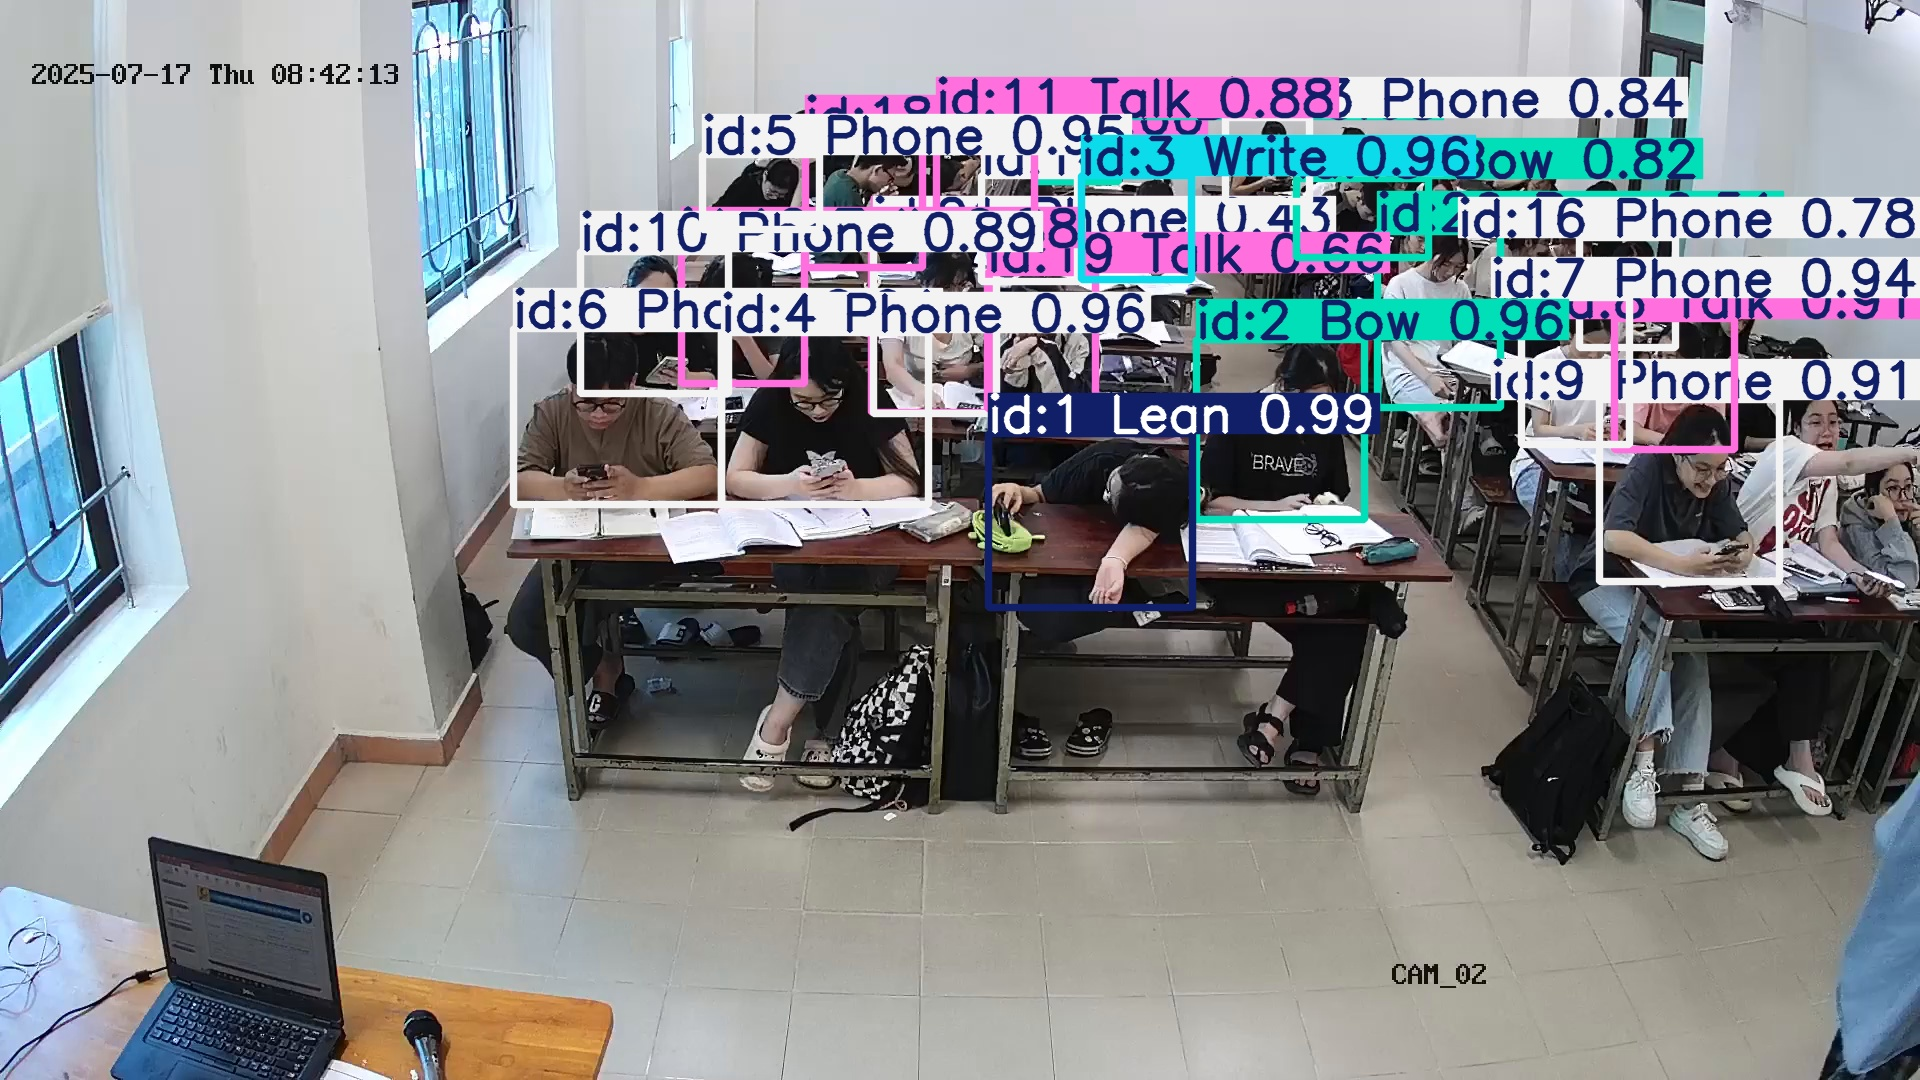
\includegraphics[width=0.7\textwidth]{figures/debug_frames/frame_00000000.jpg}
  \caption{Khung kiểm tra đại diện từ video thật tại frame 0.}
  \label{fig:case-study-debug-frame-0}
\end{figure}

\begin{figure}[htbp]
  \centering
  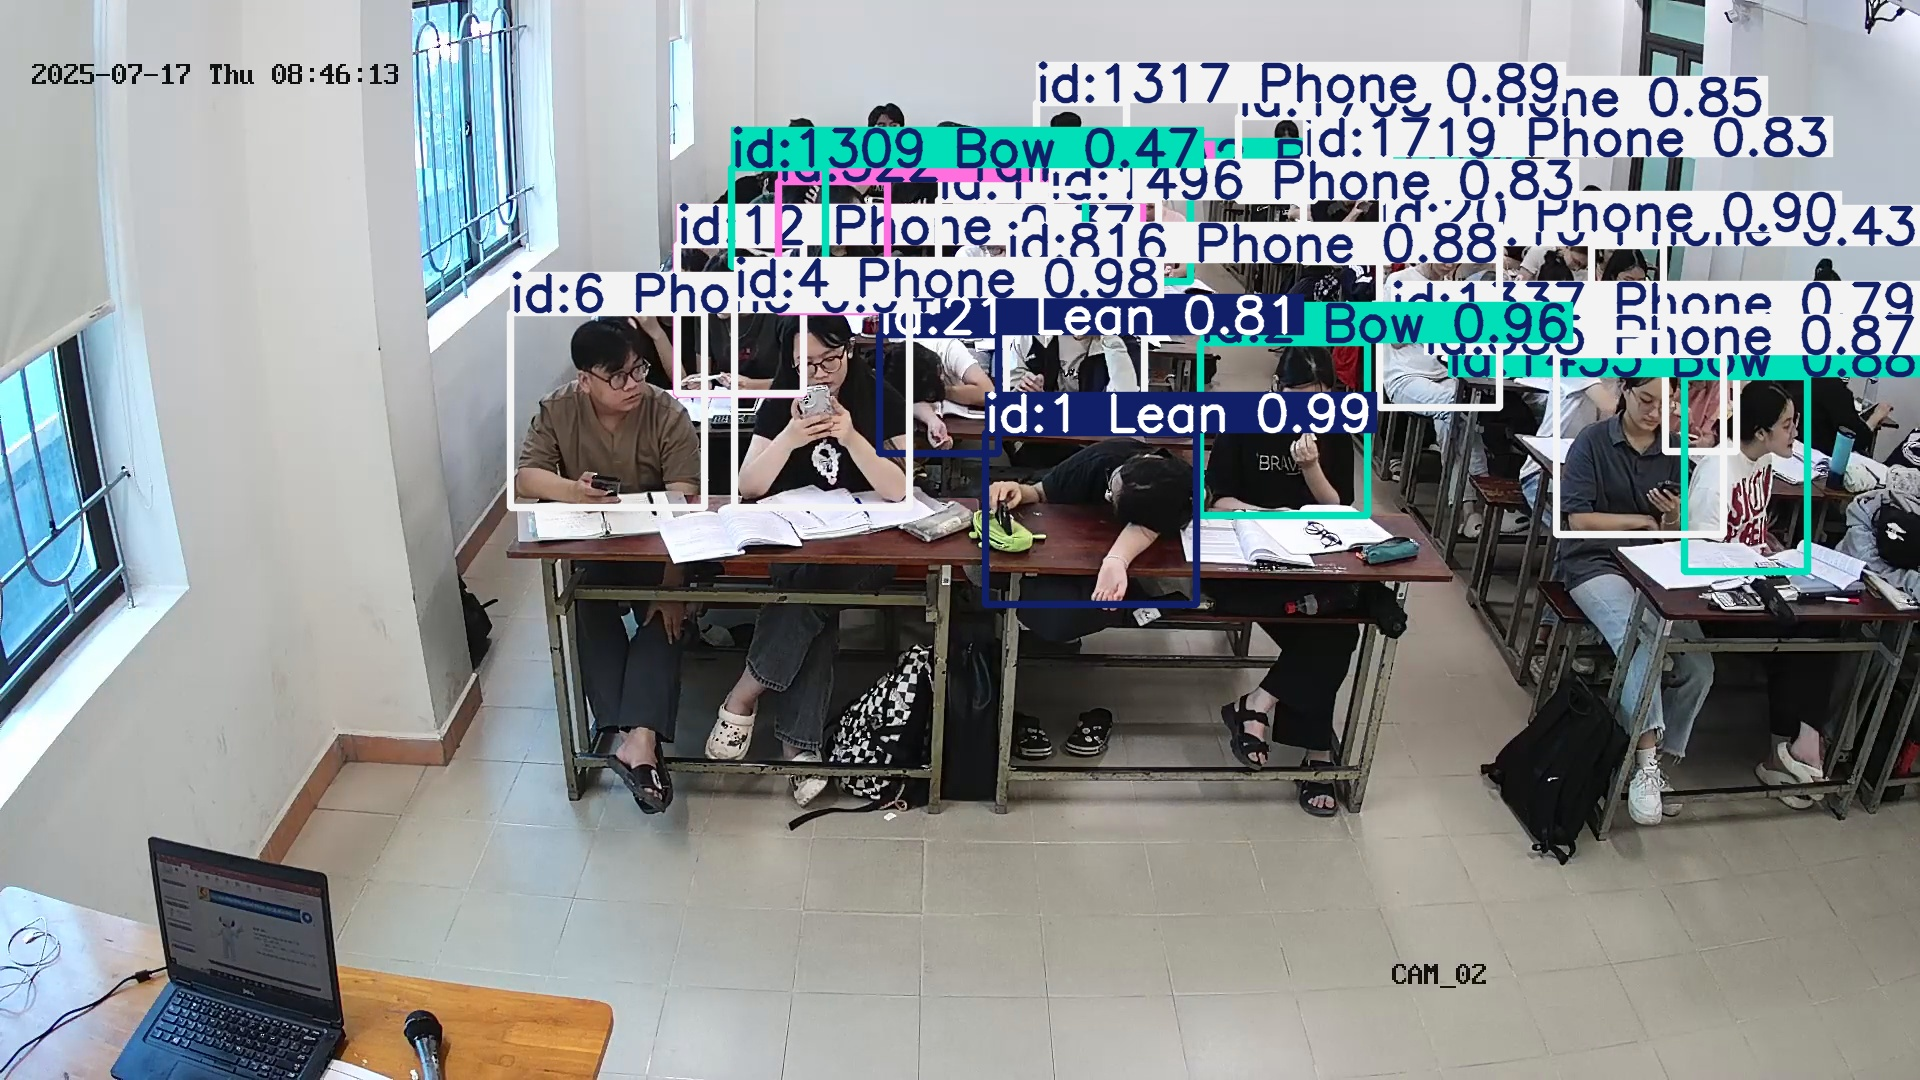
\includegraphics[width=0.7\textwidth]{figures/debug_frames/frame_00006000.jpg}
  \caption{Khung kiểm tra đại diện từ video thật tại frame 6000.}
  \label{fig:case-study-debug-frame-6000}
\end{figure}

\begin{figure}[htbp]
  \centering
  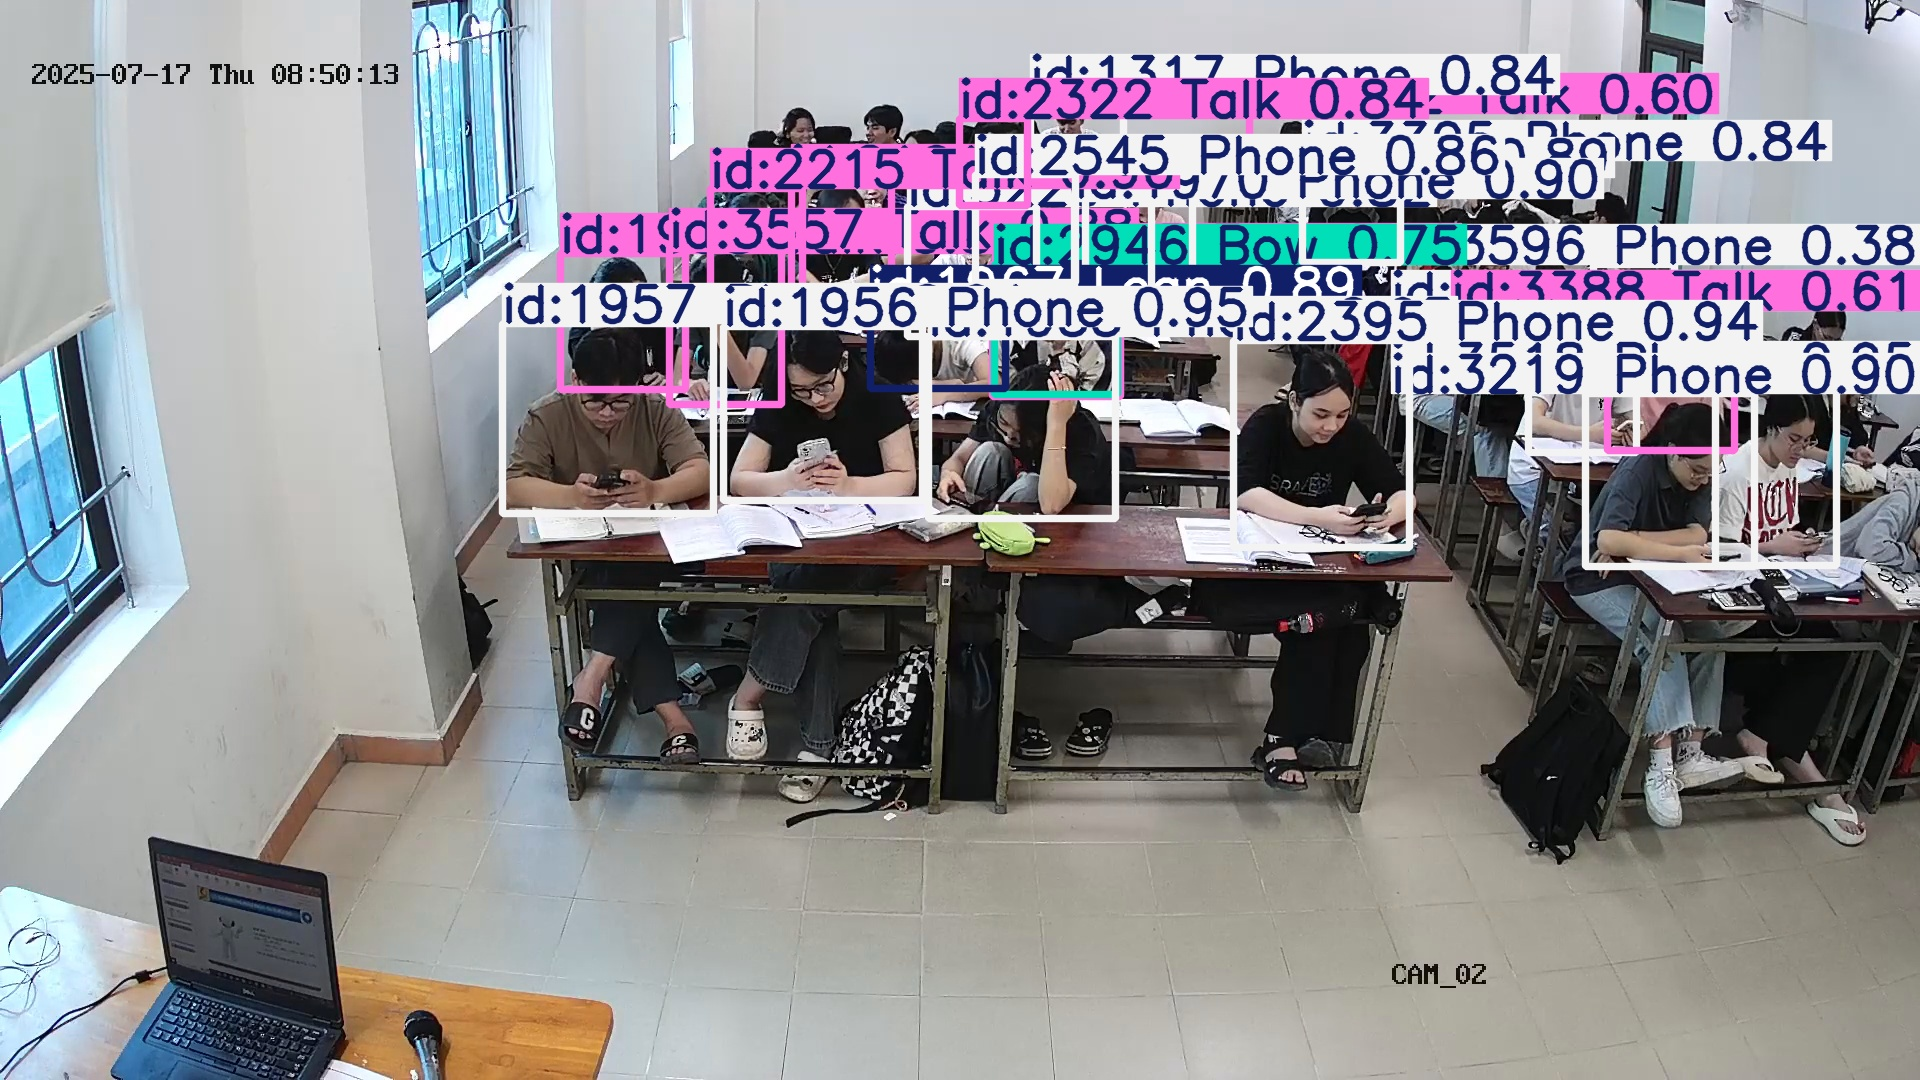
\includegraphics[width=0.7\textwidth]{figures/debug_frames/frame_00012000.jpg}
  \caption{Khung kiểm tra đại diện từ video thật tại frame 12000.}
  \label{fig:case-study-debug-frame-12000}
\end{figure}

\begin{table}[htbp]
\centering
\caption{Các đầu ra chính của case study.}
\label{tab:case-study-outputs}
\resizebox{\linewidth}{!}{%
\begin{tabular}{ll}
\toprule
\textbf{Nhóm đầu ra} & \textbf{Nội dung} \\
\midrule
Phát hiện & Danh sách sự kiện hành vi vi mô và khung kiểm tra \\
Chuỗi thời gian & CSV tỉ lệ hành vi theo 276 bin và siêu dữ liệu video \\
Đồ thị & Danh sách cạnh, ma trận kề, hình đồ thị và biểu đồ chuỗi thời gian \\
Báo cáo & Tóm tắt theo nguyên tắc nêu bằng chứng trước, dựa trên thống kê và cạnh đã kiểm chứng \\
\bottomrule
\end{tabular}
}
\end{table}

Đối với video thật, hệ thống sử dụng cùng logic beam search nhưng không tính Precision, Recall và F1 vì không có đồ thị chuẩn. Hệ số phạt cạnh kiểu BIC được đặt xấp xỉ \(\lambda=22\), được tỉ lệ hóa từ \(\lambda_{syn}=65\) của thực nghiệm tổng hợp theo độ dài chuỗi:
\begin{equation}
\label{eq:real-lambda-scaling}
    \lambda_{real}=\lambda_{syn}\frac{n_{real}}{n_{syn}}\frac{\log n_{syn}}{\log n_{real}}.
\end{equation}
Với \(n_{syn}=1000\) và \(n_{real}=276\), công thức cho giá trị xấp xỉ 22.06; quy trình dùng \(\lambda=22\) như một thiết lập thăm dò cho chuỗi thật ngắn hơn.

Trước khi sinh báo cáo, CausClass tạo hai nhóm bằng chứng đầu vào: thống kê mô tả của từng hành vi và các xu hướng biến đổi theo thời gian. Bảng~\ref{tab:case-study-descriptive-stats} tóm tắt nhóm bằng chứng thứ nhất. Các giá trị là phần trăm sự kiện hành vi được bộ phát hiện ghi nhận trong từng time bin, không phải phần trăm chính xác của toàn bộ học sinh trong lớp.

\begin{table}[htbp]
\centering
\caption{Thống kê mô tả hành vi trong case study.}
\label{tab:case-study-descriptive-stats}
\begin{tabular}{lrrrr}
\toprule
\textbf{Hành vi} & \textbf{Tỉ lệ TB} & \textbf{Cực đại} & \textbf{Độ lệch chuẩn} & \textbf{Tỉ lệ bin hoạt động} \\
\midrule
Phone & 40.624\% & 65.62\% & 13.444\% & 100.000\% \\
Talk & 28.345\% & 52.05\% & 9.967\% & 100.000\% \\
Bow & 18.789\% & 41.07\% & 8.772\% & 99.638\% \\
Read & 5.872\% & 37.33\% & 10.183\% & 29.348\% \\
Write & 3.843\% & 32.14\% & 6.886\% & 39.493\% \\
Lean & 2.527\% & 14.29\% & 2.786\% & 65.580\% \\
\bottomrule
\end{tabular}
\end{table}

Nhóm bằng chứng thứ hai là xu hướng theo thời gian. \textit{Phone} giảm dần với hệ số tuyến tính khoảng \(-0.100\) điểm phần trăm mỗi bin, trong khi \textit{Read} và \textit{Write} tăng lần lượt khoảng 0.091 và 0.049 điểm phần trăm mỗi bin. \textit{Bow} tăng nhẹ khoảng 0.020 điểm phần trăm mỗi bin, còn \textit{Lean} và \textit{Talk} giảm lần lượt khoảng \(-0.024\) và \(-0.036\) điểm phần trăm mỗi bin. Nếu chia video thành ba phần bằng nhau, \textit{Phone} vẫn là hành vi trội nhất ở cả ba phần, với trung bình 45.903\%, 46.863\% và 29.105\%. Ở phần cuối, \textit{Read} tăng lên 17.292\% và \textit{Write} tăng lên 10.096\%, trong khi \textit{Talk} giảm từ 36.838\% ở phần giữa xuống 20.987\%. Những lát cắt này chỉ là chia đoạn kỹ thuật của video, không nhất thiết tương ứng với các pha sư phạm của tiết học.

Từ các thống kê mô tả, xu hướng thời gian và danh sách cạnh đã kiểm chứng, hệ thống sinh báo cáo quan sát theo nguyên tắc nêu bằng chứng trước. Trong thiết lập triển khai, mô hình báo cáo là \textit{DeepSeek-v4-Pro}; mô hình nhận tóm tắt chuỗi thời gian và danh sách cạnh, sau đó trả về báo cáo JSON. Bộ kết xuất xác định chỉ trình bày lại các thông tin đã có trong đầu vào, nhờ đó tránh việc mô hình ngôn ngữ đổi tên cạnh, thêm cạnh mới hoặc diễn giải vượt quá bằng chứng.

Phần dưới đây là báo cáo quan sát được đưa vào case study. Báo cáo được biên tập theo hướng gọn hơn bản sinh ban đầu: các mục trùng nhau về diễn biến hành vi được gộp lại, các số liệu đã có trong bảng không bị lặp nguyên văn, còn các nhận xét quan trọng nhất được giữ để người quan sát biết nên kiểm tra đoạn video nào.

\subsection{Báo cáo quan sát}

\paragraph{Diễn biến chính.}
\textit{Phone} là hành vi chiếm ưu thế trong phiên quan sát, với tỉ lệ trung bình 40,6\% và cực đại 65,6\%, nhưng xu hướng chung giảm dần theo thời gian. \textit{Talk} và \textit{Bow} xuất hiện ổn định trong hầu hết các khoảng thời gian; \textit{Talk} đạt mức cao nhất ở giai đoạn giữa rồi giảm, còn \textit{Bow} tăng nhẹ. \textit{Read} và \textit{Write} nhìn chung ít xuất hiện hơn nhưng tăng rõ rệt trong một phần ba cuối phiên. \textit{Lean} là hành vi tương đối hiếm và có xu hướng giảm nhẹ.

\paragraph{Liên kết thời gian được phát hiện.}
Đồ thị cuối cùng gồm ba cạnh: \textit{Talk}\(\rightarrow\)\textit{Phone}, \textit{Talk}\(\rightarrow\)\textit{Read} và \textit{Phone}\(\rightarrow\)\textit{Read}. Trong đó, \textit{Talk}\(\rightarrow\)\textit{Phone} là liên kết dương mạnh nhất; \textit{Talk}\(\rightarrow\)\textit{Read} là liên kết dương yếu; còn \textit{Phone}\(\rightarrow\)\textit{Read} là liên kết âm yếu, gợi ý khả năng tồn tại sự đánh đổi giữa hai tín hiệu hành vi trong chuỗi quan sát.

\paragraph{Diễn giải có điều kiện.}
Mức \textit{Phone} cao có thể đi kèm với mức \textit{Read} thấp hơn ở thời điểm sau, nhưng nhận xét này chỉ là giả thuyết dựa trên liên kết thời gian. Liên kết giữa \textit{Talk} và \textit{Read} có thể xuất hiện trong các hoạt động hợp tác hoặc đọc thành tiếng, trong khi liên kết \textit{Talk}\(\rightarrow\)\textit{Phone} có thể phản ánh tương tác xã hội liên quan đến việc sử dụng điện thoại. Các cách diễn giải này cần được kiểm tra bằng video gốc, vì mô hình không quan sát được mục tiêu bài học, chỉ dẫn của giáo viên hoặc bối cảnh ngoài khung hình.

\paragraph{Điểm cần kiểm tra thủ công.}
Người quan sát nên xem lại các thời điểm \textit{Read} tăng mạnh để bảo đảm chúng không bị nhầm với tư thế \textit{Bow}; kiểm tra các bin mà \textit{Phone} đạt đỉnh để loại trừ khả năng phát hiện sai; xem lại các khoảng thời gian \textit{Write} gần như biến mất; và đối chiếu đoạn cuối phiên, nơi \textit{Read} và \textit{Write} tăng đột ngột. Những bước kiểm tra này giúp biến báo cáo tự động thành danh sách gợi ý kiểm chứng, thay vì kết luận sư phạm cuối cùng.

\subsection{Giao diện web phân tích trực quan}

Bên cạnh các tệp kết quả dạng bảng, đồ thị và báo cáo văn bản, case study còn được trình bày qua một giao diện web nhằm hỗ trợ quan sát trực quan toàn bộ quy trình phân tích. Giao diện này không thay đổi thuật toán phát hiện hay tìm kiếm đồ thị, mà đóng vai trò lớp tổng hợp kết quả để người dùng kiểm tra nhanh video đầu vào, thông số phân tích, thống kê mô tả, đồ thị liên kết thời gian, báo cáo quan sát và diễn biến các hành vi theo thời gian trong cùng một màn hình.

Hình~\ref{fig:web-visual-analysis-demo} minh họa bản demo của giao diện với video lớp học thật đã dùng trong case study. Phần đầu trang hiển thị thông tin video và số lượng time bin; cột trái tóm tắt thống kê mô tả và đồ thị thời gian; vùng giữa trình bày báo cáo quan sát theo các câu hỏi chính; còn cột phải trực quan hóa chuỗi thời gian của các hành vi. Cách bố trí này giúp người quan sát chuyển từ số liệu tổng hợp sang kiểm tra xu hướng cụ thể mà không phải mở riêng từng tệp đầu ra.

\begin{figure}[htbp]
  \centering
  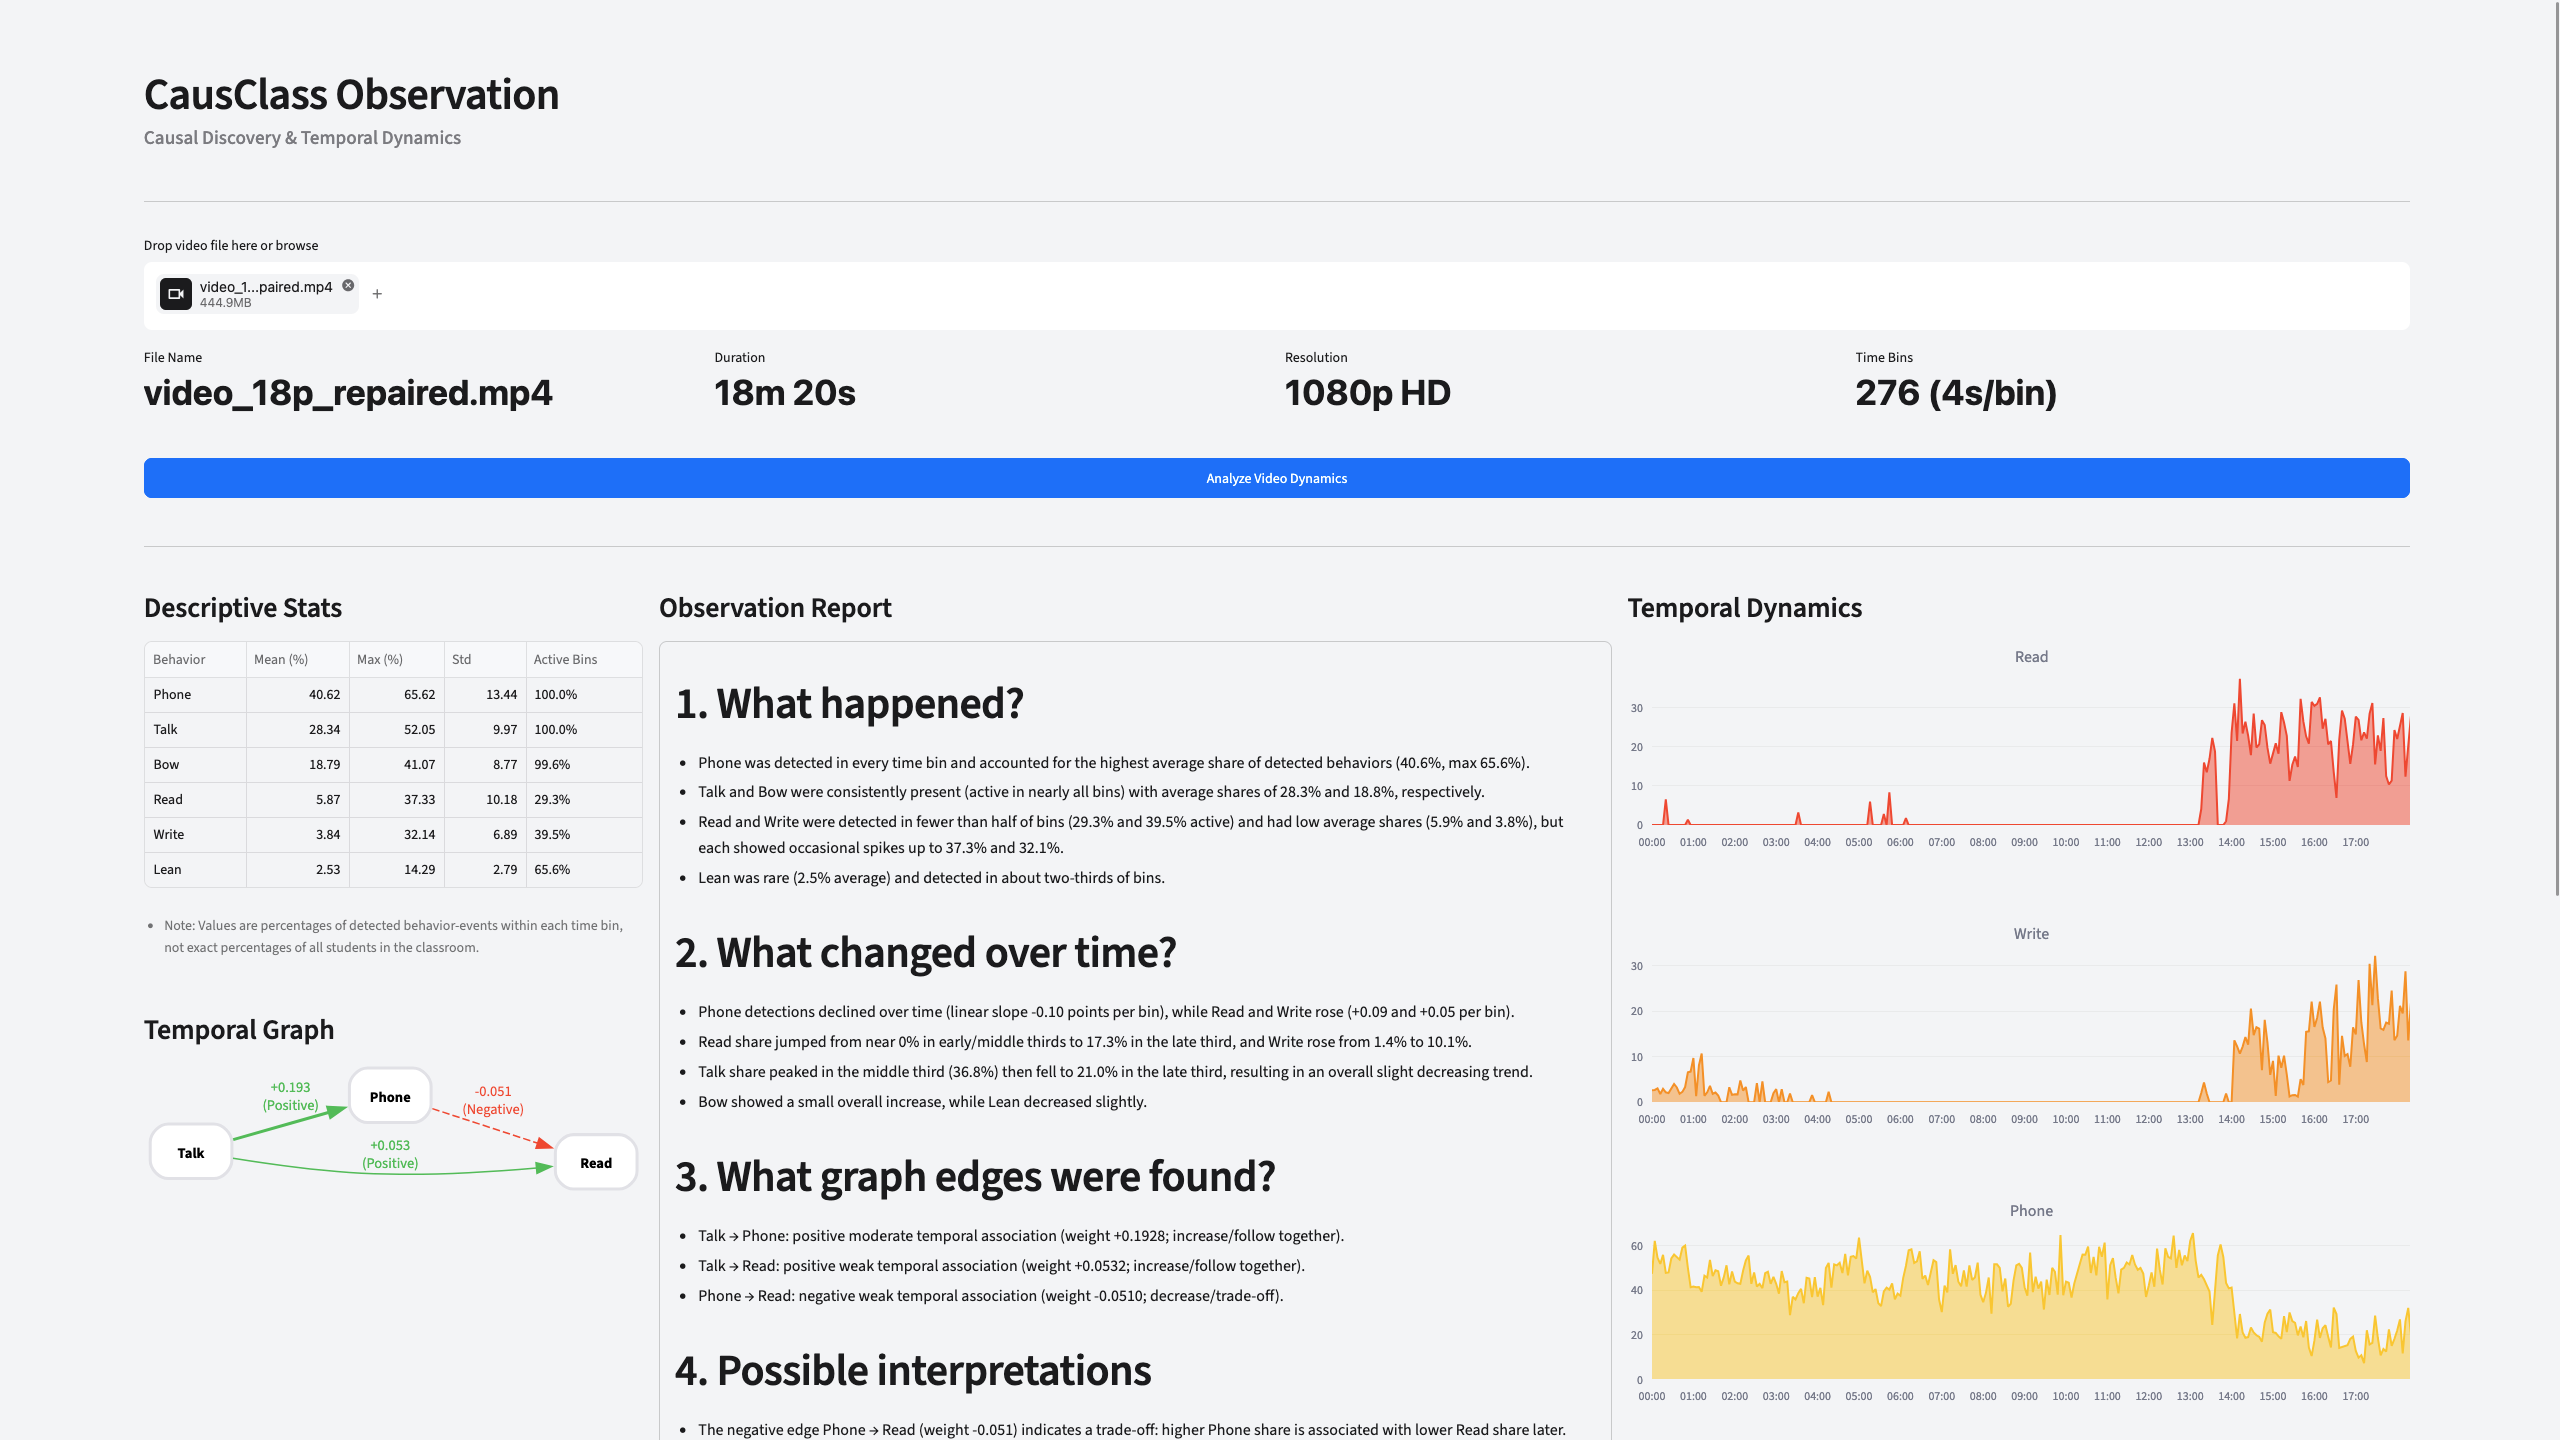
\includegraphics[width=\linewidth]{figures/web_visual_analysis_demo.png}
  \caption{Giao diện web demo dùng để phân tích trực quan kết quả case study CausClass.}
  \label{fig:web-visual-analysis-demo}
\end{figure}

Do giao diện chỉ hiển thị lại các kết quả đã được sinh từ pipeline, các biểu đồ và nhận xét trong màn hình vẫn cần được đọc theo cùng nguyên tắc thận trọng như báo cáo văn bản: chúng là bằng chứng quan sát được từ bộ phát hiện và chuỗi thời gian, không phải kết luận trực tiếp về nguyên nhân sư phạm. Tuy vậy, việc đặt bảng thống kê, đồ thị và báo cáo cạnh nhau giúp rút ngắn bước kiểm chứng thủ công, đặc biệt khi cần tìm nhanh các đoạn video có biến động mạnh hoặc các cạnh thời gian cần xem lại.

Tóm lại, case study cho thấy quy trình có thể vận hành từ video đầu vào đến báo cáo cuối cùng, đồng thời có thể được đóng gói thành giao diện trực quan để hỗ trợ kiểm tra kết quả. Nó cũng nhấn mạnh giới hạn của hệ thống: tỉ lệ phát hiện không phải tỉ lệ học sinh, các đoạn bằng nhau của video không nhất thiết là pha bài học, trọng số cạnh không phải kiểm định thống kê, và đồ thị không phải phán quyết về hành vi học sinh.

\newpage
\chapter{KẾT LUẬN}

\section{Kết luận}
Đồ án đã trình bày CausClass, một khung thống nhất cho phân tích hành vi lớp học từ video, tích hợp nhận diện hành vi tăng cường attention, khám phá liên kết thời gian và tinh chỉnh đồ thị có hướng dẫn bởi LLM. Hệ thống kết hợp YOLO26n-MHSA cho perception thị giác, AERCA cho mô hình hóa phụ thuộc thời gian, tìm kiếm beam có hướng dẫn bởi LLM cho tối ưu đồ thị, và báo cáo evidence-first để chuyển kết quả thành văn bản quan sát có thể kiểm tra.

Kết quả thực nghiệm cho thấy YOLO26n-MHSA cải thiện ổn định hiệu năng phát hiện so với YOLO26n trên các nhãn hành vi lớp học chung. Trên trung bình hai bộ dữ liệu, Recall tăng 0.0638, mAP@50 tăng 0.0250 và mAP@50--95 tăng 0.0266, trong khi Precision giảm nhẹ. Kết quả này ủng hộ vai trò của attention trong môi trường lớp học phức tạp, nơi hành vi thường phụ thuộc vào quan hệ không gian giữa đầu, tay, bàn học và vật thể nhỏ.

Đối với khám phá đồ thị thời gian, LLM-guided beam search đạt F1 cao nhất trên 100 bộ kiểm thử tổng hợp có ground truth, vượt các baseline AERCA trực tiếp, AERCA làm thưa, Random Beam và LLM Greedy. Điều này cho thấy tri thức ngữ nghĩa từ LLM có thể bổ sung hữu ích cho khám phá dữ liệu khi nó bị ràng buộc bởi verifier định lượng. LLM giúp đề xuất chỉnh sửa cấu trúc hợp lý hơn ngẫu nhiên, còn masked AERCA kiểm tra liệu chỉnh sửa đó có duy trì hoặc cải thiện dự báo dưới phạt độ phức tạp hay không.

Case study video lớp học thật minh họa tính khả thi của pipeline end-to-end: từ video đầu vào, hệ thống sinh khung debug, sự kiện vi mô, chuỗi thời gian hành vi, đồ thị liên kết thời gian và báo cáo quan sát. Tuy nhiên, case study không được dùng để khẳng định nhân quả. Các tỉ lệ hành vi là tỉ lệ sự kiện được detector ghi nhận, các phần ba video không phải pha bài học, trọng số cạnh là hệ số tương đối có dấu, và cạnh đồ thị không phải bằng chứng đạo đức hay kết luận sư phạm.

Đóng góp cốt lõi của đồ án vì vậy không nằm ở việc để một mô-đun tự động đưa ra phán quyết, mà ở cách ghép các mô-đun theo nguyên tắc kiểm chứng và truy vết. Detector tạo bằng chứng quan sát; chuỗi thời gian giữ cấu trúc thời gian; AERCA kiểm chứng đồ thị ứng viên; LLM chỉ đề xuất và hỗ trợ diễn giải có ràng buộc; báo cáo cuối cùng nhắc người dùng kiểm tra lại video. Cách thiết kế này hướng tới một hệ thống phân tích lớp học minh bạch, có kiểm chứng và thận trọng với giới hạn của dữ liệu quan sát.


\section{Giới hạn}
Mặc dù kết quả khả quan, đồ án vẫn có một số giới hạn quan trọng. Thứ nhất, đánh giá trên video lớp học thật còn hạn chế về quy mô, trong khi phần kiểm chứng định lượng đồ thị chủ yếu dựa trên benchmark tổng hợp do thiếu ground truth nhân quả hoặc ground truth liên kết thời gian do chuyên gia gán nhãn. Điều này có nghĩa là F1 đồ thị phản ánh khả năng khôi phục cấu trúc trong điều kiện mô phỏng có kiểm soát, chưa đủ để khẳng định độ chính xác cấu trúc trên mọi lớp học thật.

Thứ hai, quá trình xây dựng đồ thị nhạy với sai số của detector, độ thưa của quan sát và lựa chọn độ dài time bin. Chuỗi thời gian đầu vào của Stage 2 không phải quan sát trực tiếp của hành vi thật, mà là quan sát qua detector và tracker. Có thể mô tả đơn giản như
\begin{equation}
\label{eq:detector-noise-model}
    \widetilde{X}=X^{true}+\eta_{det},
\end{equation}
trong đó \(\eta_{det}\) là nhiễu do bỏ sót, phát hiện sai, phát hiện trùng, che khuất và góc quay. Nếu nhiễu này có cấu trúc theo thời gian, đồ thị học từ \(\widetilde{X}\) có thể khác đồ thị học từ \(X^{true}\).

Thứ ba, dữ liệu phát hiện trong đồ án có không gian nhãn khác nhau giữa Local và SCB, nên nghiên cứu cắt lớp chính chỉ báo cáo trên năm nhãn chung. Tập Local cũng có số ảnh huấn luyện tương đối nhỏ, vì vậy kết quả detector nên được xem như đánh giá thăm dò cho biến thể kiến trúc YOLO26n-MHSA, không phải kết luận cuối cùng cho mọi điều kiện lớp học.

Thứ tư, mô hình tổng hợp VAR(1) và time bin 4 giây là xấp xỉ kỹ thuật để tạo chuỗi kiểm thử ổn định và có ground truth. Nó không hàm ý rằng hành vi lớp học thật chỉ phụ thuộc vào bin ngay trước đó hoặc quan hệ giữa hành vi luôn tuyến tính. Các yếu tố như hoạt động của giáo viên, âm thanh, nội dung bài học, vị trí camera và bối cảnh lớp học có thể ảnh hưởng đến hành vi nhưng chưa được đo trong pipeline hiện tại.

Thứ năm, LLM vẫn có thể mang thiên lệch prior dù đã tách vai trò sinh ground truth và vai trò tìm kiếm, ngẫu nhiên hóa ngữ cảnh, dùng tabu list và kiểm chứng bằng AERCA. Các đề xuất của LLM có thể làm giảm không gian tìm kiếm, nhưng cũng có thể bỏ qua quan hệ ít quen thuộc hoặc ưu tiên quan hệ nghe hợp lý. Vì vậy, mọi kết quả LLM-guided phải được hiểu là kết quả của một quá trình đề xuất--kiểm chứng, không phải bằng chứng độc lập từ tri thức ngôn ngữ.

Cuối cùng, các quan hệ được phát hiện nên được diễn giải là liên kết thời gian được dữ liệu quan sát hỗ trợ, không phải hiệu ứng nhân quả dứt khoát. Điểm BIC-style là công cụ chọn mô hình, không phải kiểm định ý nghĩa thống kê đầy đủ; trọng số cạnh là hệ số tương đối của mô hình, không phải mức tác động sư phạm; và báo cáo tự động chỉ nên được dùng như hướng dẫn kiểm tra video, không phải kết luận thay con người.

\section{Hướng phát triển trong tương lai}
Hướng phát triển đầu tiên là mở rộng đánh giá trên các bộ dữ liệu lớp học lớn hơn, đa dạng hơn về trường học, môn học, vị trí camera, mật độ học sinh và điều kiện che khuất. Đối với Stage 1, cần thu thập thêm dữ liệu có nhãn thống nhất, chuẩn hóa không gian nhãn giữa các bộ dữ liệu và đánh giá thêm các biến thể attention để xác định vị trí chèn mô-đun tối ưu hơn. Việc có nhiều video thật hơn cũng cho phép kiểm tra độ ổn định của detector qua bối cảnh lớp học khác nhau.

Đối với Stage 2, hướng tiếp theo là xây dựng hoặc thu thập ground truth liên kết thời gian do chuyên gia gán nhãn, thay vì chỉ dựa vào dữ liệu tổng hợp. Đồng thời, cần so sánh trực tiếp với các baseline mạnh hơn như PCMCI, PCMCI+ và DYNOTEARS trên cùng bộ dữ liệu, đánh giá độ nhạy với hệ số phạt cạnh, số epoch fine-tune, beam width và chiến lược chia train/validation. Những thí nghiệm này sẽ giúp tách rõ lợi ích của bộ sinh đề xuất LLM, masked AERCA và beam search.

Một hướng kỹ thuật quan trọng là đánh giá bất định và độ ổn định của cạnh. Có thể chạy pipeline với nhiều độ dài bin \(\Delta t\), nhiều bootstrap hoặc nhiều lần suy luận detector, rồi đo độ ổn định của một cạnh bằng
\begin{equation}
\label{eq:edge-stability}
    \mathrm{Stability}(e)=\frac{1}{M}\sum_{m=1}^{M}\mathbf{1}\{e\in E_m\},
\end{equation}
trong đó \(E_m\) là đồ thị học được ở cấu hình hoặc mẫu bootstrap thứ \(m\). Các cạnh có stability cao sẽ đáng tin cậy hơn trong báo cáo quan sát, còn các cạnh chỉ xuất hiện ở một cấu hình nên được trình bày với cảnh báo mạnh hơn.

Một hướng mở rộng khác là xử lý tốt hơn quan sát thiếu và che khuất. Detector có thể bỏ sót hành vi khi học sinh bị che, vật thể nhỏ bị khuất hoặc camera không nhìn rõ bàn học. Các mô hình uncertainty-aware hoặc missing-data-aware có thể giúp Stage 2 phân biệt giữa ``không có hành vi'' và ``không quan sát được hành vi''. Điều này đặc biệt quan trọng với lớp học thật, nơi dữ liệu video hiếm khi sạch như dữ liệu mô phỏng.

Về báo cáo quan sát, có thể phát triển giao diện cho phép người dùng nhảy trực tiếp từ một thống kê hoặc một cạnh đồ thị tới các đoạn video liên quan. Giáo viên hoặc nhà nghiên cứu cũng có thể phản hồi rằng một cạnh là hợp lý, không rõ hoặc không hợp lý sau khi xem video. Phản hồi này không biến hệ thống thành công cụ phán xét tự động, mà giúp hiệu chỉnh detector, bộ gom sự kiện, bộ tìm kiếm đồ thị và ngôn ngữ báo cáo theo nhu cầu quan sát thực tế.

Cuối cùng, CausClass có thể được mở rộng sang dữ liệu giáo dục đa phương thức. Âm thanh lớp học, transcript, slide bài giảng, hoạt động của giáo viên và metadata của tiết học có thể cung cấp bối cảnh quan trọng mà video đơn lẻ không đo được. Kết hợp các nguồn này có thể giúp hệ thống phân biệt tốt hơn giữa hành vi giống nhau về hình ảnh nhưng khác ý nghĩa sư phạm, đồng thời cải thiện độ tin cậy của các nhận xét được sinh ra từ pipeline.

\newpage
\renewcommand\bibname{TÀI LIỆU THAM KHẢO}
\printbibliography
\phantomsection\addcontentsline{toc}{chapter}{TÀI LIỆU THAM KHẢO}

\appendixpage
\appendix
\addappheadtotoc

\titleformat{\chapter}
    [hang]
    {\centering\bfseries}
    {\thechapter.\ }
    {0pt}
    {}
    []
\titlespacing*{\chapter}{0pt}{-20pt}{20pt}

\titlecontents{chapter}
    [0.0cm]
    {\bfseries\vspace{0.3cm}}
    {{\bfseries{\scshape} \thecontentslabel.\ }}
    {}
    {\titlerule*[0.3pc]{.}\contentspage}

\chapter{FILE CẤU HÌNH YOLO26N-MHSA}
\label{appendix:yolo26n-mhsa-yaml}
Phụ lục này trình bày cấu hình kiến trúc YOLO26n-MHSA được sử dụng trong Stage 1. Cấu hình giữ phần lớn backbone và head của YOLO26n, đồng thời chèn mô-đun MHSA tại layer 20 trước khi hợp nhất đặc trưng cho lớp phát hiện cuối.

\renewcommand{\lstlistingname}{Đoạn mã}
\begin{lstlisting}[
caption={Cấu hình YAML của YOLO26n-MHSA.},
label={lst:yolo26n-mhsa-yaml},
basicstyle=\ttfamily\small,
breaklines=true,
columns=fullflexible,
keepspaces=true,
frame=single,
showstringspaces=false
]
topology_yaml = """
nc: 6 
scales:
  n: [0.50, 0.25, 1024]
backbone:
  - [-1, 1, Conv, [64, 3, 2]]           # 0
  - [-1, 1, Conv, [128, 3, 2]]          # 1
  - [-1, 2, C3k2, [256, False, 0.25]]   # 2
  - [-1, 1, Conv, [256, 3, 2]]          # 3
  - [-1, 2, C3k2, [512, False, 0.25]]   # 4  
  - [-1, 1, Conv, [512, 3, 2]]          # 5
  - [-1, 2, C3k2, [512, True]]          # 6  
  - [-1, 1, Conv, [1024, 3, 2]]         # 7
  - [-1, 2, C3k2, [1024, True]]         # 8
  - [-1, 1, SPPF, [1024, 5, 3, True]]   # 9
  - [-1, 2, C2PSA, [1024]]              # 10 

head:
  - [-1, 1, nn.Upsample, [None, 2, 'nearest']]
  - [[-1, 6], 1, Concat, [1]]           # 12
  - [-1, 2, C3k2, [512, True]]          # 13 
  - [-1, 1, nn.Upsample, [None, 2, 'nearest']]
  - [[-1, 4], 1, Concat, [1]]           # 15
  - [-1, 2, C3k2, [256, True]]          # 16 
  
  - [-1, 1, Conv, [256, 3, 2]]          # 17
  - [[-1, 13], 1, Concat, [1]]          # 18
  - [-1, 2, C3k2, [512, True]]          # 19
  
  - [-1, 1, MHSA, [128, 128]]           # 20 
  
  - [-1, 1, Conv, [512, 3, 2]]          # 21
  - [[-1, 10], 1, Concat, [1]]          # 22
  - [-1, 1, C3k2, [1024, True, 0.5, True]] # 23
  
  - [[16, 20, 23], 1, Detect, [nc]]     # 24
"""
\end{lstlisting}

\chapter{CÁC PROMPT SỬ DỤNG TRONG HỆ THỐNG}
\label{appendix:prompts}
Phụ lục này trình bày các prompt được sử dụng trong hệ thống, bao gồm prompt sinh test, prompt đề xuất chỉnh sửa đồ thị và prompt sinh báo cáo quan sát.

\section{Prompt sinh test}

Prompt sinh test được dùng để yêu cầu mô hình ngôn ngữ tạo đồ thị nhân quả vĩ mô của lớp học dưới dạng DAG cho mô hình chuỗi thời gian VAR(1). Đầu ra mong muốn là một đối tượng JSON có khóa \texttt{edges}; mỗi cạnh gồm nguồn, đích, dấu tác động, độ mạnh và giải thích.

\begin{lstlisting}[
caption={Prompt sinh test đồ thị nhân quả vĩ mô trong lớp học.},
label={lst:test-generation-prompt},
basicstyle=\ttfamily\small,
breaklines=true,
columns=fullflexible,
keepspaces=true,
frame=single,
showstringspaces=false
]
prompt = f"""You are an Expert Data Scientist modeling a MACROSCOPIC classroom causal graph (DAG) for a Time-Series VAR(1) model.
Context: {context}

AVAILABLE BEHAVIORS:
- 'Talk': Widespread student-to-student chatting (Creates a noisy environment).
- 'Read': A high percentage of the class focusing on reading textbooks.
- 'Phone': Epidemic of covert smartphone usage.
- 'Hand': Multiple students raising hands to ask questions.
- 'Lean': Widespread slouching or leaning on desks.
- 'Stand': Groups of students standing up.

CRITICAL RULES FOR ALIGNMENT (YOUR GRAPH WILL BE REVIEWED BY A RUTHLESS PRUNER):
1. BEHAVIORS MUST PHYSICALLY CAUSE BEHAVIORS. Do not invent butterfly-effect causality.
   - ACCEPTABLE: "Widespread talking creates noise, reducing the percentage of students reading." (Talk -> Read, negative)
   - ACCEPTABLE: "High phone usage isolates students, reducing peer-to-peer talking." (Phone -> Talk, negative)
2. THINK IN PEER INFLUENCE & CONTAGION, NOT INDIVIDUAL SEQUENCES.
3. Output MUST be a STRICT Directed Acyclic Graph (DAG). NO feedback loops.
4. Output format: JSON object with a single key "edges" containing a list of edges.
Each edge MUST have: "source", "target", "type" ('positive' or 'negative'), "strength" ('medium', 'high' ONLY), and "reasoning".

Generate EXACTLY {min_edges} to {max_edges} bulletproof, highly logical MACRO-LEVEL causal edges that represent DIRECT PHYSICAL/ENVIRONMENTAL INFLUENCE.
"""
\end{lstlisting}

\section{Các biến đầu vào của prompt sinh test}

Ba biến được chèn vào prompt bằng cơ chế f-string của Python:
\begin{itemize}
\item \texttt{context}: mô tả ngữ cảnh lớp học cho từng lần sinh test. Biến này giúp mỗi đồ thị được tạo gắn với một tình huống cụ thể, ví dụ thời điểm trong ngày, dạng bài học và sự kiện đang diễn ra trong lớp.
\item \texttt{min\_edges}: số cạnh tối thiểu mà mô hình cần sinh. Tham số này kiểm soát cận dưới về độ dày của đồ thị kiểm thử.
\item \texttt{max\_edges}: số cạnh tối đa mà mô hình được phép sinh. Tham số này kiểm soát cận trên về độ dày của đồ thị, tránh việc mô hình thêm quá nhiều liên kết khó kiểm chứng.
\end{itemize}

Trong triển khai, biến \texttt{context} được sinh động bằng cách lấy ngẫu nhiên một thời điểm, một loại bài học và một sự kiện lớp học:

\begin{lstlisting}[
caption={Hàm sinh ngữ cảnh động cho prompt sinh test.},
label={lst:dynamic-context-generator},
basicstyle=\ttfamily\small,
breaklines=true,
columns=fullflexible,
keepspaces=true,
frame=single,
showstringspaces=false
]
def generate_dynamic_context():
    times = ["early morning", "mid-morning", "post-lunch food coma", "late afternoon"]
    subjects = ["Calculus lecture", "boring History reading", "interactive discussion"]
    events = ["stressful exam coming up", "teacher is strict", "teacher has back turned"]
    return f"Time: {random.choice(times)}. Subject: {random.choice(subjects)}. Event: {random.choice(events)}."
\end{lstlisting}

Do đó, mỗi lời gọi hàm có thể tạo một ngữ cảnh khác nhau, chẳng hạn lớp học buổi sáng sớm, tiết đọc lịch sử nhàm chán hoặc tình huống giáo viên quay lưng. Ngữ cảnh này không trực tiếp quyết định cạnh nào phải xuất hiện, nhưng định hướng mô hình chọn các quan hệ phù hợp hơn với điều kiện quan sát.

\section{Prompt đề xuất chỉnh sửa đồ thị}

Prompt đề xuất chỉnh sửa đồ thị được dùng cho tác nhân \textit{Pruning Agent} trong CausClass. Nhiệm vụ của tác nhân là nhận đồ thị hiện tại từ quy trình tìm kiếm, xem các tín hiệu liên kết còn thiếu và đề xuất một số thao tác \texttt{add} hoặc \texttt{delete} để làm sạch đồ thị. Prompt được tách thành hai phần nhằm tối ưu hóa prompt cache: phần \texttt{system\_prompt} chứa các định nghĩa và luật cố định, còn phần \texttt{user\_prompt} chứa trạng thái động của từng bước tìm kiếm.

Các quy tắc trong system prompt được hình thành từ hai nguồn. Một phần đến từ gợi ý của mô hình ngôn ngữ về cách ràng buộc bài toán ở mức vĩ mô. Phần còn lại đến từ quá trình prompt engineering: quan sát các đầu ra sai hoặc yếu của mô hình, nhận diện các kiểu lỗi lặp lại, rồi thêm quy tắc để ngăn chặn. Vì vậy, một số quy tắc có thể trông không trực giác ngay từ đầu, nhưng được dùng để chặn các lỗi cụ thể như xóa cạnh chỉ vì quan hệ có dấu âm, quy mọi hành vi về trạng thái ẩn, hoặc thêm cạnh ngoài tập nút cho phép.

\subsection{System prompt cố định}

\begin{lstlisting}[
caption={System prompt cho tác nhân đề xuất chỉnh sửa đồ thị.},
label={lst:graph-edit-system-prompt},
basicstyle=\ttfamily\small,
breaklines=true,
columns=fullflexible,
keepspaces=true,
frame=single,
showstringspaces=false
]
system_prompt = f"""PROJECT CONTEXT: You are the core 'Pruning Agent' for "CausClass", a system designed to discover macro-level classroom behavior graphs from noisy Time-Series data. The baseline mathematical engine (AERCA) has extracted a messy graph full of spurious correlations. YOUR JOB IS TO CLEAN IT UP.

CRITICAL MACRO-LEVEL DEFINITIONS (MUST USE THESE):
- 'Talk': Widespread student-to-student chatting (Contagious noise).
- 'Read': A high percentage of the class focusing on reading.
- 'Phone': Epidemic of covert smartphone usage (Signals contagious isolation).
- 'Hand': Multiple students raising hands (High collective engagement).
- 'Lean': Widespread slouching/leaning (Contagious fatigue/low energy).
- 'Stand': Groups of students standing up.

CRITICAL CAUSALITY RULES (READ CAREFULLY BEFORE DELETING):
1. STRUCTURAL GRAPH ONLY: The edges provided to you represent STRUCTURAL CONNECTIONS ONLY. They DO NOT imply a positive or negative sign.
2. NEGATIVE CAUSALITY IS VALID: If A suppresses/decreases B (e.g., Talking suppresses Reading), the structural link EXISTS and is VALID. 
3. DO NOT BE THE SIGN POLICE: NEVER propose deleting an edge by arguing "it suppresses B, so the positive sign is wrong". If A impacts B in ANY WAY (increasing OR suppressing), YOU MUST KEEP THE EDGE. DO NOT DELETE IT!

CRITICAL PRUNING AND ADDING RULES:
1. BEHAVIORS CAUSE BEHAVIORS (NO LATENT STATES): You MUST assume that behaviors directly influence other behaviors through peer contagion or physical disruption. NEVER delete an edge by arguing that both behaviors are just "symptoms" of a hidden internal state (like 'boredom', 'engagement', 'fatigue', 'energy', or 'motivation'). 
2. NEGATIVE CAUSALITY = KEEP: If behavior A creates an environment that suppresses behavior B (e.g., Talking creates noise that stops Reading; Phone use isolates students and stops Talking), YOU MUST KEEP THE EDGE. 
3. DELETE ONLY ABSURD PHYSICAL SEQUENCES: Only delete an edge if the physical sequence is absurd (e.g., Reading causes Standing, or Standing causes Leaning). 
4. NO HALLUCINATIONS: Evaluate ONLY the nodes provided. Do not invent root causes.
5. THE 'ADD' ACTION (RESURRECTION): You will be provided with 'SUSPECTED MISSING LINKS' (strong mathematical signals ignored by the baseline). If one of these missing links makes PERFECT MACRO-LOGICAL SENSE (e.g., Talk suppresses Read, Phone suppresses Talk), output an 'add' action! Do not add blindly, only add if the behavior clearly drives or suppresses the target.

OUTPUT FORMAT: Return ONLY a valid JSON object containing an "edits" key mapped to an array of 1 to 3 objects.
EXAMPLE:
{{
  "edits": [
    {{"action": "delete", "source": "Read", "target": "Stand", "reasoning": "Reading is stationary, it does not physically cause standing."}},
    {{"action": "add", "source": "Talk", "target": "Read", "reasoning": "Widespread talking creates a disruptive noise environment that heavily suppresses reading."}}
  ]
}}

"""
\end{lstlisting}

\subsection{User prompt động}

\begin{lstlisting}[
caption={User prompt chứa trạng thái động của bước tối ưu đồ thị.},
label={lst:graph-edit-user-prompt},
basicstyle=\ttfamily\small,
breaklines=true,
columns=fullflexible,
keepspaces=true,
frame=single,
showstringspaces=false
]
user_prompt = f"""
=== CURRENT GRAPH TO OPTIMIZE ===
{self.format_current_graph(current_edges)}

=== SUSPECTED MISSING LINKS (MATH SIGNALS) ===
{hint_str}

TABU LIST (DO NOT SUGGEST THESE EDGES): {json.dumps(local_tabu)}
SYSTEM FEEDBACK (Prior MSE impacts): {feedback_momentum}

TASK: Return a JSON object with the "edits" array containing 1 to 3 strictly evaluated edits.
"""
\end{lstlisting}

\subsection{Các biến đầu vào của prompt chỉnh sửa đồ thị}

Các biến trong phần động phản ánh trạng thái hiện tại của vòng tìm kiếm:
\begin{itemize}
\item \texttt{current\_edges}: danh sách cạnh hiện có của đồ thị đang được tối ưu. Đây là đối tượng mà mô hình cần xem xét để đề xuất xóa cạnh không hợp lý hoặc giữ lại các liên kết có cơ sở vĩ mô.
\item Hàm \texttt{format\_current\_graph}: chuyển \texttt{current\_edges} thành chuỗi văn bản dễ đọc cho mô hình, thường gồm các cặp nguồn--đích đang có trong đồ thị.
\item \texttt{hint\_str}: chuỗi mô tả các liên kết nghi ngờ bị thiếu. Các liên kết này đến từ tín hiệu toán học nhưng chưa có trong đồ thị hiện tại, nên chỉ nên được thêm nếu có diễn giải hành vi vĩ mô hợp lý.
\item \texttt{local\_tabu}: danh sách cấm cục bộ trong bước tìm kiếm hiện tại. Các cạnh trong danh sách này không được đề xuất lại, nhằm tránh lặp vòng, tránh các chỉnh sửa vừa bị bác bỏ hoặc các cạnh đã biết là không nên thử.
\item Lời gọi \texttt{json.dumps}: tuần tự hóa danh sách \texttt{local\_tabu} thành chuỗi JSON để đưa vào prompt một cách rõ ràng và ít mơ hồ.
\item \texttt{feedback\_momentum}: tóm tắt phản hồi từ các lần thử trước, đặc biệt là tác động của các chỉnh sửa lên MSE. Biến này giúp mô hình ưu tiên các hướng chỉnh sửa từng cải thiện tiêu chí đánh giá và tránh các hướng từng làm kết quả xấu đi.
\end{itemize}

Nhờ cách tách này, phần định nghĩa hành vi và luật kiểm soát đầu ra có thể được tái sử dụng qua nhiều lượt gọi, trong khi chỉ phần trạng thái đồ thị, tín hiệu thiếu cạnh, danh sách tabu và phản hồi định lượng thay đổi theo từng vòng tối ưu.

\section{Prompt sinh báo cáo quan sát}

Prompt sinh báo cáo quan sát được dùng ở bước cuối của hệ thống để chuyển dữ liệu phát hiện hành vi và đồ thị đã kiểm chứng thành báo cáo ngắn gọn, nêu bằng chứng trước. Prompt này nhấn mạnh rằng hệ thống không có ngữ cảnh bài học, tỉ lệ hành vi là tỉ lệ sự kiện phát hiện theo bin thời gian, và các cạnh đồ thị chỉ là liên kết thời gian chứ không phải bằng chứng nhân quả.

\begin{lstlisting}[
caption={Prompt sinh báo cáo quan sát từ dữ liệu phát hiện hành vi.},
label={lst:observation-report-prompt},
basicstyle=\ttfamily\small,
breaklines=true,
columns=fullflexible,
keepspaces=true,
frame=single,
showstringspaces=false
]
You are a classroom observation analyst. Produce a compact evidence-first report from behavior-detection data.

Hard limits:
- No lesson context is available.
- Behavior shares are detected-event shares per time bin, not student percentages.
- Graph edges are temporal associations, not proof of causality.
- Respect the graph exactly. Do not ignore, rename, reverse, merge, or invent graph edges.
- Graph direction matters: A -> B means A at an earlier step is associated with B later. Do not infer B -> A unless that edge exists.
- Use every final graph edge when forming interpretations; if an edge is weak, explicitly call it weak instead of omitting it.
- Do not mention any time window, timestamp, or phase boundary unless it is explicitly present in time_series_summary.
- Do not claim an arbitrary early slice is a meaningful lesson phase.
- Do not judge students or claim off-task behavior.
- Do not recommend punishment, phone bans, phone stacks, phone parking, shaming, or policy changes.
- Keep teacher-facing wording simple; this report is for classroom review, not a research paper.
- Section 1 must not contain graph-derived claims; save all graph reasoning for possible_interpretations.
- No markdown. Return JSON only.

Return exactly one valid JSON object with these keys:
{
  "what_happened": [2 to 4 short bullets containing ONLY descriptive detection facts: frequent/rare behaviors, active bins, mean shares; DO NOT mention graph edges, causality, associations, trade-offs, or interpretations],
  "changed_over_time": [2 to 4 short bullets based ONLY on trend_by_behavior and temporal_segments; explicitly treat early/middle/late as equal video thirds, not lesson phases],
  "possible_interpretations": [2 to 3 bullets, each with evidence + alternate explanation; use the graph here, respect direction, and mention weak edges as weak],
  "human_inspection": [3 to 5 specific debug-frame checks],
}

Section rules:
- Section 1 / what_happened must be pure observation. Do not mention Phone -> Read, Talk -> Read, negative edge, positive edge, association, trade-off, or causal language there.
- Section 2 / changed_over_time may compare equal video thirds and trend directions, but must not imply those thirds are lesson phases.
- Section 3 will be rendered exactly by the program from the verified graph. Do NOT include a graph_edges_found key.
- Section 4 / possible_interpretations may interpret graph edges, but must not reverse edge direction. A -> B does not mean B -> A.
- Each bullet must be one sentence. Keep the whole report readable, but do not omit required sections just to be short.
\end{lstlisting}

Các trường đầu vào chính mà prompt dựa vào gồm \texttt{time\_series\_summary}, \texttt{trend\_by\_behavior}, \texttt{temporal\_segments} và đồ thị cuối cùng đã được kiểm chứng. Trong đó, \texttt{time\_series\_summary} cung cấp thống kê mô tả theo thời gian, \texttt{trend\_by\_behavior} mô tả xu hướng của từng hành vi, \texttt{temporal\_segments} mô tả các phần bằng nhau của video, còn đồ thị cuối cùng cung cấp các liên kết thời gian được phép dùng trong phần diễn giải.

\chapter{HƯỚNG DẪN CÀI ĐẶT MÔI TRƯỜNG VÀ CHẠY THỬ NGHIỆM}
\label{appendix:environment-setup}
\markboth{PHỤ LỤC C. HƯỚNG DẪN CÀI ĐẶT}{}

Phụ lục này trình bày hướng dẫn cài đặt môi trường, cấu hình khóa API và các lệnh chạy thử nghiệm chính của dự án CausClass. Nội dung chỉ tập trung vào các bước cần thiết để thiết lập và chạy các pipeline thực nghiệm.

\section{Yêu cầu môi trường}

Dự án nên được chạy với Python 3.11 nếu có thể. CausClass kết hợp YOLO và ByteTrack cho nhận diện và theo dõi hành vi. Hệ thống dùng Gemini 3 Flash cho sinh dữ liệu tổng hợp, DeepSeek cho đề xuất chỉnh sửa đồ thị và sinh báo cáo quan sát, đồng thời dùng AERCA như bộ kiểm chứng neural cho các đồ thị ứng viên.

Trong dự án này, AERCA chỉ được dùng như máy kiểm chứng bên trong CausClass. Nếu sử dụng mã nguồn hoặc kết quả có liên quan tới AERCA, cần trích dẫn bài báo gốc của AERCA.

\section{Cài đặt thư viện}

Các bước cài đặt cơ bản như sau:

\begin{lstlisting}[
caption={Cài đặt môi trường Python cho CausClass.},
label={lst:causclass-installation},
basicstyle=\ttfamily\small,
breaklines=true,
columns=fullflexible,
keepspaces=true,
frame=single,
showstringspaces=false
]
python3 -m venv .venv
source .venv/bin/activate
pip install --upgrade pip
pip install -r requirements.txt
\end{lstlisting}

Với các thử nghiệm cần CUDA cho huấn luyện hoặc suy luận, cần cài đặt phiên bản PyTorch phù hợp với CUDA driver của máy từ trình chọn cài đặt chính thức của PyTorch, sau đó cài đặt các phụ thuộc còn lại của dự án bằng \texttt{requirements.txt}.

\section{Cấu hình biến môi trường}

Tạo tệp \texttt{.env} ở thư mục gốc của dự án để lưu khóa API:

\begin{lstlisting}[
caption={Cấu hình khóa API trong tệp .env.},
label={lst:causclass-env},
basicstyle=\ttfamily\small,
breaklines=true,
columns=fullflexible,
keepspaces=true,
frame=single,
showstringspaces=false
]
GEMINI_API_KEY=your_gemini_key_here
DEEPSEEK_API_KEY=your_deepseek_key_here
\end{lstlisting}

\texttt{GEMINI\_API\_KEY} được dùng cho bước sinh dữ liệu tổng hợp. Theo mặc định, bộ sinh dữ liệu dùng Gemini 3 Flash với mã mô hình \texttt{gemini-3-flash-preview}. Nếu Google thay đổi tên mô hình được khuyến nghị, có thể ghi đè bằng biến \texttt{GEMINI\_SYNTHETIC\_MODEL}.

\texttt{DEEPSEEK\_API\_KEY} được dùng cho các đề xuất chỉnh sửa đồ thị và bước sinh báo cáo quan sát cuối cùng. Khi chỉ chạy thử cục bộ và không muốn ghi log lên Weights \& Biases, có thể đặt thêm biến sau:

\begin{lstlisting}[
caption={Tắt Weights \& Biases cho chạy thử cục bộ.},
label={lst:causclass-wandb-disabled},
basicstyle=\ttfamily\small,
breaklines=true,
columns=fullflexible,
keepspaces=true,
frame=single,
showstringspaces=false
]
WANDB_MODE=disabled
\end{lstlisting}

\section{Các lệnh sử dụng thường gặp}

\subsection{Chạy pipeline video đầu-cuối}

Lệnh sau chạy toàn bộ pipeline từ video lớp học tới các kết quả đầu ra, bao gồm phát hiện hành vi, xây dựng chuỗi thời gian, tìm kiếm đồ thị và lưu các artifact:

\begin{lstlisting}[
caption={Chạy pipeline đầu-cuối trên một video lớp học.},
label={lst:causclass-end-to-end},
basicstyle=\ttfamily\small,
breaklines=true,
columns=fullflexible,
keepspaces=true,
frame=single,
showstringspaces=false
]
python -m core.end_to_end_pipeline \
  --video data/videos/classroom.mp4 \
  --model data/best.pt \
  --output_dir output/runs/classroom_001
\end{lstlisting}

\subsection{Chỉ trích xuất động học hành vi từ video}

Nếu chỉ cần chạy pha nhận diện và trích xuất chuỗi thời gian hành vi từ video, sử dụng lệnh sau:

\begin{lstlisting}[
caption={Trích xuất động học hành vi từ video.},
label={lst:causclass-extract-video-dynamics},
basicstyle=\ttfamily\small,
breaklines=true,
columns=fullflexible,
keepspaces=true,
frame=single,
showstringspaces=false
]
python -m data.extract_video_dynamics data/videos/classroom.mp4 \
  --model data/best.pt \
  --output-dir output/phase1/classroom_001
\end{lstlisting}

\subsection{Chạy khám phá đồ thị trên tệp CSV có sẵn}

Khi đã có chuỗi thời gian hành vi ở dạng CSV, có thể chạy riêng bước khám phá đồ thị:

\begin{lstlisting}[
caption={Chạy khám phá đồ thị từ chuỗi thời gian hành vi có sẵn.},
label={lst:causclass-causal-discovery},
basicstyle=\ttfamily\small,
breaklines=true,
columns=fullflexible,
keepspaces=true,
frame=single,
showstringspaces=false
]
python -m core.run_causal_discovery \
  --input output/phase1/classroom_001/classroom_multivariate_timeseries.csv \
  --output output/final_causal_graph.json
\end{lstlisting}

\subsection{Sinh dữ liệu VAR tổng hợp bằng Gemini 3 Flash}

Lệnh sau sinh các bộ dữ liệu VAR tổng hợp đã căn chỉnh với ontology hành vi:

\begin{lstlisting}[
caption={Sinh dữ liệu tổng hợp bằng Gemini 3 Flash.},
label={lst:causclass-generate-synthetic-data},
basicstyle=\ttfamily\small,
breaklines=true,
columns=fullflexible,
keepspaces=true,
frame=single,
showstringspaces=false
]
python -m data.generate_synthetic_data -n 10 --output-dir data/synth_data
\end{lstlisting}

\subsection{Chạy một lượt tìm kiếm đồ thị trên bộ tổng hợp}

Lệnh sau chạy một lượt tìm kiếm đồ thị trên synthetic suite ở chế độ debug và một worker:

\begin{lstlisting}[
caption={Chạy một lượt tìm kiếm đồ thị trên synthetic suite.},
label={lst:causclass-synthetic-search},
basicstyle=\ttfamily\small,
breaklines=true,
columns=fullflexible,
keepspaces=true,
frame=single,
showstringspaces=false
]
python -m core.run_synthetic_search --debug 1 --workers 1
\end{lstlisting}

\subsection{Chạy tìm kiếm lưới cho BIC lambda}

Lệnh sau chạy tìm kiếm lưới cho hệ số phạt BIC lambda với giới hạn số test:

\begin{lstlisting}[
caption={Chạy tìm kiếm lưới cho BIC lambda.},
label={lst:causclass-grid-search-bic-lambda},
basicstyle=\ttfamily\small,
breaklines=true,
columns=fullflexible,
keepspaces=true,
frame=single,
showstringspaces=false
]
python -m core.grid_search_bic_lambda --test_limit 10 --workers 1
\end{lstlisting}

\subsection{Quét ngưỡng verifier AERCA}

Lệnh sau chạy sweep ngưỡng cho baseline verifier dựa trên AERCA:

\begin{lstlisting}[
caption={Chạy sweep ngưỡng AERCA verifier.},
label={lst:causclass-sweep-aerca-thresholds},
basicstyle=\ttfamily\small,
breaklines=true,
columns=fullflexible,
keepspaces=true,
frame=single,
showstringspaces=false
]
python -m core.sweep_aerca_thresholds --workers 1
\end{lstlisting}

\end{document}